\documentclass[11pt]{book}
\usepackage{amsmath} %Never write a paper without using amsmath for its many new commands

\usepackage{amssymb} %Some extra symbols
\usepackage{framed}
\usepackage{color}  %Add color capabilities to fonts,e.g. \color{blue}{text something}
\usepackage{listings} % Add typeset programs (programming code) within LaTeX.
\usepackage{verbatim}
\usepackage{fancyvrb}
\usepackage{chemarr}
\usepackage[version=3]{mhchem}
\usepackage{draftcopy}
\usepackage{makeidx}
\usepackage[hypertex, dvips]{hyperref}
\usepackage{breakurl}  % should be after hyperref package. This package is for
% latex-->dvips-->ps2pdf; not for pdflatex (which is recommended to use
% [hyphens]{url} package)
\usepackage[square]{natbib}
\usepackage{ulem}  
% support : \uline, \sout, \uuline...
\usepackage{soul}
% NOTE: url package break the line at slashes, but not break long directory or
% filenames. So we need to had hyphens options
%\usepackage[hyphens]{url} %usage: \url{URL}
%%\usepackage[hyphenbreaks]{breakurl} %usage: \burl{URL}, allow line-break after
% hyphens
%\usepackage{breakcites}

\ifx\pdftexversion\undefined
\usepackage[dvips]{graphicx}
%%%%%%%% 
%% To include .jpg and .pnm into latex
%%%%%%%%%%%%%%\DeclareGraphicsExtensions{.jpg,.eps,.pnm}
\DeclareGraphicsRule{.jpg}{eps}{.jpg.bb}{`jpeg2ps -h #1}
\DeclareGraphicsRule{.pnm}{eps}{.pnm.bb}{`pnmtops #1}
\else
\usepackage{graphicx}
\fi
 
\usepackage{epsfig}


\def\mc{\mathcal}
\def\min{\text{min}}
\def\max{\text{max}}
\def\pr{\text{Prob}}

\def\rf{\text{refill}}
\def\xf{\text{efflux}}
\def\ef{\text{efflux}}
\def\serca{\text{serca}}
\def\leak{\text{leak}}
\def\nsr{\text{nsr}}
\def\sr{\text{sr}}
\def\jsr{\text{jsr}}
\def\ryr{\text{ryr}}
\def\dhpr{\text{dhpr}}
\def\LCC{\text{LCC}}
\def\xfer{\text{xfer}}
\def\ncx{\text{ncx}}
\def\NCX{\text{NCX}}
\def\rel{\text{rel}}
\def\tr{\text{tr}}
\def\up{\text{up}}
\def\ds{\text{ds}}
\def\myo{\text{myo}}
\def\ca{{\text{Ca}}}
\def\Ca{{\text{Ca}^{2+}}}
\def\tCa{{\text{Ca}}}
\def\bCa{\text{Ca,b}}
\def\na{{\text{Na}}}
\def\Na{{\text{Na}^{+}}}
\def\k{{\text{K}}}
\def\K{{\text{K}^+}}
\def\mg{{\text{Mg}}}
\def\Mg{{\text{Mg}^{2+}}}
\def\buf{\text{buffer}}
\def\dye{\text{dye}}
\def\lig{\text{lig}}
\def\CaD{\text{CaD}}
\def\Calig{\text{Calig}}
\def\Dt{{[\text{D}_T]}}
\def\min{\text{min}}
\def\max{\text{max}}
\def\rest{\text{rest}}

\def\emi{\text{em}}
\def\ex{\text{ex}}
\def\erf{\text{erf}}
\def\CaF{\text{CaF}}
\def\NaCa{{\text{Na}^+/\text{Ca}^{2+}}}
\def\naca{{\text{Na/Ca}}}
\def\NaK{{\text{Na}^+/\text{K}^{+}}}
\def\Mg{{\text{Mg}^{2+}}}
\def\stim{{\text{stim}}}
\def\pmca{{\text{pmca}}}
\def\CMDN{{\text{CaM}}}
\def\CSQN{{\text{CSQ2}}}
\def\Cm{{\text{C}_m}}
\def\Csc{{\text{C}_\text{sc}}}
\def\ni{{\text{Ni}}}
\def\H{{\text{H}^+}}
\def\Bi{{\text{B}_i}}
\def\Bm{{\text{B}_m}}
\def\Bs{{\text{B}_s}}
\def\BT{{\text{B}_T}}
\def\CaBs{{\text{CaB}_s}}
\def\CaBm{{\text{CaB}_m}}
\def\CaBi{{\text{CaB}_i}}
\def\CaM{{\text{CaM}}}
\def\CaSL{{\text{CaSL}}}
\def\CaSR{{\text{CaSR}}}
\def\tF{{\text{F}}}
\def\cycle{{\text{cycle}}}
\def\CF{{\text{CF}}}
\def\open{{\text{open}}}
\def\close{{\text{close}}}
\def\ij{{ij}}
\def\ji{{ji}}
\def\difu{{\mu\text{m}^2.\text{s}^{-1}}}
\def\NaX{{\text{NaX}}}
\def\H{{\text{H}^+}}
\def\MgADP{{\text{MgADP}}}
\def\MgATP{{\text{MgATP}}}
\def\Pi{{\text{Pi}}}
\def\CaL{{\text{CaL}}}
\def\Kr{{\text{Kr}}}
\def\Ks{{\text{Ks}}}
\def\Kp{{\text{Kp}}}
\def\Kb{{\text{Kb}}}
\def\si{{\text{si}}}

\def\CaB{{\text{CaB}}}
\def\htrpn{{\text{htrpn}}}
\def\trpn{{\text{trpn}}}
\def\B{{\text{B}}}
\def\off{{\text{off}}}
\def\on{{\text{on}}}
\def\mol{{\text{mol}}}
\def\atoms{{\text{atoms}}}
\def\RyR{{\text{RyR}}}
\def\nj{{\text{nj}}}
\def\pR{{\text{pR}}}
\def\cpl{{\text{cpl}}}
\def\ii{{\text{(i)}}}
\def\ryrnj{{\text{ryr,nj}}}
\def\ion{{\text{ion}}}
\def\ksat{{\text{ksat}}}
\def\nsCa{{\text{ns(Ca)}}}
\def\nsNa{{\text{ns(Na)}}}
\def\nsK{{\text{ns(K)}}}
\def\Am{{\text{Am}}}
\def\NSFU{{\text{NSFU}}}  %number of CRUs
\def\NGRID{{\text{NGRID}}} %number of grid points

\def\myoT{{\text{myo}^T}}
\def\nsrT{{\text{nsr}^T}}
\def\cell{{\text{cell}}}
\def\myo{{\text{myo}}}
\def\norm{{\text{norm}}}
\def\clamp{{\text{clamp}}}

\def\muM{{\mu\text{M}}}
\def\mum{{\mu\text{m}}}
\def\mus{{\mu\text{s}}}
\def\tot{{\text{tot}}}
\def\base{{\text{base}}}
\def\nadir{{\text{nadir}}}
\def\peak{{\text{peak}}}
\def\spark{{\text{spark}}}

\def\refe{{\text{reference}}}

\def\CaBhtrpn{{\text{CaBhtrpn}}}
\def\app{{\text{app}}}
\def\rev{{\text{rev}}}
\def\muA{{\mu\text{A}}}

\begin{document}
\frontmatter


% \textit{Hoang-Trong Minh Tuan}
\setlength{\parskip}{0.5\baselineskip}
Copyright \copyright 2010--\the\year\ Hoang-Trong Minh Tuan (George Mason
University) \par Readers need author's permission to copy, distribute
and\slash or modify this document. 

\tableofcontents
%\include{preface}

\mainmatter


\author{Tuan, Hoang-Trong}
\title{Variables being used in simulation of ventricular cardiac cell}
\date{Jun 2010}

\chapter{General setting and conventions}
\label{chap:fortran-code-tuan}

\def\Na{{\text{Na}^+}}
\def\Cl{{\text{Cl}^-}}
\def\inj{{\text{inj}}}

\section{Introduction}

This document was written as a supplement to the Fortran code developed by Tuan
M. Hoang-Trong as part of his PhD thesis on modelling cardiac ventricular
myocyte. The model started with LEAK code (Chap.\ref{sec:ca2+-leak-}) which
simulates the gating of RyR ion channels in thousands of release site units.
The code was then extended to model the stochastic EC-coupling of the rat
ventricular myocytes (Chap.\ref{sec:ec-coupling}). In the two code above, both
CPU and GPU versions are available.

A 3D model of the rat ventricular myocytes was then developed using
GPU-technology, i.e. no CPU version for this code. There are two variants of the
code was developed. The first code was designed with no rogue-RYR (satellite
RYR) (Chap.\ref{chap:spatial-cell}) and then with rogue-RYR
(Chap.\ref{chap:small_RyR_cluster}). One code for atrial cell was also developed
(Chap.\ref{chap:spatial_atrial_cell}).

\section{Unit conversion}
\label{sec:unit-conversion}

NOTE: concentration: Molar (M) = mole/litre, uM = $\mu$mol/litre
\begin{eqnarray}
  \label{eq:4}
  1 \mol = 6.02 \times 10^{23} \text{atoms} \\
  \text{M = mol/L} = 10^6 \mu \text{mol/L} = 10^6 \mu\text{M}
\end{eqnarray}

NOTE: 1 Jule = work to move an electric charge (1Coulomb) through an
electric potential difference of 1Volt, or 1 (J) = 1 (C.V)
\begin{equation}
  \label{eq:7}
  1\text{ (mJ)} = 1 \text{ (C.mV)}
\end{equation}

Here, we assume the current is $u$A/cm$^2$.
We can use  $\mu$A/cm$^2$ or $\mu$A/$\mu$F interchangebly as the
specific membrane capacity is $\Csc=1.00\mu$F/cm$^2$.

\begin{framed}
  NOTE: 1 Ampere = 1 (A) = 1 (C/sec) = (F.V/sec)

  NOTE: 1 Siemen = 1 (S) = 1 (A/V)
\end{framed}



All volume need to be converted into (pL).
\begin{verbatim}
1 (pL) = 1d-12 (L) = 1d-6 (uL) 
    = 1d-12 (dm^3) = 1d-15 (m^3) 
    = 1d3 (um^3) = 1d-9 (cm^3)
1 (L)  = 1 (dm^3) = 1d3 (cm^3) 
\end{verbatim}

NOTE: 1 Coulomb = 1 (C) = 1 (Ampere.sec) = 1 (A.sec) = 1 (Fara.Volt) =
1 (F.V)

\begin{verbatim}
1 (cm) = 1e-2 (m) = 1e-2x1e6 (um) = 1e4 (um) 

1 (cm^2) = 1e-4 (m^2) = 1e-4x1e12 um^2 = 1e8 (um^2)

1 (cm^3) = 1e-6 (m^3) = 1e-6x1e18 um^3 = 1e12 (um^3)

1 (m)  = 1d9 (nm) = 1d6 (um)
1 (dm) = 1d8 (nm) = 1d5 (um)
1 (L)  = 1 (dm^3) = 1d24 (nm^3) = 1d15 (um^3)
1 (pL) = 1d-12 (L) = 1d-12 (nm^3) = 1d3 (um^3)
\end{verbatim}

\subsection{Standard units }
\label{sec:standard-units-}

Using the convention
\begin{equation}
  \label{eq:25}
  \Csc\frac{dV_m}{dt} = -( I_\ion + I_\stim) 
\end{equation}
with the unit of $\Csc$ is $\mu$F/cm$^2$, and $V_m$ is mV; while
$I_\ion$ is in $\mu$A/cm$^2$. Then quantitatively, we need to convert
$\Csc$ to mF/cm$^2$, by using

\begin{equation}
  \label{eq:49}
  10^{-3}\Csc\frac{dV_m}{dt} = -( I_\ion + I_\stim)   
\end{equation}

with the ionic current density ($\mu$A/cm$^2$)
\begin{equation}
  \label{eq:26}
  I_\ion = I_\Na + I_\Kr + I_\Ks + I_\CaL + ...
\end{equation}
%All the ionic currents are defined based on $V_\myo^T$. 

\begin{framed}
Membrane currents and membrane conductance are often normalized to the
cell membrane capacitance, i.e. pA/pF. This approach takes advantage
of the fact that ``specific capacitance'' of cell membrane is
$\Csc\sim 1\mu$F/cm$^2$ which is fairly constant among different
muscle cell types and species.  So, the cell capacitance is often used
to estimate the surface membrane area of the cells, and an indirect
index to cell volume. 
In other words, the density can be defined based on a unit of membrane area or a
unit of membrane capacity. The eq.\ref{eq:26} use the first approach. The
following formula use the latter apporach, i.e. some literatures use 
  \begin{equation}
    \label{eq:27}
    \frac{dV_m}{dt} = -( I_\ion + I_\stim) 
  \end{equation}
  where the specific membrane capacitance $\Csc$ is now incorporated
  into the ionic current, so the ionic current density is in unit
  ($\mu$A/$\mu$F) (or pA/pF), rather than current per unit membrane area,
  e.g. ($\mu$A/cm$^2$). Quantitatively, there is no change in the value of
  individual ionic current when changing from [ampere/$\mu$F] to
  [ampere/cm$^2$], as $\Csc=1\mu$F/cm$^2$. That's why this is the source of
  mistakes when reading papers using different conventions.
\end{framed}


\begin{enumerate}
\item Membrane potential: (mV)
\item Membrane (ionic) current: ($\mu$A/cm$^2$)  (or some models use (pA/pF) or (uA/uF))
\item Membrane conductance: (mS/cm$^2$)          (or some models use (mS/uF))
\item Ionic fluxes: (uM/sec) or (mM/ms)
\item Concentration: (uM)
\item Time constant: (s)
\item Rate constant: (s)
\item Stimulus current: (nA), e.g. -1 (nA) is the max that most equipments
  can do, $I_\stim=\frac{-1\times 10^{-3}}{\Am}$ (uA/cm$^2$), with $\Am$ is the
  plasma membrane area. 
\end{enumerate}

\textcolor{red}{However, there are some current that're being
  calculated at whole-cell level, e.g. $I_{\dhpr,\nj}$ and
  $I_\dhpr^\ii$, where the unit is ($\mu$A)}.





\section{Current (pA) and number of ions (moles)}

1(pA) is $10^{-12}$ (A) = $10^{-12}$ (Coulomb/sec).

\begin{enumerate}
  \item 1 mole of electrons (-e) carries \verb!F = 96,485! Coulombs of electric
  charge
  
NOTE: F = 96,485 (Coulomb/mole) is Faraday constant.
  
  \item 1 mole of univalent ions (+e or -e), such as $\Na$, $\Cl$, carries
  \verb!F! Coulombs of electric charge
  
  \item 1 mole of divalent ions (e.g. $\Ca$), carries $(z_\text{ion} \times F)$
  Coulombs of electric charge.
  
NOTE: $z_\text{ion}=2$ is the valence of the divalent ion.
\end{enumerate}

So, 1 mole of any ion carries $(z_\text{ion}\times F)$ Coulomb of electric
charges.
In other words, 1 Coulomb of electric charge is carried by
$\frac{1}{z_\text{ion} \times F}$ mole of such ion.

So, $I$ (pA) of $\Ca$ ions means the transfer rate is
$\frac{10^{-12}\times I}{z_\ca F}$ (mole/sec) or $\frac{10^{-6}\times I}{z_\ca F}$ ($\mu$mole/sec)
or $\frac{10^{-9}\times I}{z_\ca F}$ ($\mu$mole/msec).
If such ion flux transfer to a region of volume $V$, we can convert to
concentration flux, 
\begin{equation}
\frac{10^{-6}\times I}{z_\ca \times F \times V} \qquad \text{($\mu$M/sec).}
\end{equation}


\section{Convert current flux (pA/cm$^2$) to concentration flux (mM)}
\label{sec:convert-current-density-to-concentration}

Recall that one molar is one mole per liter or one mole per 1000 cubic
centimeters.

Faraday's constant, 96,485 Coulomb/mole, means the number of Coulomb per mole of
electron.

\subsection{Current density $I_x$ ($\mu$A/cm$^2$) to concentration flux $J_x$
(mM/msec)}

Input: current $I_X$ ($\muA$/cm$^2$).

% Suppose the valance of the ion is $z$. Then $\frac{I_X}{(zF)}$ gives us
% the transmembrane flux in units of $\muM$/cm/s.
% To convert this into a concentration flux, we suppose that the ions collect in a
% thin layer of depth d (in microns, i.e. $\mum$) near the surface of the cell.
% Thus, the change in concentration is $I_X/(zdF)$ .

We study the change of ions $X$ collected in a volume  before the membrane, i.e.
a thin layer of depth $d$, is
\begin{equation}
J = \frac{I_x}{z_x . F . d} = \frac{10 I_x }{z_x.F.d} \qquad
\text{[mole/(sec.L)]}
\end{equation}
with F = 96,485 Coulomb/mole, d (in $\mum$).
Another equivalent unit for $J$ is [mM/msec].


Output: mM/msec = millimoles per liter per millisecond.


SUMMARY: The total in(out)flux of ions across the thin volume layer
\begin{equation}
f_X = 10 I_X / (z.F.d)
\end{equation}
with F = 96,485 (C/mole), $d$ (depth: $\mum$), $I_X$ (mA/cm$^2$).

\subsection{Current density $I^\cdot_x$(pA/$\mum^2$) to total current (pA)}

Suppose the cross-sectional area is $A$ ($\mum^2$), then the total current I
(pA) is
\begin{equation}
I_\inj = I^\cdot_X \times A   \qquad \text{(pA)}
\end{equation}

%\subsection{Total current (pA) to concentration }
%\subsection{$I_x$ ($\mu$A/cm$^2$) to $J_x$ (mM/msec)}


\section{Cell Volume, Cross-sectional area, and Surface membrane area}
\label{sec:cell_volume}

The study to direct the cross-sectional cell area to the cell volume
is given by Satoh et al. (1996). Say for rat
\begin{verbatim}
Cell Volume (pL) = 7.59x1d-3 (pL/um^2) * cross-sectional-area
\end{verbatim}
Between cell volume and sarcolemma surface area, we use the
formula~\citep{page1978}
\begin{verbatim}
surface-area = Vol (pL) * 0.5 (1/um)
\end{verbatim}
or
\begin{verbatim}
surface-area (cm^2) = (((Vol (pL) * 1e3) [um^3] * factor (1/um)) * 1e-8) (cm^2)
\end{verbatim}
with \verb!factor! is about 0.5. In our case, we use 0.426 which give surface
area as 1.534d-4 (cm$^2$) from Vol=36 (pL).


% However, we don't know the direct
% relation between cell volume and sarcolemma surface area. Maybe a
% simple rescale with the same ratio is good enough?

\section{Buffers}
\label{sec:buffers}

Buffers are proteins or species that $\Ca$ bind to (1) reduce the amount of free
calcium, (2) perform calcium signalling. In subspace, calcium can bind
to (1) calmodulin (CaM), (2) sarcolemma, and (3) SR.

In myoplasm, calcium can bind to (1) calmodulin (CaM), and (2) troponin (high
and low). Typically, Troponin is modeled as explicit buffer, and CaM is modeled
as fast buffer.

In JSR, a large amount of calcium is bound to calsequestrin (CSQ2) and is
modeled as fast buffer. 

In NSR, CaMKII is the buffer ...

% \section{Fast buffering}
% \label{sec:fast-buffering}

Using fast buffering, the buffering fraction
\begin{verbatim}
## CaM-liked buffer
beta_myo                                                [unitless]
         = 1.0d0 /(1.0d0 + (B_myoT * Km_myo)/((Km_myo + Ca_myo)**2))
\end{verbatim}
\begin{equation}
  \label{eq:20}
  \beta_\myo = \left( 1+ \frac{[\B]_\myo^T.K_{m,\myo}}{(K_{m,\myo}+[\Ca]_\myo)^2}\right)^{-1}
\end{equation}
\begin{verbatim}
## CSQ2-like buffer
beta_jsr 
       = 1d0/( 1d0 + (B_jsrT * Km_jsr)/((Km_jsr + Ca_jsr(ii))**2))               
\end{verbatim}
\begin{equation}
  \label{eq:21}
  \beta_\jsr = \left(1+ \frac{[\B]_\jsr^T.K_{m,\jsr}}{(K_{m,\jsr}+[\Ca]_\jsr)^2}\right)^{-1}
\end{equation}
Buffering fraction in the NSR, and subspace is assumed to be fixed (see
\verb!beta_ds!, \verb!beta_nsr!). However, we can also use dynamics form with
\begin{equation}
\beta_\ds = \left( 1+
\frac{[\B]_\myo^T.K_{m,\myo}}{(K_{m,\myo}+[\Ca]_\ds)^2}\right)^{-1}
\end{equation}


\section{Balance equations}
\label{sec:balance-equations}

\subsection{Non-spatial}
\label{sec:balance-eq_non-spatial}

The concentration of calcium in each component is defined based on the volume of
that component. To account for the balance of calcium in a closed system, we
have the net change in number of moles should be equal to zero at steady-state
condition (Sect.\ref{sec:steady_state})
\begin{equation}
  \label{eq:5}
  \begin{split}
    V_\myo^T \frac{d[\Ca]_\myo}{dt} + \sum^\NSFU 
  \left(V_\ds\frac{d[\Ca]_\ds}{dt}\right) + \sum^\NSFU
  \left(V_\jsr\frac{d[\Ca]_\jsr}{dt}\right) + \\
  V_\nsr^T
  \frac{d[\Ca]_\nsr}{dt} + V_\myo^T \frac{d[\CaBhtrpn]}{dt} + V_\myoT
  \frac{d[\CaF]}{dt} = 0
  \end{split}
\end{equation}
% or
% \begin{equation}
%   \label{eq:6}
%   V_\myo^T \frac{d[\Ca]_\myo}{dt} + \sum 
%   \left(V_\ds\frac{d[\Ca]_\ds}{dt}\right) + \sum
%   \left(V_\jsr\frac{d[\Ca]_\jsr}{dt}\right) + V_\nsr^T
%   \frac{d[\Ca]_\nsr}{dt} + \frac{d[\Cahtrpn]}{dt} = 0  
% \end{equation}
or
\begin{equation}
  \label{eq:3}
  \begin{split}
     \frac{d[\Ca]_\myo}{dt} + \sum^\NSFU 
  \left(\frac{V_\ds}{V_\myo^T}\frac{d[\Ca]_\ds}{dt}\right) + \sum^\NSFU
  \left(\frac{V_\jsr}{V_\myo^T}\frac{d[\Ca]_\jsr}{dt}\right) + \\
  \frac{V_\nsr^T}{V_\myo^T} \frac{d[\Ca]_\nsr}{dt} + \frac{d[\CaBhtrpn]}{dt} +
  \frac{d[\CaF]}{dt} = 0
    \end{split}    
\end{equation}
By defining volume ratio
\begin{equation}
\lambda_\ds = \frac{V_\ds}{V_\myo^T};\;\;
\lambda_\jsr = \frac{V_\jsr}{V_\myo^T};\;\;
\lambda_\nsr = \frac{V_\nsr^T}{V_\myo^T}
\end{equation}

Given that all fluxes (Sect.\ref{sec:fluxes}) are defined based on \verb!VmyoT!,
then
\begin{verbatim}
dCamyoT   = sum(J_efflux) + J_leak + J_sarcomem + J_ryr_njT -  
            J_serca - J_trpn - J_CaF
J_trpn = dCaBhtrpn
J_CaF  = dCaF     
\end{verbatim}
So, when we calculate the concentration change in other compartments, we need to
map the flux to the correct volume by using effective volume ratio, i.e. either
multiplying with  $V_\myo^T/V_\text{reference volume}$ or dividing
$\lambda_\text{reference volume} = V_\text{reference volume}/V_\myo^T$.
To achieve that balance, the fluxes need to be mapped to the corresponding
volume in the individual compartment, i.e. 
\begin{verbatim}
dCansrT = VmyoT/VnsrT * (J_serca - sum(J_refill) - J_leak - 
            J_ryr_njT)
dCads = VmyoT/Vds * (J_ryr - J_efflux)
dCajsr = VmyoT/Vjsr * (J_refill - J_ryr)
\end{verbatim}

To consider fast buffering effect, we multiply the change with a buffering
factor
\begin{verbatim}
dCamyoT = beta_myo * (sum(J_efflux) + J_leak + J_sarcomem  + 
                      J_ryr_njT - J_serca - J_trpn - J_CaF) 

dCansrT = beta_nsr/lambda_nsr * (J_serca - sum(J_refill) -
                                    J_leak - J_ryr_njT)) 
dCads = beta_ds/lambda_ds * (J_ryr - J_efflux))
dCajsr = beta_jsr/lambda_jsr * (J_refill - J_ryr))
\end{verbatim}
with the buffering factors are given in Sect.\ref{sec:buffers}.

Other Calcium-bound complexes
\begin{verbatim}
dCaBhtrpn = kon_htrpn*Ca_myo*(B_htrpnT - CaB_htrpn) - koff_htrpn*CaB_htrpn  
dCaF = kon_F * (Ca_myo_in(current) * F_in(current)) - koff_F * CaF_in(current) 
\end{verbatim}
% The concentration of any ion (e.g. calcium) in different components is
% defined based on the corresponding volume of that component. So, to
% avoid any conversion, we map them to a single volume, which is the
% myoplasmic volume $V_\myo^T$. If we define the volume fractions as
% \begin{equation}
%   \label{eq:23}
%   \lambda_\nsr = \frac{\hat{V}_\ds}{\hat{V}_\myo^T} = \frac{V_\ds/\beta_\ds}{V_\myo^T/\beta_\myo}
% \end{equation}
% \begin{verbatim}
%     lambda_ds = V_ds/V_myo_T
%     lambda_jsr = V_jsr/V_myo_T
%     lambda_nsr = V_nsr_T/V_myo_T
% \end{verbatim}

\subsection{Spatial}
\label{sec:balance-eq_spatial}

In the compartmental model, the concentrations of the species are defined based
on the volume of the corresponding compartment containing the species. In
spatial model, except calcium in the subspace and jSR, there's a change in the
way we define concentration of calcium in the cytosol and network SR. The volume
reference is for a single grid point, not for the whole compartment. Then,
suppose $V_\myo, V_\nsr$ are the volumes of myoplasm and network SR for a single
grid point, respectively.

Again, we apply the balancing equation
\begin{equation}
\begin{split}
 \sum V_\myo \frac{d[\Ca]_\myo}{dt} + \sum^\NSFU 
  \left(V_\ds\frac{d[\Ca]_\ds}{dt}\right) + \sum^\NSFU
  \left(V_\jsr\frac{d[\Ca]_\jsr}{dt}\right) + \\ 
  \sum V_\nsr
  \frac{d[\Ca]_\nsr}{dt} + \sum V_\myo \frac{d[\CaBhtrpn]}{dt} + \sum V_\myo
  \frac{d[\CaF]}{dt} = 0
\end{split}
\end{equation}

\subsubsection{Referenced volume for the fluxes is VmyoT}

We keep using VmyoT as the reference volume for the fluxes. 
\begin{equation}
\begin{split}
 \sum \frac{V_\myo}{V_\myo^T} \frac{d[\Ca]_\myo}{dt} +  
   \sum\left(\frac{V_\ds}{V_\myo^T}\frac{d[\Ca]_\ds}{dt}\right) + 
  \sum\left(\frac{V_\jsr}{V_\myo^T}\frac{d[\Ca]_\jsr}{dt}\right) + \\
  \sum \left(\frac{V_\nsr}{V_\myo^T}\frac{d[\Ca]_\nsr}{dt} \right)+ \sum
  \frac{V_\myo}{V_\myo^T} \frac{d[\CaBhtrpn]}{dt} + \sum \frac{V_\myo}{V_\myo^T}
  \frac{d[\CaF]}{dt} = 0
\end{split}
\end{equation}
which can be rewritten as
\begin{equation}
\begin{split}
 \sum \frac{1}{\NGRID} \frac{d[\Ca]_\myo}{dt} +  
  \sum\left(\frac{V_\ds}{V_\myo^T}\frac{d[\Ca]_\ds}{dt}\right) + 
  \sum\left(\frac{V_\jsr}{V_\myo^T}\frac{d[\Ca]_\jsr}{dt}\right) + \\
  \sum \left(\frac{1}{\NGRID}\frac{V_\nsr^T}{V_\myo^T}\frac{d[\Ca]_\nsr}{dt}
  \right)+
  \sum \frac{1}{\NGRID} \frac{d[\CaBhtrpn]}{dt} + 
  \sum \frac{1}{\NGRID}\frac{d[\CaF]}{dt} = 0
\end{split}
\end{equation}
with $\NGRID=\frac{V_\myo^T}{V_\myo}=\frac{V_\nsr^T}{V_\nsr}$ is the number of
grid points.
We rewrite it either
\begin{enumerate}
  \item Option 1:
\begin{equation}
\begin{split}
 \sum \frac{d[\Ca]_\myo}{dt} + \NGRID  
  \sum\left(\frac{V_\ds}{V_\myo^T}\frac{d[\Ca]_\ds}{dt}\right) + 
  \NGRID \sum\left(\frac{V_\jsr}{V_\myo^T}\frac{d[\Ca]_\jsr}{dt}\right) + \\
  \sum \left(\frac{V_\nsr^T}{V_\myo^T}\frac{d[\Ca]_\nsr}{dt}
  \right)+
  \sum \frac{d[\CaBhtrpn]}{dt} + 
  \sum \frac{d[\CaF]}{dt} = 0
\end{split}
\end{equation}
and defining volume ratio (the same as the way we define volume ratio in
Sect.\ref{sec:balance-eq_non-spatial})
\begin{equation}
\lambda_\ds = \frac{V_\ds}{V_\myo^T};\;\;
\lambda_\jsr = \frac{V_\jsr}{V_\myo^T};\;\;
\lambda_\nsr = \frac{V_\nsr^T}{V_\myo^T}
\end{equation}

\item Option 2:
\begin{equation}
\begin{split}
 \sum \frac{d[\Ca]_\myo}{dt} +   
  \sum\left(\frac{V_\ds}{V_\myo}\frac{d[\Ca]_\ds}{dt}\right) + 
  \sum\left(\frac{V_\jsr}{V_\myo}\frac{d[\Ca]_\jsr}{dt}\right) + \\
  \sum \left(\frac{V_\nsr^T}{V_\myo^T}\frac{d[\Ca]_\nsr}{dt}
  \right)+
  \sum \frac{d[\CaBhtrpn]}{dt} + 
  \sum \frac{d[\CaF]}{dt} = 0
\end{split}
\end{equation}
and defining volume ratio (the same as the way we define volume ratio in
Sect.\ref{sec:balance-eq_non-spatial})
\begin{equation}
\lambda_\ds = \frac{V_\ds}{V_\myo};\;\;
\lambda_\jsr = \frac{V_\jsr}{V_\myo};\;\;
\lambda_\nsr = \frac{V_\nsr^T}{V_\myo^T} = \frac{V_\nsr}{V_\myo}
\end{equation}

\end{enumerate}

Given that all fluxes are defined based on VmyoT, then it need to be mapped to
Vmyo (which is the reference volume of Camyo). NOTE: \textcolor{red}{The below
fluxes are NOT affected by volume reference, Jncx, JCab, Jpmca, Jserca, Jtrpn,
JCaF}. Collectively, the first three fluxes are mapped to \verb!J_sarcomem!.
\begin{verbatim}
dCamyo = (J_efflux)_{if CRU} * VmyoT/Vmyo + J_leak * VmyoT/Vmyo + 
   J_sarcomem + J_ryr_nj_{if rogueRYR} * VmyoT/Vmyo - 
   J_serca - J_trpn - J_CaF + 
   Dmyox / dx^2 * (Camyo(i+1,j,k)-2*Camyo(i,j,k)+Camyo(i-1,j,k)) +
   Dmyoy / dy^2 * (Camyo(i,j+1,k)-2*Camyo(i,j,k)+Camyo(i,j-1,k)) +
   Dmyoz / dz^2 * (Camyo(i,j,k+1)-2*Camyo(i,j,k)+Camyo(i,j,k+1)) 
dCaBhtrpn = J_trpn   !flux forming compound CaB_htrpn in myoplasm
dCaF      = J_CaF    !flux forming compound CaF in myoplasm
\end{verbatim}
NOTE: To incorprate the effect of rogue RYR or peripheral RYR which sense the
[Ca]myo, \verb!J_efflux! and \verb!J_ryr_nj! are substituted by
only \verb!J_int2myo! in the calculation.

To achieve the fluxes balancing, they need to be mapped to the corresponding
volume
\begin{verbatim}
dCansr = Vmyo/Vnsr * (J_serca - (J_refill)_{if CRU} * VmyoT/Vmyo - 
          J_leak * VmyoT/Vmyo - J_ryr_nj_{if rogueRYR) * VmyoT/Vmyo + 
   Dnsrx / dx^2 * (Cansr(i+1,j,k)-2*Cansr(i,j,k)+Cansr(i-1,j,k)) +
   Dnsry / dy^2 * (Cansr(i,j+1,k)-2*Cansr(i,j,k)+Cansr(i,j-1,k)) +
   Dnsrz / dz^2 * (Cansr(i,j,k+1)-2*Cansr(i,j,k)+Cansr(i,j,k+1)) 
   
dCads = Vmyo/Vds * (J_ryr * VmyoT/Vmyo - J_efflux * VmyoT/Vmyo +
                   J_dhpr*VmyoT/Vmyo) 
dCajsr = Vmyo/Vjsr * (J_refill * VmyoT/Vmyo - J_ryr *
                VmyoT/Vmyo)

J_dhpr = I_dhpr * 1/(zCa*zF*Vol_ref)
Vol_ref = VmyoT
\end{verbatim}
NOTE: To incorprate the effect of rogue RYR or peripheral RYR which sense the
[Ca]nsr, \verb!J_refill! and \verb!J_ryr_nj! is substituted by \verb!J_nsr_lost!
in the calculation.


To incorporate the effect of fast buffering, we do
\begin{verbatim}
dCansr = beta_nsr * [ Vmyo/Vnsr * (J_serca - (J_refill)_{if CRU} * VmyoT/Vmyo - 
          J_leak * VmyoT/Vmyo - J_ryr_nj_{if rogueRYR) * VmyoT/Vmyo + 
   Dnsrx / dx^2 * (Cansr(i+1,j,k)-2*Cansr(i,j,k)+Cansr(i-1,j,k)) +
   Dnsry / dy^2 * (Cansr(i,j+1,k)-2*Cansr(i,j,k)+Cansr(i,j-1,k)) +
   Dnsrz / dz^2 * (Cansr(i,j,k+1)-2*Cansr(i,j,k)+Cansr(i,j,k+1)) 
                   ]
                   
dCads = beta_ds * [ Vmyo/Vds * (J_ryr * VmyoT/Vmyo - J_efflux * VmyoT/Vmyo +
                   J_dhpr)
                  ] 
dCajsr = beta_jsr * [ Vmyo/Vjsr * (J_refill * VmyoT/Vmyo - J_ryr *
                VmyoT/Vmyo)
                  ]
J_dhpr = I_dhpr * 1/(zCa*zF*Vol_ref)
Vol_ref = Vmyo
\end{verbatim}



\subsubsection{Referenced volume for the fluxes is Vmyo}

Assuming all grid points have the same cytosolic volume $V_\myo$.
\begin{equation*}
\begin{split}
 \sum \frac{d[\Ca]_\myo}{dt} +  
   \sum\left(\frac{V_\ds}{V_\myo}\frac{d[\Ca]_\ds}{dt}\right) + 
  \sum\left(\frac{V_\jsr}{V_\myo}\frac{d[\Ca]_\jsr}{dt}\right) + \\
  \sum \left(\frac{V_\nsr}{V_\myo}\frac{d[\Ca]_\nsr}{dt} \right)+ \sum
  \frac{d[\CaBhtrpn]}{dt} + \sum \frac{d[\CaF]}{dt} = 0
\end{split}
\end{equation*}

By defining volume ratio, notice that the cytosolic volume is for a single grid
point
\begin{equation}
\lambda_\ds = \frac{V_\ds}{V_\myo};\;\;\;
\lambda_\jsr = \frac{V_\jsr}{V_\myo};\;\;\;
\lambda_\nsr = \frac{V_\nsr}{V_\myo}
\end{equation}

Given that all fluxes are defined based on Vmyo (single grid-point), then 
\begin{verbatim}
dCamyo = (J_efflux)_{if CRU} + J_leak + J_sarcomem + J_ryr_nj_{if rogueRYR} -
   J_serca - J_trpn - J_CaF + 
   Dmyox / dx^2 * (Camyo(i+1,j,k)-2*Camyo(i,j,k)+Camyo(i-1,j,k)) +
   Dmyoy / dy^2 * (Camyo(i,j+1,k)-2*Camyo(i,j,k)+Camyo(i,j-1,k)) +
   Dmyoz / dz^2 * (Camyo(i,j,k+1)-2*Camyo(i,j,k)+Camyo(i,j,k+1)) 
J_trpn = dCaBhtrpn  !flux forming compound CaB_htrpn in myoplasm
J_CaF  = dCaF       !flux forming compound CaF in myoplasm
\end{verbatim}
with \verb!J_sarcomem! is described in Sect.\ref{sec:trans-sarc-flux}.
To achieve the fluxes balancing, they need to be mapped to the corresponding
volume
\begin{verbatim}
dCansr = Vmyo/Vnsr * (J_serca - (J_refill)_{if CRU} - J_leak - 
   J_ryr_nj_{if rogueRYR) + 
   Dnsrx / dx^2 * (Cansr(i+1,j,k)-2*Cansr(i,j,k)+Cansr(i-1,j,k)) +
   Dnsry / dy^2 * (Cansr(i,j+1,k)-2*Cansr(i,j,k)+Cansr(i,j-1,k)) +
   Dnsrz / dz^2 * (Cansr(i,j,k+1)-2*Cansr(i,j,k)+Cansr(i,j,k+1)) 
   
dCads = Vmyo/Vds * (J_ryr - J_efflux + J_dhpr)
dCajsr = Vmyo/Vjsr * (J_refill - J_ryr)

J_dhpr = I_dhpr * 1/(zCa*zF*Vol_ref)
Vol_ref = Vmyo
\end{verbatim}

To consider the fast buffering effect, finally, we have
\begin{verbatim}
dCamyo = beta_myo * [(J_efflux_{if CRU} + J_leak + J_sarcomem + 
           J_ryr_nj_{if rogueRYR} - J_serca - J_trpn - J_CaF) + 
       Dmyox / dx^2 * (Camyo(i+1,j,k)-2*Camyo(i,j,k)+Camyo(i-1,j,k)) + 
       Dmyoy / dy^2 * (Camyo(i,j+1,k)-2*Camyo(i,j,k)+Camyo(i,j-1,k)) + 
       Dmyoz / dz^2 * (Camyo(i,j,k+1)-2*Camyo(i,j,k)+Camyo(i,j,k+1)) 
                    ]
   
dCansr = beta_nsr * [ (J_serca - J_refill_{if CRU} - J_leak -
             J_ryr_nj_{if rogueRYR})/lambda_nsr + 
       Dnsrx / dx^2 * (Cansr(i+1,j,k)-2*Cansr(i,j,k)+Cansr(i-1,j,k)) +
       Dnsry / dy^2 * (Cansr(i,j+1,k)-2*Cansr(i,j,k)+Cansr(i,j-1,k)) +
       Dnsrz / dz^2 * (Cansr(i,j,k+1)-2*Cansr(i,j,k)+Cansr(i,j,k+1)) 
                   ]
   
dCads = beta_ds/lambda_ds * (J_ryr - J_efflux)
dCajsr = beta_jsr/lambda_jsr * (J_refill - J_ryr)
\end{verbatim}
with \verb!beta_ds! is assumed to be calculated the same way as \verb!beta_myo!.
To assume there is no loss in calcium at boundary due to diffusion, we always
have Camyo(0) = Camyo(1), and Camyo(n) = Camyo(n+1).

Other Calcium-bound complexes:
\begin{verbatim}
dCaBhtrpn = kon_htrpn*Ca_myo*(B_htrpnT - CaB_htrpn) - koff_htrpn*CaB_htrpn  
dCaF = kon_F * (Ca_myo_in(current) * F_in(current)) - koff_F * CaF_in(current) 
\end{verbatim}

\section{Parameters in a model}
\label{sec:parameters-model}

\begin{verbatim}
zCa = 2         (valence)                               [unitless]
zNa = 1
zK  = 1   
\end{verbatim}

\begin{verbatim}
time            (current simulation time)               (sec)
t_start         (when start stimulation)                (sec)
t_end           (when stimulation end)
write_firstbeat    (write out FB or not?)  0 or 1
duration_write_lastbeats    duration to write-out (counting from the end)
write_restartfile    write to restart-file?       0 or 1

NSFU            (number of CRUs)                        [unitless]
                20,000
N_L             (number of LCC in a CRU)
                7
N_R             (number of RyR in a CRU)
                49 
% mL              (number of Markovian state single LCC)
%                 6
% mR              (number of Markovian state single RyR)
%                 2

## Voltage (membrane potential)
Vm              (membrane potential)                    (mV)

V_rest          (resting membrane potential)            (mV)
                -8.5d1 mV
V_stim          (stimulated potential)
                -1.0d1, 1.0d1, ... mV
I_stim          (stimulated current density)            (uA/cm^2)
                -6.5189 (uA/cm^2) ~ -1 (nA) with Am = 1.534d-4 cm^2

dt_LB           (lower-bound time step)                 (sec)
                1d-8 sec
dt_UB           (upper-bound time step)
                1d-6 sec

t_V_stim_start  (when to start V-stimulation)           (sec)
                10ms ~ 1d-2 s
t_V_stim_duration  (duration of V-stimulation) 
                100ms ~ 1d-1 s
t_I_stim_start
                10ms 
t_I_stim_duration
                5ms ~ 5d-3 s

Hz              (frequency of stimulation)              [Hz] = (1/sec)
                number of stimulations per sec
%write_interval  (how often to write data out)           (ms)
%                0.1 ms
write_interval  (how often to write data out)           (s)
                0.1d-3 s

### ionic concentrations
Na_o            (out-cell sodium concentration)         (uM)
                1.4d5 uM  = 140 mM
Na_i                                                    (uM)
                1.02d4 uM = 10.2mM
K_o                                                     (uM)
                5.4d3 uM  = 5.4 mM
K_i                                                     (uM)
                1.43720d5 uM = 143.7205 mM
Ca_o                                                    (uM)
                1.8d3 uM  = 1.8 mM
Ca_myo                                                  (uM)
                old: 9.00000d-02 uM (0.09 uM)
                new: 1.0d-1 uM (0.1 uM)
Ca_nsr                                                  (uM)
                1.00000d+03 uM (~ 1mM)

Ca_ds           (calcium in subspace)                   (uM)
                = Ca_myo (initially)
Ca_jsr          (calcium in jsr)                        (uM)
                = Ca_nsr (initially)

Csc             (specific membrance capacitance)        [uF/cm^2]
                1.0d0
#NOTE: Csa = capacitance of the cell's surface area [pF]

zF              (Faraday constant)                      [C/mol]  = [mJ/(mV.mol)]
                9.6485d4
zR              (universal gas constant)                [mJ/(K.mol)]
                8.314d3
zT              (temperature)                           [K]
                310K

eta_RyR         (cooperativity number - calcium bind to RYR) [unitless]
                2.2d0
                unused: 2.3d0 (stabilizing open ryr better)
                
eta_LCC         (...- bind to LCC)              [unitless] 
                2.00000d0
                
eta_Ca_CaM      (... - calcium bind to Calmodulin)
				2.0
				                
eta_pmca        (...of plasma membrane Ca2+-ATPase)     [unitless]
                2.0d0

Ej              (average RyR allosteric connection)     [unitless]
                =1/(N_R*(N_R-1)) *
                 ((sqrt(N_R)-2)^2*4+(sqrt(N_R)-2)*4*3+4*2)
## For N_R = 49, Ej = 0.0714

Ej_small        (... for small cluster)                 [unitless]

Ecc             (allosteric coupling energy...)         [unitless]
                when RyR and its neighbor are both at 
                Close (C) state
                -9.2
Eoo                                                     [unitless]
                when RyR and its neighbor are both at 
                Open (O) state
                -8.5
                
## NOTE: we already remove the energy term k_BT from the formula of 
#  allosteric coupling, with  1 [k_B.T] = 1.381x10^{20} [mJ]
#  with k_B = Boltzmann constant
#       T   = temperature [K]
# Ecc and Eoo depends on mR, the number of state of 
# single RyR channels
# mR = 2 : Ecc = -0.92, Eoo = -0.85

## volume of cell components
V_cell          (cell volume)                           (pL) 
                36.8 pL

## values in parameters files should be in (pL) 
V_myo_T         (volume myoplasm)                       (pL)
                + ventricular myocyte
                rat: 1.8d1 pL

V_nsr_T
                + ventricular myocyte
                rat: 1.08d0 pL
V_jsr_T
                + ventricular myocyte
                rat: 9.0d-2 pL
V_ds_T
                + ventricular myocyte
                rat: 2.7d-2 pL

### Volume of cell components in spatial model
cell_x_len = 100 um
cell_y_len = 20  um
cell_z_len = 18  um
## V_cell = 36,000 um^3 = 36x10^3x(10^-5)^3x10^12 pL = 36pL 
# NOTE: 1pL = 1000 um^3



## Ca2+ buffering fraction [from 0..1], i.e. fraction of Ca2+ is free
beta_ds         (in subspace)                           [unitless]
                fixed: 0.1d0, i.e. 90% is bound, and 10% is free
beta_nsr           (in network SR)
                fixed: 1, i.e. 100% is free (i.e. no buffer)

## total Ca2+ buffer concentration
# 2 main buffers in the myo: Troponin and Calmodulin (CaM)
B_myoT          (CaM-liked buffer in myoplasm)          (uM)
                143 uM 
B_jsrT          (in JSR)
                14000 uM
B_htrpnT        (in myoplasm)
                1.40000d+02

## Assume fast buffering for B_jsr and B_myo
# The half-saturation constants are
Km_myo                                                  (uM)
                9.60000d-1
Km_jsr                                                  (uM)
                6.38000d+02

## For slow-buffering, the reaction constants are
kon_htrpn       troponin Ca on rate                     [1/(uM*s)]
                2.37000d+00
koff_htrpn      troponin Ca off rate                    (1/sec)
                3.20000d-02

## transfer rate of Ca2+ (defined based on 20,000 CRUs and V_myo_T)
v_refill_T      summation from 20,000 CRUs              (1/sec)
                5.0d0 (rat)
v_efflux_T
                2.5d2 
v_leak          (transfer rate across NSR to bulk myo)  (1/sec)
                0d0
v_ryr_T
                old: 4.72419d1
                new: 5.64279d1 
# NOTE: If V_myo_T is reduced half, we also need to reduce CRUs half
#       for these rates to be unchanged
# However, in non-spatial simulation, we often run with a smaller
# amount of CRUs, while keeping the V_myo_T unchanged. That's why 
# we need to increase the per channel rate using
# v_ryr = v_ryr_T / (NSFU * N_R)
# In spatial simulation, if we work with myoplasmic volume of a 
# single grid point, we don't have to change v_ryr.

# percent of non-junctional RyR compared to junctional RyR
prcent_ryr_nj   (percent)                               [unitless]
                5d-2

## maximum total permeability (at whole-cell level)
# with DHPR are locate at CRUs 
P_dhpr_T                              [10^-3cm^3/sec] or [10^-6 L/sec]
                1.8721d-4   (when i_1dhpr = 0.25 nA)
                other to try: 1.1233d-3 (when i_1dhpr = 0.15 nA) - not work
# NOTE: At whole-cell level, we use [L/sec], rather than (uM/sec)
# for the permeability

# percent of DHPR are located at sarcolemmal membrane, but not in CRU
# compared to junctional DHPR
prcent_dhpr_nj  (percent)                               [unitless]
                10d-2


## SERCA-pump
Ap              (concentration of SERCA molecules)      (uM)
                150 uM
# assuming Ca-binding to SERCA is fast                
Kp_myo          (dissociation constant of Ca-binding    (uM)
                to SERCA on myoplasmic side)
                0.91d+3 uM             
Kp_nsr          (dissociation constant of Ca-binding    (uM)
                to SERCA on NSR side)
                2.24d+3 uM

Am              (whole-cell membrane area)              (cm^2)
                1.5340d-4 (cm^2)
Acap = Am*Csc   (capacitative membrane area of cell)    [uF]


## Maximum conductance of different ion channels
# We preferably use [mS/cm^2] rather than [ms.uF]
g_bCa           (background Ca2+ conductance)           [mS/cm^2] 
                old: 7.36351d-4 mS/cm^2 (work with cmyo = 0.09 uM)
                new: 8.6918d-4 mS/cm^2  (work with cmyo = 0.1 uM)
g_Na
                1.3d1 mS/cm^2
g_K1
                0.20  mS/cm^2
g_Kss
                2.105d-2 mS/cm^2
                other to try: 4.12d02
g_Ktof
                0.0798d0 mS/cm^2 
g_Ktos
                3.145d-2 mS/cm^2
                other to try: 6.29d-2                
g_bNa
                1.066d-4 mS/cm^2
g_bK
                0.0d0 mS/cm^2

## Maximum Ca2+ current density
I_pmca_bar      (via plasma-membrane Ca-ATPase)         (uA/cm^2)
                0.75d0 
I_ncx_bar       (via Na/Ca-exchanger)                   (uA/cm^2)
                1.0d3

# Maximum Na+ current density
I_NaK_bar       (via Na/K-exchanger)                    (uA/cm^2)
                0.88d0

#NOTE: J (flux) = I x ... [mol/(cm^2.sec)]
#      are defined based on V_myo_T

% ## Rate transitions ([uM^eta.sec^{-1}] or [sec^{-1}] depending 
% #    on the scheme)
% # with eta is the Hill coefficient
% kR12                        ! C-> O [1/(s.uM^-eta_RyR)]
% kR21                        ! O-> C (1/sec)
% kL25
% kL16
% kL34
% kL21
% kL56
% kL23
% kL54
% kL52
% kL12
% kL32
% kL65
% kL45   (remove all transition rates)

k_jsr0                                                  (uM^-1)
         2.30000d-04   
k_jsr1                                                  [unitless]
         2.00000d-02   

v_theta_dhpr                                            (mV)
 	     2.0d0
sigma_v_dhpr                                            (mV)
         6.50d0
         
### read-in but not being used for now, may be we need to remove????
V_theta2, V_sigma2


# cell size (um)
1.00d2        x_length
2.00d1        y_length
1.80d1        z_length

## Grid element dimension (0.1 um or 0.2 um)
dX_                                                     (uM)
dY_
dZ_   


## Diffusion constants of free Ca2+
# in myoplasm
Dmyo_x                                                  [um^2/sec]
           note: use 225 um^2/sec 
           other to try: 300 um^2/sec
Dmyo_y
Dmyo_z   
# in NSR
Dnsr_x                                                  [um^2/sec]
           use 10 um^2/sec
Dnsr_y
Dnsr_z

lspacing    long_spacing_CRU                            (uM)
           2.0 or 1.6
tspacing    tran_spacing_CRU
           0.8 or 0.6 
                                 
\end{verbatim}

% boundary_condition         
%            1.0 = Dirichlet
%            2.0 = Neumann
%            3.0 = Robin

\section{Computed variables}
\label{sec:computed-variables}

\begin{verbatim}
## Some computed quantities
RT_F = RT/F                                             [mJ/C] = (mV)
              26.7123387
F_RT = F/RT                                             [1/mV]
              0.0374358835
RT_FzCa = RT_F/zCa                                      (mV)
              13.3561693528

# use in calcium current calculation
Am_2FVmyo     (old name: Am2FVmyo)                      [mol.cm^2/(C.L)]
              = Am*1d12/(zCa*zF*V_myo_T)
              30.76401 [mol.cm^2/(C.L)]

# use in Na, K current calculation
Am_FVmyo                                               [mol.cm^2/(C.L)]
              = Am*1d12/(zF*V_myo_T)

#may be used by EC-coupling model
F2zCa2_RT=zF**2*zCa**2/(zR*zT)                          [C/(mol.mV)]
              =14448.004878
FzCa_RT=zF*zCa/(zR*zT) = 1/RT_FzCa                      [1/mV]
              =0.0748717670153

inv_2FVmyo = 1.0d12/(zCa*zF*V_myo_T)                    [mol/(C.L)]

## Volume
V_ds          (volume of a single subspace)            (pL)
               = V_ds_T/dfloat(NSFU)
V_jsr         (volume of a single JSR)
               = V_jsr_T/dfloat(NSFU)
## NOTE: In non-spatial simulation, we often run with a smaller amount
#   of CRUs, while keeping V_myo_T unchanged. That's why we need to 
#   increase the volume occupied by a single CRU.
#   In spatial simulation, V_ds, V_jsr should be set fixed 
#  (see spatial model)

## Volume fraction (which is being used to map 
#  fluxes with concentration defined over V_myo_T
#  to the concentration defined on the corresponding volume
#  when we find dc/dt
lambda_ds, lambda_jsr, lambda_nsr                    [unitless]
    lambda_ds = V_ds/V_myo_T
    lambda_jsr = V_jsr/V_myo_T
    lambda_nsr = V_nsr_T/V_myo_T
# to avoid computational drop, we use inv_lambda
inv_lambda_ds = V_myo_T/V_ds                         [unitless]
inv_lambda_jsr = V_myo_T/V_jsr
inv_lambda_nsr = V_myo_T/V_nsr_T


## may be used by spatial whole-cell model
invKp_myo = 1d0/Kp_myo
invKp_nsr = 1d0/Kp_nsr
invzCa = 1.0d0/zCa                                   [unitless]

dx2 = dX_^2                                          [um^2]
dy2 = dY_^2                                          [um^2]
dz2 = dZ_^2                                          [um^2]

MAXX, MAXY, MAXZ                                     [unitless]
\end{verbatim}


\section{Transfer rate}
\label{sec:transfer_rate}


A transfer rate is defined by the transport of number of molecules $n$ per an
ion channel per second (or number of moles $(n/N_A)$per an ion channel per
second, with $N_A$ is the Avogradro number. Ions move faster through ion
channels than through carriers (exchangers)
\begin{enumerate}
  \item throughput through ion channels: $10^6-10^8$ ions/sec, which maps to
  current equivalent of $10^{-12}-10^{-10}$ Amperes (or 1-100pA), assuming the
  ion is monovalent. 
  \item transfer rate for Na/K-ATPase is 300 $\Na$ \& 200$\K$ /sec, which maps
  to current equivalent 1.5$\times 10^{-17}$Amperes. 
\end{enumerate}

The transfer rate is dependent upon the concentration, but not the volume. So,
there's no change in the rate when shifting to spatial model at all.
% So,
% However, in our model, the transfer
% rate is defined in unit of (1/sec). The reason is that they are mapped to total
% myoplasmic volume ($V_\refe = V_\myoT$ (pL)). It means that if the transfer rate
% is A (pL/s); then the value that we keep is $\frac{A}{V_\myoT}$ (1/s). 
% In the spatial model, the transfer rate is mapped to the myoplasmic volume of a
% single grid point $V_\refe = V_\myo$. 

\subsection{Non-spatial ($V_\myoT$)}
\label{sec:transfer_rate-non_spatial}

This requires the same convention in other quantities, i.e. calcium
concentration should be defined on this $V_\myoT$, $v_\rf, v_\ef, v_\ryr$ should
be defined over $V_\myoT$. If we use a different volume reference, we need to
convert these values accordingly. It means that if we have $v_\rf^T=5.0d0$
(1/s) defined for 20,000 CRUs on $V_\myoT=1.8$pL. Then, the efflux for a single
CRU defined over $V_\myoT=1.8$pL is 
\begin{verbatim}
v_efflux = v_efflux_T / 20000
\end{verbatim}
Now, the efflux for a single CRU defined over $V_\myoT=a$ (pL) then
\begin{verbatim}
v_efflux_a = v_efflux * V_myo_T/a
\end{verbatim}

Example: The transfer rate via a single RyR channel
\begin{verbatim}
v_ryr      (the maximum transfer rate for a single channel)         (1/sec)
           = i_1ryr*1.0e6/(1.0e3*zCa*zF*V_myo_T)
\end{verbatim}

Here, \verb!v_ryr! should be explicitly defined as
\begin{verbatim}
    v_ryr = i_1ryr * 1e6/ (DCa * zCa * F * V_myo_T)
# with i_1ryr = 0.2pA (single RyR current)
#      DCa =  [Ca]jsr - [Ca]ds ~ 1000 uM
#      zCa = 2
#      F   = Faraday constant (C/mol)
#      V_myo_T = volume myoplasmic total (pL)
DCa = Ca_nsr-Ca_ds ~ 1000 (uM)
zCa = 2
zF  = 9.6485d4 [C/mol]
i_1ryr                                                      (pA)
         = 0.2 (pA)
V_myo_T                                                    (pL)
         = 18 pL (rat cardiac cell)
         
v_ryr_T    (the transfer rates at whole-cell level)         (1/sec)
           = v_ryr * NSFU * N_R
\end{verbatim}
So (defined based on $V_\myoT$), 
\begin{enumerate}  
  \item \verb!i_1ryr = 0.22! (pA) then \verb!v_ryr_T! = 62.07688 (1/s)
  \item \verb!i_1ryr = 0.2! (pA) then \verb!v_ryr_T! = 56.4279 (1/s)
  \item \verb!i_1ryr = 0.17! (pA) then \verb!v_ryr_T! = 47.9637 (1/s)
  \item \verb!i_1ryr = 0.18! (pA) then \verb!v_ryr_T! = 50.78 (1/s)
  \item \verb!i_1ryr = 0.185! (pA) then \verb!v_ryr_T! = 52.19 (1/s)
  \item \verb!i_1ryr = 0.15! (pA) then \verb!v_ryr_T! = 42.3209134 (1/s)11
\end{enumerate}

The flux via RyR is defined as in eq.~\eqref{eq:19}. So, for a single
channel, the flux is defined as
\begin{equation}
  \label{eq:44}
      J_{1\ryr} = v_\ryr.([\Ca]_\jsr^\ii-[\Ca]_\ds^\ii)
\end{equation}
On the other hand, the flux is defined via the single channel current
$i_{1\ryr}$ as
\begin{equation}
  \label{eq:45}
  J_{1\ryr} = i_{1\ryr}\frac{1}{z_\ca F V_\myo^T}
\end{equation}
So, the transfer rate is found by the equation
\begin{equation}
  \label{eq:46}
  v_\ryr = \frac{i_{1\ryr}}{z_\ca F V_\myo^T([\Ca]_\jsr - [\Ca]_\ds)}
\end{equation}

Now:
\begin{enumerate}
  \item  applying $[\Ca]_\jsr = 1e3\mu$M, $[\Ca]_\ds = 0.1\mu$M, $z_\ca=2$,
$F=9.6485e4$ (C/mol), and $V_\myo^T=25.84\times 10^{-6}\mu$L,
$i_{1\ryr}=0.2$(pA)
\begin{equation}
  \label{eq:47}
  v_\ryr = 4.01095407602\times 10^{-5}  \;\;\;\text{[1/s]}
\end{equation}
and 
\begin{equation}
  \label{eq:48}
  v_\ryr^T = v_\ryr\times 20000\times 49 = 3.9307349945d1 \;\;\text{[1/s]}
\end{equation}
  With this rate, and using the smaller VmyoT=18.4pL, then the single channel
  current is only 0.14pA.
  
  \item If we use the smaller volume VmyoT=18.4pL, to achive the same single
  current, we need a larger single current transfer rate. If $i_{1\ryr}=0.2$(pA)
  %applying $[\Ca]_\jsr = 1e3\mu$M, $[\Ca]_\ds = 0.1\mu$M, $z_\ca=2$,
%$F=9.6485e4$ (C/mol), and $V_\myo^T=18.4\times 10^{-6}\mu$L. To 
\begin{equation}
  \label{eq:47}
  v_\ryr = 5.63277\times 10^{-5}  \;\;\;\text{[1/s]}
\end{equation}

\end{enumerate}

The refill rate from NSR to JSR (defined based on $V_\myoT$)
\begin{equation}
v_\rf = v_\rf^T/NSFU
\end{equation}

References:
\begin{itemize}
  \item \url{http://www.convert-me.com/en/convert/flow_rate_volume}
\end{itemize}

%\subsection{Spatial ($V_\myo$)}
\subsection{Spatial}
\label{sec:transfer_rate-spatial}

The transfer rate doesn't change upon the change of volume, but the change of
concentration. So, even the flow from subspace to bulk myoplasm in the
compartmental model turns into the flow from subspace to a single grid point,
the rate is the same, as the concentration of the single grid point is like the
one of bulk myoplasm. Even though, there can be some difference which requires
the adjustment of the parameters. But there's no significance change in the
value.

IMPORTANT: The volume being used is considered as $V_myo_T=18.4$ (pL).
% 
% The transfer rate is defined based on the volume of a single grid point $V_\myo$
% with the dimension is 0.2x0.2x0.2 ($\mu$m$^2$). 
% \begin{equation}
%  v_\ryr = \frac{i_{1\ryr}}{z_\ca F V_\myo ([\Ca]_\jsr - [\Ca]_\ds)}
% \end{equation}
% and
% \begin{equation}
% v_\rf = \frac{v_\rf^T}{20000} *
% V_{\myo(true)}^T/\text{Vol\_ref}
% \end{equation}
% with \verb!V_myo_T_true! is real-size cell total myoplasmic volume,
% \verb!Vol_ref! is the reference volume which is equal to $V_\myo$ in our case. 
% 
% Given the diffusion constant $D_\myo=250\mu$m$^2$/s, and the distance about
% dx=0.05-0.1$\mu$m$^2$, the transfer rate can be estimated to be $D_\myo/(dx)^2$,
% or $v_\ef \sim 25,000-100,000$ (1/s).
% 
% \begin{verbatim}
% v_leak = v_leak * V_myo_T_true/Vol_ref
% \end{verbatim}
% However, for simplicity, we just use \verb!v_leak=0.0d0!.

\section{Channel current}
\label{sec:channel_current}

The current is the net flow of charge across the membrane via channel pore. The
driving force to push the ion across the membrane via channel pore is dependent
on the concentration gradient and the voltage.

The direction of the current flow is the direction of the flow of positive
charge relative to the inside of the cell
\begin{enumerate}
  \item Inward current: positive charge flowing into the cell, i.e. negative
  charge flowing out of the cell, e.g. LCC channel
  (Sect.\ref{sec:LCC_permeability})
  \item Outward current: positive charge flowing out of the cell, e.g. 
\end{enumerate}

Single channel current is calculated using Ohm's law: $i=g(V_m-E_\rev)$. 
\begin{enumerate}
  \item $i$ (pA) single channel current
  \item $g$ (pS) single channel conductance
  \item $V_m$ (mV)
\end{enumerate}

For macroscopic current, we use the single channel current and the total number
of channel $n$ and the opening probability $P_o$
\begin{equation}
I = i\times n \times P_o
\end{equation}
with $I$ ($\muA$). 
\begin{enumerate}
  \item If the channel is non-voltage gated, the single channel i/V curve is
  linear (Ohmic) and so the macroscopic I/V curve but with greater slope.
   
  \item If the channel is voltage-gated, the $P_o$ plot is sigmoidal
of $V_m$, i.e. increasing voltage increase $P_o$ to a point and then saturate.
So, still i/V curve is linear, but the macroscopic I/V curve has both
exponential and linear components. 
\end{enumerate}
NOTE: I/V curve tells us nothing about the gating. It only tells us what is the
current when the channel open.	

\section{Rectifying $\K$ channel}

A rectifying channel is a voltage-gated channel (Sect.\ref{sec:channel_current})
but passes current better in one direction that it does in another. 

\begin{enumerate}
  \item $\K$ inward rectifier: the channel open at rest, and allow ions to flow
  into the cell, but not out. 
\end{enumerate}


\section{LCC Permeability}
\label{sec:LCC_permeability}

\subsection{Single channel}
\label{sec:permeab-single_channel}

The permeability of a single ion channel is defined as
\begin{equation}
  \label{eq:41}
  P_\dhpr = \frac{i_\dhpr}{z_\ca ^2 \frac{F}{RT/F}V_m
      \left[\frac{\exp\left(\frac{z_\ca V_m}{RT/F}\right)[\ca]_\myo-0.341[\ca]_o}{\exp\left(\frac{z_\ca V_m}{RT/F}\right)
          - 1} \right]} 
\end{equation}
with $i_\dhpr=0.25$pA (OLD) and  is the single channel current measured at
$V_m=-10$mV, with $[\Ca]_\myo=0.1\mu$M, and
$[\Ca]_o=2$mM=$2\times10^3\mu$M, which gives
\begin{equation}
  \label{eq:43}
  P_\dhpr = 1.337245085\times 10^{-15} \;\; \text{L/s}
\end{equation}
and
\begin{equation}
  \label{eq:42}
  \begin{split}
      P_\dhpr^T=P_\dhpr\times 20,000 \times 7 &= \\
      % 0.187214311\times 10^{-6} \;\;\text{cm$^3$/s} \\
      % &= 1.87214311\times 10^{-3} \;\;\text{$\mu$m.cm$^2$/s}
  &= 1.87214311\times 10^{-10} \;\;\text{L/s}
  \end{split}
\end{equation}

In the spatial model, the function \verb!find_Pdhpr_singlechannel()! will return
the permeability for a single channel. 

% \begin{verbatim}
% Vm = -10d0
% Ca_o = 2d3 
% P_dhpr = i_1dhpr / ((4*zF*Vm)/RTF * ((0.1d0*exp(2*Vm/RTF)-0.341 *
%          Ca_o)/(exp(2*Vm/RTF)-1))) 
% NSFU = 20000
% N_L = 7
% P_dhpr_T = P_dhpr * NSFU * N_L
% 
% # In spatial simulation, when we reduce V_myo_T, we also need to
% # reduce NSFU as well, so we don't have to change P_dhpr, and it must
% be defined using  
% # P_dhpr = P_dhpr_T/ (20000 * N_L)
% 
% # v_efflux and v_refill doesn't change????? [TUAN]
% 
% \end{verbatim}
For the case of non-junctional LCC, there is a number of choice 
\begin{enumerate}
  \item we can assume its contribution is equally
distributed to every grid element, so the corresponding
permeability contributed to each grid point is
\verb!P_dhpr_nj/NUM_GRID_ELEMENTS!. 
  \item  model them as a number of small cluster neighboring to the large
  cluster. This will be published in a separate paper. 
\end{enumerate}

\subsection{Whole-cell level}
\label{sec:permeab_whole-cell}

The permeability at whole-cell level is defined as
\begin{verbatim}
P_dhpr_T  = P_dhpr * (20000 * N_L) 
\end{verbatim}

In the simulation, we can use smaller than 20,000 release sites. In this case,
we can assume that the flux from a single release is larger than usual, by
dividing NSFU.
\begin{verbatim}
P_dhpr  = P_dhpr_T / (NSFU * N_L) 
\end{verbatim}
\verb!P_dhpr_nj! in non-spatial model is based on whole-cell. If we model
non-junctional LCC as 10\% of whole-cell LCC in the junctions, then the
permeability is \verb!P_dhpr_nj = P_dhpr_T * 10%!.

\section{RYR permeability}	



\section{Bacground conductance}
\label{sec:bacground_conductance}

The background conductance is chosen so that it cancel out the change of calcium
concentrations in the myo during quiescent stage of the cell. During this stage,
the two available calcium currents are $I_\ncx$ and $I_\pmca$. So, $g_\bCa$ is
chosen so that $J_\bCa+J_pmca+J_\ncx = 0$.
 

\section{dp\_arg(1\ldots6)}
\label{sec:dp_arg}

These are parameters passed to the kernel to avoid uncessary evaluations. 
\begin{enumerate}
  \item Leak model: \verb!dp_arg1, dp_arg2!
  \item ECC model: \verb!dp_arg1, dp_arg2!
  \begin{verbatim}
dp_arg1 = EXP(Vm*FzCa_RT)
dp_arg2 = 1.d0 / (dp_arg1 - 1.d0)
  \end{verbatim}
  
  \item Spatial model: (assume Vm is homogeneous) \verb!dp_arg1, dp_arg2!,
  \verb!dp_arg3, dp_arg4, dp_arg5, dp_arg6!
  \begin{verbatim}
dp_arg3 = EXP(eta_ncx*Vm*F_RT)
dp_arg4 = EXP((eta_ncx-1.d0)*Vm*F_RT)
dp_arg5 = 1 / ((Km_ncxNa**3 + Na_o**3)*(Km_ncxCa+Ca_o)*(1.d0+ksat_ncx*dp_arg4))
dp_arg6 = Na_o**3
  \end{verbatim}
\end{enumerate}

\section{Concentration}
\label{sec:concentration}

In chemistry, a molar concentration is defined as the amount of a substance (in
mole) within a given volume. In biology, molar concentration is used with unit
of [$\mu$M] or micromole per litre. 
\begin{itemize}
  \item $[\Ca]_\ds$ is the amount of free calcium within the subspace (defined
  over the volume of subspace $V_\ds$)
  \item $[\Ca]_\jsr$ is the amount of free calcium within the junctional-SR
  (defined over the volume of $V_\jsr$)
  \item $[\Ca]_\nsr$ is the amount of free calcium within the network-SR
  (defined over the volume of $V^T_\nsr$)
  \item $[\Ca]_\myo$ is the amount of free calcium within the myoplasm (defined
  over the volume of $V^T_\myo$)
\end{itemize}

In the spatial model, for a single grid point, the concentration is defined as
\begin{itemize}
  \item $[\Ca]_\nsr$ is the amount of free calcium within the network-SR
  of a single grid point (defined over the volume of $V_\nsr$)
  \item $[\Ca]_\myo$ is the amount of free calcium within the myoplasm
  of a single grid point (defined over the volume of $V_\myo$)
\end{itemize}

Total free SR calcium concentration is 
\begin{verbatim}
Ca_SRT = (Ca_NSR * VnsrT + Cajsr_T * Vjsr) / (VnsrT + VjsrT)
\end{verbatim}



\section{Range of values}
\label{sec:range_values}

\subsection{Non-spatial}
\label{sec:ranges_non-spatial}

Typically, the range is varied within 20-30\% of the mean of the value. Here are
some information 
\begin{enumerate}
  \item \verb!v_efflux_T! : a freedom parameter, typically, we choose so
  that it keeps the peak within 100-150$\mu$M. In non-spatial model, we use
  \verb!v_efflux_T=250! (1/s) defined based on $V_\myoT$.
  
  \item \verb!v_refill_T! : a value depending on the size of $V_\jsr$.
  In the non-spatial model, we choose 5.0d0 (1/s) defined based on $V_\myoT$.
  
  \item \verb!v_leak_T! : we set to zero assuming there is no leak, other than
  the 3 proposed mechanisms: (1) $\Ca$ sparks, (2) invisible $\Ca$ leak, and
  (3) leak via non-junctional RyRs.
  
  \item \verb!v_ryr_T!: it's dependent upon the single channel RyR channel (see
  Sect.\ref{sec:transfer_rate})
  
  \item \verb!P_dhpr_T!: the peremeability (L/sec) is dependent upon the single
  channel current (see Sect.\ref{sec:LCC_permeability}).
\end{enumerate}

\subsection{Spatial}
\label{sec:ranges_spatial}

In the spatial, the ranges are defined based on a reference volume, which in our
case is the $V_\myo$ of a single grid point.

\section{What we can do to test}
\label{sec:what-we-can}

\begin{enumerate}
\item Change $i_\ryr$ to see how the sparks and $\Ca$
  waves/oscillations in cell
\item Change $i_\dhpr$ to see how the sparks and $\Ca$
  waves/oscillations and AP duration (APD) in cell

\item Change $[\Ca]_o$ and $[\Ca]_\nsr$ to see how the ....

\item Do I-clamp (1nA for 5ms) to see AP with simulation long enough
  (e.g. 10s). The frequency is 1Hz.

\item Do V-clamp with different values ranging from -40mV to +40mV,
  and run long enough. The frequency is 1Hz.

\item emulate caffeine-dump effect (Sect.\ref{sec:caffeine-dump}) 
\item emulate effect of ruthenium red by
  \begin{itemize}
  \item inhibit all CaRUs at a certain time period: 
  \end{itemize}
\end{enumerate}


Search for 'TUAN PLAN' to see future change.

\subsection{Trigger a spark}
\label{sec:spark_trigger}


Typically, we want to trigger a spark to study what's its effect on the
neighborhing sites. A spark is triggered when all RyRs in the cluster open.
To do so, we can
\begin{enumerate}
  \item Hold one LCC channel open for 0.5ms or 1ms (whaterver it takes to ensure
  a spark). \citep{sobie2002tcas} opened a stereotypical DHPR opening (0.5pA,
  0.5ms) which can trigger a spark with fidelity $> 98\%$ \citep{sobie2002tcas}.
  \begin{verbatim}
  trigger_CRU_openDHPR(...)
  \end{verbatim}
  
  \item Open more than 6 or 8 RyR channels at the same time: this pretty much
  guarantee a spark. Two different names of the same function
  \begin{verbatim}
CALL trigger_CRU_openRYR(U_Ro, CRU_states(1:NSFU), NSFU, irow_R, &                                                                                                                                                   
            LCCcluster_states, RYRcluster_states, is_all_CRU_open)    
!or

trigger_CRU_2
  \end{verbatim}
  This can be the effect of applying 15mM caffeine for 400ms \citep{song1997}.
  Previously, we use the name \verb!trigger_CRU()!, yet to be clearer, we rename
  to the name \verb!trigger_CRU_openRYR()!.
  
  \item Open RyR channel one by one, after a certain time period or a number of
  time steps (in the case of adaptive time-step). The number of time-steps is given
  by \verb!NUM_TIMESTEP_OPENCHANNEL!. Then, we use the code
  \begin{verbatim}
  ! how many time step before we open a new channel (KEEP it long enough)
INTEGER, PARAMETER :: NUM_TIMESTEP_OPENCHANNEL = 2 
INTEGER :: time_step_count_openchannel
  
IF (time_step_count_openchannel .EQ. NUM_TIMESTEP_OPENCHANNEL) THEN 
   sfu_state = sfu_state_dev
   CALL trigger_CRU_1(U_Ro, sfu_state, NSFU, is_all_CRU_open)
   sfu_state_dev = sfu_state
   RYRgate_dev(1:NSFU) = U_Ro(sfu_state(1:NSFU))
   DHPRgate_dev(1:NSFU) = U_Lo(sfu_state(1:NSFU))
   RYRgate_dev(NSFU+1:) = U_Ro_small(sfu_state(NSFU+1:))
   time_step_count_openchannel = 1
ELSE
   time_step_count_openchannel = time_step_count_openchannel + 1
ENDIF  
  \end{verbatim}
  
\end{enumerate}


\section{Nifedipine}
\label{sec:nifedipine}

Nifedipine (1$\mu$mol/L) can be used to reduce $I_\ca$ current, without changing
single channel current amplitude, but change mean open time~\citep{santana1996}.
It reduces number of evoked sparks. 

\section{About mean/std}
\label{sec:about-meanstd}

Suppose you have a dataset and you have calculated the standard
deviation (std) or variance, but don't have the mean. If you have some
new data to include in the dataset. Can we estimate the new std
without knowledge of the mean? - The answer is no.

Suppose you have a complete dataset, can we estimate the std or
variance without calculating the mean first? The answer is yes, as
long as we can calculate the mean recursively and using that recursive
mean. How? The formula is
\begin{equation}
  \label{eq:52}
  s^2 = \frac{n\left(\sum^n_1 x_i^2\right) - \left( \sum^n_1
      x_i\right)^2 } {n(n-1)}
\end{equation}
However, this method is vulnerable to the effects of round-off error
in floating-point operation. So, a better work-around (described in
Sect.4.2.2 of Donald Knuth's ``Art of Computer Programming, Vol.2''
is\footnote{\url{http://mathcentral.uregina.ca/QQ/database/QQ.09.02/carlos1.html}}.
\begin{verbatim}
M(1) = x(1), S(1) = 0
LOOP i =2 ... n
  M(i) = M(i-1) + (x(i)-M(i-1))/i
  S(i) = S(i-1) + (x(i) - M(i-1)) * (x(i) - M(i))
END

sigma = sqrt(S(n)/ (n-1)
\end{verbatim}


Now, the third problem is what if we have 2 dataset, each with its own
mean, and variance (m1,s1), (m2,s2). If we mix them together into a
single dataset, can we estimate the mean and variance of this combined
dataset?. \url{http://www.physicsforums.com/showthread.php?t=325534},
\url{http://communities.ptc.com/groups/member-showcase/blog/2010/10/07/estimating-combined-variance-from-sub-groups}. 

\section{Steady-state estimation: Balance the fluxes in the model}
\label{sec:steady_state}

Suppose that initially, we have the expected value for Cmyo (0.1$\muM$) and Cnsr
(1000$\muM$). After one second, Cmyo can be lowered, and Cnsr can be higher, or
vice versa. But total should be remained constant. This requires calcium
homeostasis, i.e. total calcium in and out across the SL should be remained
constant (which we need to calculate the total ions in and ions out). To do so,
we estimate total influx via SL, and total outflux via SL, and map them to the
ions. During this simulation, remember to set $V_m$ as dynamics, i.e. we run
I-clamp, in which we set $I_\app=0$. IMPORTANT: $I_\ncx$ is the total current of
ions which is negative. However to calculate total calcium out by NCX, we need
to multiply with (-2).

\subsection{Define parameters}

At first, we need to define what parameters should not be changed, to follow the
biological and physiolical constrains. For example, cell volume, cytosolic
volume, ionic currents. 

\subsection{Balance flux across SL}

At the first step, we block SR. We know that $[\Ca]_o=1.8$mM is fixed. Then, we
allows cytoplasm calcium to change until it reaches a steady-state value, i.e.
net flux across SL is zero. We also need to allow $V_m$ to changes so that we
can know the exact resting potential. 

If at the end, the steady-state value of $[\Ca]_\myo$ is too low or too high, we
can re-adjust it by modifying the background calcium conductance. IMPORTANT: In
such simulation, all other currents need to be enabled, and running at the
proper cell volume setting. 

At the end, we know the steady-state calcium, given the assumption that $\Ca$
across SR is balanced. But we haven't balance the flux across SR yet. It's in
the next step. The expected $[\Ca]_\myo$ at rest should be about 0.09-0.1$\muM$.

The ideal is to have a plot \verb!g_bCa! vs. \verb!Ca_myo!($\infty$).
The following pair is good enough: 
\begin{verbatim}
g_bCa = 7.70918d-4
Ca_myo = 0.93438d-01
\end{verbatim} 

\subsection{Balance flux across SR}

Now, we know the steady-state $[\Ca]_\myo$ should be. We want to know the
resting value of $[\Ca]_\sr$. The constraints is that the total calcium leak,
number of sparks, spark duration. 

We run the fixed Cmyo setting, to see with this given of Cmyo, Cnsr what is the
total $\Ca$ uptake per second. We know that total calcium leak per second is
about 1-10$\muM$, but very closed to 1$\muM$, given the constrains of sparks
rate and non-sparks events. So, we estimate \verb!Kp_nsr!, which is an unknown
parameter.

After adjusting \verb!Kp_nsr!, we run the simulation \verb!_MODE_CLOSED_CELL!
setting. Here, we balance the amount of $\Ca$ across the SR, until a proper leak
($>3000$ quarks, in which about 100 sparks, spark duration is 25ms on average
in rat). 

\subsection{Run in resting condition}


After balancing the flux across SR and SL, we can run the resting condition
\verb!_MODE_REST_CELL! setting to make sure the fluxes are balanced. 

Finally, we run the stimulus setting I-clamp or V-clamp. 

 




\chapter{Ca2+ leak }
\label{sec:ca2+-leak-}

\begin{verbatim}
irow_R      (number of RyR-cluster states)                 [unitless]

RyRgate     (number of RyRs open at each CRU)              [unitless]
            array of size NSFU

sfu_state   (keep index of current CRU state)              [unitless]
            array of size NSFU (index in the range 1...irow_R)

U_Ro        (vector that keeps the number of open RyRs     [unitless]
            in each RyR-cluster states)
            array of size irow_R

# Ca2+-dependent transition C->O of RyR
bigC(ii) = Ca_ds(ii)**eta_RyR                              [uM^eta_RyR]
# allosteric coupling transition O->C of RyR
chiC(ii)                                                   [unitless]
           = EXP(-Ej*0.5d0*((N_R-RYRgate(ii))*Ecc - (RYRgate(ii)-1d0)*Eoo))
# allosteric coupling transition C->O of RyR
chiO(ii)                                                   [unitless]
           = EXP(-Ej*0.5d0*(RYRgate(ii)*Eoo - (N_R-RYRgate(ii)- 1d0)*Ecc))

# luminal regulation function, i.e. luminal Ca2+-dependent gating C->O of RyR
phi(ii)                                                    [????]
           = k_jsr0*Ca_jsr(ii) + k_jsr1
\end{verbatim}

\begin{equation}
  \label{eq:18}
  \begin{split}
    &\cee{S_i <=>[k^+.[\ca_\ds\mathcal{]}^{\eta_\ryr}.\phi.\chi_O][k^-\chi_C]
    S_j}
    \\
    &\phi = k_{\jsr,0} * [\Ca]_\jsr + k_{\jsr,1}    
  \end{split}
\end{equation}
and
\begin{equation}
  \label{eq:24}
  \begin{split}
      \chi_C = \exp\left( -E_j\eta_{CO} (N_\close^{(\ryr)}.E_{CC} - (N_\open^{(\ryr)}-1)E_{OO}\right) \\
      \chi_O =  \exp\left( -E_j\eta_{OC} (N_\open^{(\ryr)}.E_{OO} - (N_\close^{(\ryr)}-1)E_{CC}\right) 
  \end{split}
\end{equation}
with $\eta_{CO} =\eta_{OC} = 0.5$.

\section{Reversal potential}
\label{sec:reversal-potential}

\begin{verbatim}
## ! Reversal potential
E_Ca          (reversal potential of Ca2+ channel)         (mV)
              = RT_F/zCa*LOG(Ca_o/Ca_myo)  
\end{verbatim}
Using Nernst equation
\begin{eqnarray}
  \label{eq:9}
  E_\ca = \frac{RT}{z_\ca F}\log\frac{[\Ca]_o}{[\Ca]_\myo}
\end{eqnarray}

\section{Membrane ionic currents}
\label{sec:membr-ionic-curr}

{\bf Ionic currents}: \textcolor{red}{we refer to the ionic currents per unit membrane
capacitance} (\verb!uA/cm^2!)

\begin{verbatim}
## Background currents density (inward)
I_bCa       (background Ca2+ influx)                        [uA/cm^2]                                
            = g_bCa*(Vm-E_Ca)
# NOTE: (mS/cm^2).mV = uA/cm^2
\end{verbatim}
where
\begin{eqnarray}
  \label{eq:8}
  I_\bCa &&= g_\bCa \times (V_m-E_\Ca) 
\end{eqnarray}
\begin{verbatim}

## Ca2+ currents via sarcolemma pumps and Exchangers
I_pmca      (extrude Ca2+ from myoplasm)                    [uA/cm^2]
       = I_pmca_bar*(Ca_myo**eta_pmca/(Km_pmca**eta_pmca+Ca_myo**eta_pmca))
Km_pmca     (Michaelis-Menten constant for PMCA)            (uM)
            0.5d0

\end{verbatim}
\begin{equation}
  \label{eq:10}
    I_\pmca = \overline{I_\pmca}  \frac{([\Ca]_\myo)^{\eta_\pmca}}{(K_{m,\pmca})^{\eta_\pmca}+([\Ca]_\myo)^{\eta_\pmca}} 
\end{equation}
the pump use 1 ATP to pump $\eta_\pmca=2$ $\Ca$ ions out. 

\begin{verbatim}
I_ncx       (forward mode -> 3Na out : 1Ca in)              [uA/cm^2]
            = I_ncx_bar*(Na_i**3 * Ca_o*EXP(eta_ncx*Vm*F_RT) - &
               Na_o**3 *Ca_myo*EXP((eta_ncx-1d0)*Vm*F_RT))/ &
               ((Km_ncxNa**3 + Na_o**3)*(Km_ncxCa+Ca_o)* &
                 (1d0+ksat_ncx*EXP((eta_ncx-1d0)*Vm*F_RT)))
# half-saturation constants
Km_ncxNa    (Michaelis-Menten constant with Na+)            (uM)
            =  87.5d3 uM
Km_ncxCa    (Michaelis-Menten constant with Ca2+)           (uM)
            = 1.38d3  uM
ksat_ncx    (saturation factor to ensure saturation at 
            ...very negative potential)
            [unitless]
            = 0.1d0 
eta_ncx     (position of energy barrier that control Vm-dependent)
            ... between 0 and 1.0                            [unitless]
            = 0.35    
\end{verbatim}
\begin{equation}
  \label{eq:11}
    I_\ncx = \overline{I_\ncx}\frac{[\Na]_i^3 [\Ca]_o\exp(\eta_\ncx
      V_mF/(RT)-[\Na]_o^3[\Ca]_\myo\exp((\eta_\ncx-1)V_mF/RT)}{(K_{m,\ncx
        \na}^3+[\Na]_o^3)(K_{m,\ncx \ca}+[\Ca]_o)(1+\ksat_\ncx\exp((\eta_\ncx-1)V_mF/RT))} 
\end{equation}

\section{Fluxes}
\label{sec:fluxes}

\textcolor{red}{All fluxes are defined over $V_\myo^T$}. 

\subsection{Trans-sarcolemmal fluxes}
\label{sec:trans-sarc-flux}

The flux of $\Ca$ across the sarcolemmal membrane is
\begin{verbatim}
J_Ca_sarmem = J_bCa - J_pmca - J_ncx
            = (-I_bCa - I_pmca + zCa * I_ncx) * Am_2FVmyo  
\end{verbatim}
\begin{equation}
  \label{eq:13}
  J_{\Ca,sarmem} = (-I_\bCa - I_\pmca + z_\ca * I_\ncx)
  \frac{Am}{z_\ca.F.V_\myo^T} 
\end{equation}
NOTE: The flux with positive sign
\begin{equation}
  \label{eq:35}
  \begin{split}
    J_\ncx &= -z_\ca \frac{A_m}{z_\ca FV_\myo^T} I_\ncx \\
    J_\bCa &= -\frac{A_m}{z_\ca FV_\myo^T} I_\bCa \\
    J_\pmca &= \frac{A_m}{z_\ca FV_\myo^T} I_\pmca 
  \end{split}
\end{equation}
The NCX flux, in forward mode, basically increase 1 charge to
intracellular (as 3Na in : 1 Ca out) , so the total current $I_\ncx$
is inward and has negative size. However, the current of Calcium per
se has 2 charges, and going out. So, the flux of calcium via NCX,
denoted by $J_\ncx$ is defined by 2 times the total current $I_\ncx$
and should be positive (i.e. adding minus in the front).

\subsection{Internal fluxes}
\label{sec:internal-fluxes}


\begin{verbatim}
# leak via network SR
J_leak                                            (uM/sec)
          = v_leak *(Ca_nsr - Ca_myo)
\end{verbatim}
\begin{equation}
  \label{eq:14}
  J_\leak = v_\leak ([\Ca]_\nsr - [\Ca]_\myo)
\end{equation}


\begin{verbatim}
## \tilde{Ca}^2_i and \tilde{Ca}^2_sr 
TCa_i2                                             [unitless]
          = (Ca_myo/Kp_myo)**2
TCa_sr2                                            [unitless]
          = (Ca_nsr/Kp_nsr)**2
dummy1                                             [unitless]
        = (3.24873d12 * TCa_i2**2 + TCa_i2 * (9.17846d6 - 11478.2d0 *
          TCa_sr2) - 0.329904d0 * TCa_sr2)
dummy2    (D_cycle in this case)                   [sec]
        = (0.104217d0 + 17.923d0 * TCa_sr2 + TCa_i2 *(1.75583d6 +
           7.61673d6 * TCa_sr2) + TCa_i2**2 *(6.08463d11 + 4.50544d11
           * TCa_sr2))  
vp        (v_cycle: cycling rate per pump molecule)    [1/sec]
          = dummy1/dummy2

### Total Ca2+ flux into NSR via SERCA pump (uptake)
# coupling ratio: 2 Ca2+ ions are transferred for each cycle
cpl_serca = 2.0
J_serca   = cpl_serca *vp*Ap                        (uM/sec)

Ap       (concentration of SERCA pump on SR membrane)              (uM)
          =  rho_sr * A_sr = 1.50d2         (uM)
rho_sr   (density of SERCA per unit SR membrane area
A_sr     (total SR membrane area)
\end{verbatim}
There is a large amount of SERCA protein present\citep{bers2001ecc}, about 15-75
$\mu$mol/L Cyt (per litre cytosol) in cardiac ventricular cell. As the
pump is able to bind a large amount of calcium, the buffering effect
of the pump is significant \citep{higgins2006}.

\begin{equation}
  \label{eq:17}
  J_\serca = \cpl\_\serca.v_p.A_p
\end{equation}
with $\cpl\_\serca$ is the coupling ratio of $\Ca$ transport via SERCA pump.

\begin{verbatim}
# leak via non-junctional RyRs
J_ryr_nj_T   (total Ca2+ flux into myoplasm via nj-RyR)            (uM/sec)
             = SUM(pR_nj, MASK=(U_Ro_nj .EQ. 1 )) * v_ryr_nj_T *
               (Ca_nsr - Ca_myo) 
\end{verbatim}
\begin{equation}
  \label{eq:16}
  J_\ryr^T = \sum^{N_R}_{i=1} \pR^i_\nj .\RyR^i_\open .v_{\ryr,nj} ([\Ca]_\nsr-[\Ca]_\myo)
\end{equation}
with $pR^i_\open$ is the fraction of nj-RyR in $i$-th state,
$\RyR^i_\open$ is 1 if the state $i$-th is open, and 0 otherwise;
$v_{\ryr,\nj}$ is the transfer rate via nj-RyR channels. 

\begin{verbatim}
## low-affinity troponin is ignored
## Flow in the direction of forming Ca-Htrpn compound
J_trpn                                                            (uM/sec)
       = kon_htrpn*Ca_myo*(B_htrpnT - CaB_htrpn) - koff_htrpn*CaB_htrpn 
\end{verbatim}
\begin{equation}
  \label{eq:15}
  J_\trpn = k^+_\htrpn [\Ca]_\myo([B]^T_\htrpn-[\CaB]_\htrpn) - k^-_\htrpn[\CaB]_\htrpn
\end{equation}

{\bf $\Ca$ bound to low-affinity and high-affinity buffer}
\begin{verbatim}
## Ca-bound high troponin compound 
# initial concentration is calculated at equilibrium
CaB_htrpn                                                    (uM)
              = (Ca_myo * B_htrpnT) / ( koff_htrpn/kon_htrpn + Ca_myo)
\end{verbatim}
\begin{eqnarray}
  \label{eq:1}
  [\CaB_\htrpn] = \frac{[\Ca][\B_{\htrpn,T}]}{[\Ca]+K_{d,htrpn}}
\end{eqnarray}

\begin{verbatim}
# then, at each time step
# the flux in the direction of forming compound CaB_htrpn is
J_trpn = kon_htrpn*Ca_myo*(B_htrpnT - CaB_htrpn) - koff_htrpn*CaB_htrpn
\end{verbatim}
\begin{eqnarray}
  \label{eq:2}
  \frac{d[\CaB_\htrpn]}{dt} = - k_\off[\CaB_\htrpn] + k_\on[\Ca][\B_\htrpn]
\end{eqnarray}

{\bf Inside each release site (CRU)}
\begin{verbatim}
## All fluxes are defined over V_myo_T
J_ryr(ii) 
            = RYRgate(ii)*v_ryr*(Ca_jsr(ii)-Ca_ds(ii))
J_efflux(ii) = v_efflux*(Ca_ds(ii)-Ca_myo)
J_refill(ii) = v_refill*(Ca_nsr-Ca_jsr(ii)) 
\end{verbatim}
\begin{equation}
  \label{eq:19}
  \begin{split}
    J_\ryr^\ii &= N_\ryr^\open .v_\ryr.([\Ca]_\jsr^\ii-[\Ca]_\ds^\ii)\\
    J_\ef^\ii &= v_\ef . ([\Ca]_\ds^\ii-[\Ca]_\myo) \\
    J_\rf^\ii &= v_\rf . ([\Ca]_\nsr-[\Ca]_\jsr^\ii)
  \end{split}
\end{equation}

\section{Transfer rates}
\label{sec:transfer-rates}


\begin{verbatim}
## transfer rate at each CRU (defined based on V_myo_T, and the given
#    number of CRUs: NSFU)
v_refill, v_efflux, v_ryr                               [sec^-1]
    v_refill = v_refill_T/dfloat(NSFU)
    v_efflux = v_efflux_T/dfloat(NSFU)
    v_ryr = v_ryr_T/dfloat(NSFU*N_R)
# NOTE: In the spatial simulation, if we use a smaller cell volume
#    we need to reduce the number of CRUs correspondingly to avoid
#    adjusting these rates. For further detail, read spatial model.

# assume the amount of nj-RyR is prcent_ryr_nj=5% of the total RyR in CRUs
v_ryr_nj_T   (transfer rate of Ca2+ via all nj-RyR      [1/sec]
             = v_ryr_T*prcent_ryr_nj
\end{verbatim}



\section{Ca dynamics}
\label{sec:calcium-dynamics}


The change of calcium in each CRU
\begin{verbatim}
## Ca_ds (use either of the 2 formula, the exact form requires dt .LE. 1d-7
# exact formula
Ca_ds(ii) = Ca_ds(ii) + dt*beta_ds/lambda_ds * (J_ryr(ii) - J_efflux(ii))
# approximation
Ca_ds(ii)  = (v_efflux*Ca_myo + ryrgate(ii) * v_1ryr *
                 Ca_jsr(ii))/((ryrgate(ii)*v_1ryr+v_efflux)) 


## Ca_jsr             
Ca_jsr(ii) = Ca_jsr(ii) + dt*(beta_jsr/lambda_jsr) * (J_refill(ii) -
                               J_ryr(ii))   
\end{verbatim}
\begin{equation}
  \label{eq:28}
  \left[ 
    \begin{array}{l}
      \frac{d[\Ca]_\ds^\ii}{dt} = \frac{\beta_\ds}{\lambda_\ds}(J_\ryr^\ii -
      J_\ef^\ii )   \\
      \text{[}\Ca]_\ds^\ii =      \frac{N_\open^{(\ryr)}v_\ryr[\Ca]_\jsr^\ii+v_\ef[\Ca]_\myo}{N_\open^{(\ryr)}v_\ryr+v_\ef} 
    \end{array}
\right.
\end{equation}
and
\begin{equation}
  \label{eq:29}
  \frac{d[\Ca]_\jsr^\ii}{dt} = \frac{\beta_\jsr}{\lambda_\jsr}(J_\rf^\ii-J_\ryr^\ii)
\end{equation}

The change of global calcium 
\begin{verbatim}
Ca_nsr                                                   (uM)
         = Ca_nsr + dt*((beta_nsr/lambda_nsr)  * (J_serca - J_leak -
                            SUM(J_refill(:)) - J_ryr_nj_T)) 
Ca_myo
         = Ca_myo + dt*(beta_myo * (SUM(J_efflux(:)) + J_leak +
                        J_Ca_sarmem + J_ryr_nj_T - J_serca - J_trpn))   
\end{verbatim}
\begin{equation}
  \label{eq:22}
  \begin{split}
    \frac{d[\Ca]_\nsr}{dt} = \frac{\beta_\nsr}{\lambda_\nsr} (J_\serca
    - J_\leak - J_\ryrnj - \sum^N_{i=1}
    J_\rf^\ii)
  \end{split}
\end{equation}
\begin{equation}
  \label{eq:36}
  \frac{d[\Ca]_\myo}{dt} = \beta_\myo (-J_\serca + J_\leak +
  J_{\ryr,\nj}^T + J_{\ca,sarmem} + \sum^N_{i=1} J_\ef^\ii)
\end{equation}

No other ions are considered dynamics.

\section{GPU - leak}
\label{sec:gpu-leak}

Matrices need to be on GPU
\begin{verbatim}
## matrices of rate transition and its indices
# 0-th column = keep true number of non-zero elements in the row
# 1st column  = keep rate transition for state unchanged
    ALLOCATE(compKm_dev(0:maxnklm, NUM_STATES_SFU), indexKm_dev(maxnklm, NUM_STATES_SFU))
    ALLOCATE(compKp_dev(0:maxnklp, NUM_STATES_SFU), indexKp_dev(maxnklp, NUM_STATES_SFU))
    ALLOCATE(compPdt_dev(NSFU, maxnklm+maxnklp-1), indexPdt_dev(NSFU,
maxnklm+maxnklp-1))

# vectors that keep the # of open RyRs in each SFU state
#                   index of the current SFU state at each CRU
#                   # of open RyRs of the current state at each CRU
    ALLOCATE(U_Ro_dev(NUM_STATES_SFU),  sfu_state_dev(NSFU), ryrgate_dev(NSFU))

## vectors of [Ca]_ds, [Ca]_jsr
    ALLOCATE(Ca_ds_dev(NSFU), Ca_jsr_dev(NSFU), PINNED=plog)

# vectors of fluxes at all CRUs
    ALLOCATE(J_efflux_dev(NSFU))
    ALLOCATE(J_refill_dev(NSFU))

# Pseudo-RNs
   X_dev

\end{verbatim}






\section{Data I/O - HDF5}
\label{sec:leak_hdf5}

The data is organized in multiple HDF5 files. Each file contains a single
dataset /LEAK. Each dataset contain a number of record (read from paramfile).
Each record is a vector with elements starting from the first one to the last is
\begin{verbatim}
time, Vm, Cmyo, isfu_state1..NSFU, Cnsr, Cds1..CdsNSFU, Cjsr1..CjsrNSFU,
gating_variables (11), p_nj
\end{verbatim}

The file is named incrementally, e.g.
\verb!data-001.h5!
\begin{verbatim}
WRITE(file_out, "(a,'/data-', i3.3,'.h5')") TRIM(where2save), file_index 
\end{verbatim}
A file is created using
\begin{verbatim}
CALL hdf_open_simple(file_out, NSFU, CHUNK_SIZE, CHUNKS_PER_FILE, 
                    file_struct,
                    FIELDS_PER_RECORD)
\end{verbatim}
Data is written out using 
\begin{verbatim}
CALL hdf_write_simple(file_struct, data_buffer, CHUNK_SIZE, FIELDS_PER_RECORD)
\end{verbatim}
and file is closed using
\begin{verbatim}
CALL hdf_spark_close(file_struct)
\end{verbatim}



\section{Tests}
\label{sec:leak_tests}

\subsection{2 set of RyR clusters; one large (49) and one small (8 or 16)}
\label{sec:leak_tests_hetero}

\begin{verbatim}
##unconventional simulation
# test for 2 groups of CRUs: one with fewer RyR
# 
N_R_small                                               [unitless]
NSFU_bigRyR
NSFU_smallRyR
\end{verbatim}


\chapter{EC-coupling}
\label{sec:ec-coupling}

\begin{verbatim}
irow_L      (number of LCC-cluster states)                 [unitless]

NUM_STATES_SFU  (number of CRU states)                     [unitless]
            (a heterogeneous cluster of LCC & RyR)
            = irow_L * irow_R

DHPRgate    (number of DHPRs open at each CRU)             [unitless]
            array of size NSFU


## gating variables  [fraction of channel in open or closed state]
m_Na                                                       [unitless]
           0.0015d0
h_Na
           0.9849d0
j_Na 
           0.9905d0
a_Ktof
           0.0021d0
in_Ktof
           1.0d0
a_Ktos
           2.9871d-4
in_Ktos  
           0.9994d0 
a_Kss
           0.002d0
in_Kss  
           1.0d0
           
## parameters for gating [transition rate from open to close and vice verse]
a_h, a_j, b_h, b_j, a_m, b_m                                        [1/sec]
#NOTE: Luo-Rudy use the unit of [1/ms], so here 
#      all the gatings need to multiply with 1d3. 

\end{verbatim}

\begin{verbatim}
sigma_v_dhpr  (activation parameter for DHPR Vm-dependent)          (mV)
              = 6.24d0 mV
Vtheta_dhpr   (activation threshold)                                (mV)
              5d0
# Vm-dependent transition rates on 2 different states
# (mode normal, and mode calcium) of 6-state LCC 
#  S1 -> S2 -> S3 (S3=open)
#  |     |     |
#  S4 -> S5 -> S6
kva     (S1->S2)                                        [unitless]
        = dexp((Vm - Vtheta_dhpr)/sigma_v_dhpr)/(1d0 + dexp((Vm - Vtheta_dhpr)/sigma_v_dhpr))
kvi     (S4->S5)                                        [unitless]
        = 1d0 - (1d0/(1d0+EXP((Vm+21.5d0)/4.5d0)) + 0.27d0/(1d0 + EXP((30d0-Vm)/8d0)))
\end{verbatim}
\begin{equation}
  \label{eq:12}
  \begin{split}
  kva &=
  \frac{\exp(\frac{Vm-V^\theta_\dhpr}{\sigma_{v,\dhpr}})}{1+\exp(\frac{Vm-V^\theta_\dhpr}{\sigma_{v,\dhpr}})} \\
   kvi &= 1- \left( \frac{1}{1+\exp(\frac{Vm+21.5}{4.5})} + \frac{0.27}{1+\exp(\frac{30-Vm}{8})}\right)
  \end{split}
\end{equation}
with $V^\theta_\dhpr=5.0$ mV, $\sigma_{v,\dhpr}=6.24$ mV.

\begin{verbatim}
## NOTE: 1 = RyR, 2 = LCC
# Ca2+-dependent transition S2 -> S3 of LCC
bigC1(ii) = Ca_ds(ii)**eta_LCC                              [uM^eta_LCC]

# Ca2+-dependent transition C->O of RyR
bigC2(ii) = Ca_ds(ii)**eta_RyR                              [uM^eta_RyR]
# allosteric coupling transition O->C of RyR
chiC(ii)                                                   [unitless]
           = EXP(-Ej*0.5d0*((N_R-RYRgate(ii))*Ecc - (RYRgate(ii)-1d0)*Eoo))
# allosteric coupling transition C->O of RyR
chiO(ii)                                                   [unitless]
           = EXP(-Ej*0.5d0*(RYRgate(ii)*Eoo - (N_R-RYRgate(ii)- 1d0)*Ecc))

# luminal Ca2+-dependent gating C->O of RyR
phi(ii)                                                    [????]
           = k_jsr0*Ca_jsr(ii) + k_jsr1
\end{verbatim}
See eq.~\eqref{eq:24}.

\section{Reversal potential}
\label{sec:reversal-potential-1}

\begin{verbatim}
          E_Na = RT_F*LOG(Na_o/Na_i)
          E_K = RT_F*LOG(K_o/K_i)
          E_Ca = RT_FzCa*LOG(Ca_o/Ca_myo)  
\end{verbatim}
\begin{equation}
  \label{eq:31}
  \begin{split}
      E_\na &=  \frac{RT}{z_\na F}\log\frac{[\Na]_o}{[\Na]_\myo} \\
      E_\k &=  \frac{RT}{z_\k F}\log\frac{[\K]_o}{[\K]_\myo}\\
      E_\ca &=  \frac{RT}{z_\ca F}\log\frac{[\Ca]_o}{[\Ca]_\myo}
  \end{split}
\end{equation}

\section{Gating}
\label{sec:gating}

\textcolor{red}{The gatings units are [1/sec]}. 

\begin{verbatim}
# Using the heuristic formula of Luo-Rudy for Na current and K current
!! Fast Na current (Luo-Rudy)
IF (Vm .GE. -40.d0) THEN
   a_h = 1d3*0
   a_j = 1d3*0
   b_h = 1d3*1d0/(0.13d0*(1d0+EXP((Vm+10.66d0)/-11.1d0)))
   b_j = 1d3*0.3d0*(EXP(-2.535d-7*Vm)/(1+EXP(-0.1d0*(Vm+32d0))))
ELSEIF (Vm .LT. -40.d0) THEN 
   a_h = 1d3*(0.135d0*EXP((80d0+Vm)/-6.8d0))
   a_j = 1d3*(-1.2714d5*EXP(0.2444d0*Vm)-3.474d-5*EXP(-0.04391d0*Vm))* &
        ( (Vm+37.78d0)/(1+EXP(0.311d0*(Vm+79.23d0))))
   b_h = 1d3*(3.56d0*EXP(0.079d0*Vm)+3.1d5*EXP(0.35d0*Vm))
   b_j = 1d3*(0.1212d0*EXP(-0.01052d0*Vm)/(1+EXP(-0.1378d0*(Vm+40.14d0))))
ELSE ! NaN blank
   PRINT *, Vm
   PRINT *, "Error: NaN value Vm"
   RETURN
END IF  

a_m = 1d3*0.32d0*(Vm+47.13d0)/(1d0-EXP(-0.1d0*(Vm+47.13d0)))
b_m = 1d3*0.08d0*EXP(-Vm/11d0)
\end{verbatim}
\begin{equation}
  \label{eq:33}
  \begin{split}
      a_m &= 10^3\times 0.32 \times
      \frac{V_m+47.13}{1-\exp(-0.1(V_m+47.13))}\\
      b_m &= 10^3\times 0.08 \times \exp(-\frac{V_m}{11})
  \end{split}
\end{equation}

\textcolor{red}{The time must be used in [sec], otherwise unexpected
  results can occur}.
The fraction of gating particles on one side of the membrane are given
below
\begin{verbatim}
m_Na = m_Na + dt*(a_m*(1-m_na)-b_m*m_na)           [unitless]
h_Na = h_Na + dt*(a_h*(1-h_na)-b_h*h_na)
j_Na = j_Na + dt*(a_j*(1-j_na)-b_j*j_na)
a_Ktof = a_Ktof +
dt*(1d3*((0.18064d0*EXP(0.03577d0*(Vm+30d0)))*(1d0-a_Ktof) -
            (0.3956d0*EXP(-0.06237d0*(Vm+30d0)))*a_Ktof)) 

in_Ktof = in_Ktof + dt*(1d3*((((0.000152d0*EXP(-(Vm+13.5d0)/7d0))/
           (0.067083d0*EXP(-(Vm+33.5d0)/7d0)+1d0)))*
               (1-in_Ktof)-(((0.00095d0*EXP((Vm+33.5d0)/7d0))/
                   (0.051335d0*EXP((Vm+33.5d0)/7d0)+1d0)))*in_Ktof))   

a_Ktos = a_Ktos +
            dt*(1d3*((1d0/(1d0+EXP(-(Vm+22.5d0)/7.7d0)))-a_Ktos)/
                 (0.493d0*EXP(-0.0629d0*Vm)+2.058d0)) 
in_Ktos = in_Ktos + dt*(1d3*((1d0/(1+EXP( (Vm+45.2d0)/5.7d0))) -
                 in_Ktos) /((270.0d0+1050d0/(1+EXP( (Vm+45.2d0)/5.7d0 )))))
a_Kss  = a_Kss  + dt*(1d3*((1d0/(1d0+EXP(-(Vm+22.5d0)/7.7d0)))-a_Kss)/
                      (0.393d0*EXP(-0.0862d0*Vm)+0.13d0)) 
in_Kss  = in_Kss  + dt*0  
\end{verbatim}

With the non-junctional DHPR and RyR, we use deterministic approach
\begin{verbatim}
tmp_pL_nj = pL_nj
DO ii=1, irow_L_nj
   pL_nj(ii) = tmp_pL_nj(ii) + dt*SUM(tmp_pL_nj(:)*(kva*aKv1_nj(:,ii)+ 
               kvi*aKv2_nj(:,ii) + aKm1_nj(:,ii) + &
               Ca_myo**eta_LCC * aKp1_nj(:,ii)))
END DO
tmp_pR_nj = pR_nj
DO ii=1, irow_R_nj
   pR_nj(ii) = tmp_pR_nj(ii) + dt*SUM(tmp_pR_nj(:)*(aKm2_nj(:,ii) +
               (k_jsr0*Ca_nsr+k_jsr1)*Ca_myo**eta_RyR * aKp2_nj(:,ii))) 
ENDDO
\end{verbatim}

\section{Membrane ionic currents}
\label{sec:membr-ionic-curr-1}

\begin{framed}
  NOTE: as $\overline{g}_i$ is in mS/cm$^2$, and $V_m,E_i$ in mV, then
  the resulting current is in $\mu$A/cm$^2$.
\end{framed}
\begin{verbatim}
# Fast Na current [uA/cm^2]
I_Na = g_na * m_na**3 * h_na * j_na * (Vm - E_Na)
\end{verbatim}
\begin{equation}
  \label{eq:32}
  I_\na = g_\na \times m_\na^3 \times h_\na \times j_\na (V_m-E_\na)
\end{equation}

\begin{verbatim}
 ## K currents
 I_Ktof = g_Ktof* a_Ktof**3 *in_Ktof*(Vm-E_K)
 I_Ktos = g_Ktos* a_Ktos**3 *in_Ktos*(Vm-E_K)
 I_K1   = g_k1*(K_o/(K_o+210.0d0))*((Vm-E_K-1.73d0)/
                 (1+EXP(0.0596d0*(Vm-E_K-1.73d0)))) 
 I_Kss  = g_Kss*a_Kss*in_Kss*(Vm-E_K) 
\end{verbatim}

\begin{verbatim}
 ## Background currents
 I_bNa = g_bNa*(Vm-E_Na)
 I_bK  = g_bK*(Vm-E_K)
 I_bCa = g_bCa*(Vm-E_Ca) 
\end{verbatim}


\begin{verbatim}
## Sarcolemma pumps and Exchangers
I_NaK  = I_NaK_bar*(1d0/(1d0+0.1245d0*EXP(-0.1d0*(Vm*F_RT))+
             0.0365d0*(1/7d0*(EXP(Na_o/67300d0)-1d0))* & 
             EXP(-(Vm*F_RT))))*(1d0/(1d0+(21000d0/Na_i)**1.5d0))*
             (K_o/(K_o+1500d0))  

I_pmca = I_pmca_bar*(Ca_myo**eta_pmca/(Km_pmca**eta_pmca+Ca_myo**eta_pmca))

I_ncx  = I_ncx_bar*(Na_i**3 * Ca_o*EXP(eta_ncx*Vm*F_RT) - Na_o**3 *
             Ca_myo*EXP((eta_ncx-1d0)*Vm*F_RT))/ & 
               ((Km_ncxNa**3 + Na_o**3)*(Km_ncxCa+Ca_o)*
                 (1d0+ksat_ncx*EXP((eta_ncx-1d0)*Vm*F_RT))) 
\end{verbatim}
\begin{equation}
  \label{eq:39}
  \begin{split}
      I_\NaK = \overline{I}_\NaK \frac{1}{1+0.1245\exp(-0.1\frac{V_mF}{RT})) +
    (\frac{0.0365}{7\exp(\frac{[\Na]_o}{67300})-1}) \times \exp(-\frac{V_mF}{RT}) }
  \\
  \frac{1}{1+\left( \frac{21000}{[\Na]_i}\right)^{1.5}}\frac{[\K]_o}{[\K]_o+1500}
  \end{split}
\end{equation}
and eq.~\eqref{eq:10} ($I_\pmca$), eq.~\eqref{eq:11} ($I_\ncx$).

\textcolor{red}{The $\Ca$ current via DHPR is measured at whole-cell
  level, so the unit is $\mu$A}, rather than $\mu$A/cm$^2$. So, when we
  combine with other ionic currents to calculate the membrane
  potential, we need to divided it by the surface area of the membrane
  $A_m$.

\begin{verbatim}
 I_dhpr_nj_T                                                   [uA]
           = SUM(pL_nj, mask=U_Lo_nj .EQ. 1) * P_dhpr_nj*F2zCa2_RT*Vm * &
          (Ca_myo * EXP(Vm*FzCa_RT) - 0.341d0 * Ca_o)/(EXP(Vm*FzCa_RT)-1d0)  

## I_dhpr_nj_T is the current through all non-junctional DHPR (i.e. at
#  whole-cell level), so the unit of I_dhpr_nj_T is [uA]
#  Correspondingly, the unit of P_dhpr_nj is [L/sec]
P_dhpr_nj = P_dhpr_T * prcent_dhpr_nj                          [L/sec]
\end{verbatim}
\begin{equation}
  \label{eq:30}
  I_{\dhpr,\nj}^T = \sum
  \begin{array}{l}
    \text{fraction of channels}\\
    \text{ in open states}
  \end{array}
  P_{\dhpr,\nj}.\frac{z_\ca^2.F^2}{RT}.V_m.\frac{[\Ca]_\myo*\exp(\frac{z_\ca.V_m.F}{RT})
    - 0.341[\Ca]_o}{\exp(\frac{z_\ca.V_m.F}{RT})-1}
\end{equation}

\textcolor{red}{NOTE: Currently, we don't have $I_{\ca(T)}$ T-type
  current, non-specific $\Ca$ current $I_\nsCa$} in the model. T-type
channel inactivates at very negative membrane potential $V_m<-50$mV.

\subsection{Trans-membrane currents to each CRU}
\label{sec:inside-each-cru}

\begin{verbatim}
## total current via DHPR at each CRU [uA]
I_dhpr(ii)                                              [uA]
            = DHPRgate(ii) * P_dhpr * (F2zCa2_RT*Vm) * &
            (Ca_ds(ii) * EXP(Vm*FzCa_RT) - 0.341d0 * Ca_o) /(EXP(Vm*FzCa_RT) - 1)  

P_dhpr      (permeability for single LCC channel)       [10^-6 L/sec]
            = P_dhpr_T/(NSFU * N_L)
# NOTE: If V_myo_T is reduced half, we also need to reduce CRUs half
#       for these rates to be unchanged.
# However, in non-spatial simulation, we often run with a smaller
# amount of CRUs, while keeping the V_myo_T unchanged. That's why 
# we need to increase the permeability
# P_dhpr = P_dhpr_T / (NSFU * N_L)
\end{verbatim}
\begin{equation}
  \label{eq:34}
  I_\dhpr^\ii = N^\open_\dhpr .P_\dhpr.z_\ca^2.\frac{F^2 V_m}{RT}
  \frac{0.341[\Ca]_o-[\Ca]_\ds\exp(\frac{z_\ca
      V_mF}{RT})}{1-\exp(\frac{z_\ca V_mF}{RT})}
\end{equation}

\begin{framed}
  \begin{verbatim}
NOTE: zCa*Vm*F/RT is frequently used in many formula. We 
can avoid recalculating by defining
    zCaVmF_RT = zCa*Vm*F/RT
 \end{verbatim}
\end{framed}

NOTE: We may need to add \verb!I_ncx_j! as well. 


\section{Fluxes}
\label{sec:fluxes-1}


In transport phenomena (heat transfer, mass transfer), {\bf flux} is defined as
the rate of flow of a property (e.g. heat, ions) per unit area, which has the
dimension: [quantity].[time]$^{-1}$.[area]$^{-1}$. The flux is the 
\begin{equation}
j = \frac{dI}{dA}
\end{equation}
with $I$ is the current, and $A$ is the surface area. 

In diffusion flux, based on Fickian diffusion, the dimension of flux is :
(mol�m$^{-2}$�s$^{-1}$). With chemical diffusion, the [quantity] is in Molar,
e.g. $\muM$ or mM. The flux of flow from component A to component B
\begin{equation}
j = -D_{AB} \Delta c_A
\end{equation}
with $D_{AB}$ is diffusion constant



\textcolor{red}{All fluxes are defined over $V_\myo^T$}.

\subsection{Trans-sarcolemmal fluxes go to bulk myoplasm}
\label{sec:trans-sarc-flux-1}


\begin{verbatim}
# The current I_dhpr_nj_T is already measured at whole-cell level
# So, the unit is [uA]
# --> no need to multiply Am to find the flux J_dhpr_nj_T

J_Ca_sarmem = (-I_bCa - I_pmca + zCa * I_ncx) * Am_2FVmyo  -
                     I_dhpr_nj_T * inv_2FVmyo 
\end{verbatim}
\begin{equation}
  \label{eq:37}
  J_{\ca,sarmem} = (-I_\bCa - I_\pmca + z_\ca I_\ncx) \frac{A_m}{z_\ca
    FV_\myo^T} - I_{\dhpr,\nj}^T\frac{1}{z_\ca FV_\myo^T}
\end{equation}

\subsection{Trans-sarcolemmal fluxes go to CRU}
\label{sec:trans-sarc-flux-2}

\begin{verbatim}
# The current is already measured at whole-cell level
# So, the unit is [uA]
# --> no need to multiply surface area 
J_dhpr(ii) = -I_dhpr(ii) * inv_2FVmyo
\end{verbatim}

NOTE: We need to add \verb!J_ncx_j! if we have \verb!I_ncx_j!.

\subsection{Internal fluxes}
\label{sec:internal-fluxes-1}

Sect.~\ref{sec:internal-fluxes}.

\section{$\Ca$, $\K$, $\Na$ dynamics}
\label{sec:ca-k-na}

\begin{verbatim}
 Na_i = Na_i + dt*(-(I_Na + I_bNa + 3 *I_ncx + 3 *I_NaK)*Am_FVmyo)
 K_i = K_i + dt*(-(I_K1 + I_Kss + I_Ktof + I_Ktos + I_bK - 2*I_NaK)*Am_FVmyo)  
\end{verbatim}


The change of calcium in each CRU
\begin{verbatim}
## Ca_ds (use either of the 2 formula, the exact form requires dt .LE. 1d-7
# exact formula
Ca_ds(ii) = Ca_ds(ii) + dt*beta_ds/lambda_ds * (J_ryr(ii) -
                           J_efflux(ii) + J_dhpr(ii)) 
# approximation
dummy1 = DHPRgate(ii) * P_dhpr * F2zCa2_RT * Vm / (EXP(Vm*FzCa_RT)-1) * inv_2FVmyo
dummy2 = RYRgate(ii) * v_ryr
Ca_ds(ii) = (dummy2 * Ca_jsr(ii) + v_efflux * Ca_myo + dummy1 *
                  0.341d0 * Ca_o) / (dummy2 + v_efflux +dummy1)  

## Ca_jsr             
Ca_jsr(ii) = Ca_jsr(ii) + dt*(beta_jsr/lambda_jsr) * (J_refill(ii) - J_ryr(ii))  
\end{verbatim}
\begin{equation}
  \label{eq:28}
  \left[ 
    \begin{array}{l}
      \frac{d[\Ca]_\ds^\ii}{dt} = \frac{\beta_\ds}{\lambda_\ds}(J_\ryr^\ii -
      J_\ef^\ii + J_\dhpr^\ii)   \\
      \text{[}\Ca]_\ds^\ii =  \frac{f_1 [\Ca]_\jsr^\ii + v_\ef
        [\Ca]_\myo + 0.341 f_2 [\Ca]_o}{f_2 + v_\ef + f_1}
    \end{array}
\right.
\end{equation}
with 
\begin{equation}
  \label{eq:38}
  \begin{split}
    f_1 = N_\dhpr^{\open^\ii} P_\dhpr z_\ca^2F^2/(RT)\frac{V_m}{z_\ca
      FV_\myo^T(\exp(z_\ca FV_m/(RT)))} \\
    f_2 = N_\ryr^{\open^\ii} .v_\ryr
  \end{split}
\end{equation}
and
\begin{equation}
  \label{eq:29}
  \frac{d[\Ca]_\jsr^\ii}{dt} = \frac{\beta_\jsr}{\lambda_\jsr}(J_\rf^\ii-J_\ryr^\ii)
\end{equation}

The change of global calcium 
\begin{Verbatim}
Ca_nsr = Ca_nsr + dt*((beta_nsr/lambda_nsr)  * (J_serca - J_leak -
                        SUM(J_refill) - J_ryr_nj_T)) 
Ca_myo = Ca_myo + dt*(beta_myo * (SUM(J_efflux(:)) + J_leak +
                      J_Ca_sarmem + J_ryr_nj_T - J_serca - J_trpn)) 
CaB_htrpn = CaB_htrpn + dt*J_trpn
\end{Verbatim}

\section{$I_\stim$ clamp}
\label{sec:i_stim-clamp}

\begin{verbatim}
 ##I-clamp
 Vm = Vm + dt*(-1.0d3/Cm * (I_Na + (SUM(I_dhpr) + I_dhpr_nj_T)/Am + I_k1 + &
                I_Kss + I_Ktof + I_Ktos + I_ncx  + I_NaK + I_pmca + I_bNa +
                I_bCa + I_bK + I_app))   
\end{verbatim}
with 
\begin{verbatim}
I_app = I_stim * 1d-3 /Am
\end{verbatim}
with \verb!I_stim! in nA, and Am is the membrane area (cm$^2$).

\section{Voltage clamp}
\label{sec:Vm-clamp}

When switching from one value to another, in analog system, it takes a certain
amount of time call ``ramping time''. In a digital system, this ramping time is
zero. 

METHOD 1: So, in Voltage clamp, if we assume ramping time is zero, we just
switch $V_m$ from $V_\rest$ to $V_\stim$ (ON simulation), and from $V_\stim$
back to $V_\rest$ (OFF simulation).


METHOD 2: Using analog-based concept, the Volage increase from $V_\rest$ to
$V_\stim$ within a time period called ramping time \verb!ramp_time=1! (ms). 


However, this may cause instability in numerical simulation. One protocol being
used is suggested in \citep{santana1996}: Cells were held at -80 mV. Before a
test depolarization, cells were depolarized to -50 mV by a slow
(500-millisecond) voltage ramp and held at -50 mV for 50 milliseconds before
test depolarizations were applied. After the test depolarization, the membrane
potential was returned to -80 mV.



\section{GPU - ECC}
\label{sec:gpu-ecc}

Data mapping to constant memory
\begin{lstlisting}
int_ca = (/ NSFU, N_R, maxnkv1, maxnkv2, maxnkm1, & !5
     maxnkm2, maxnkp1, maxnkp2, maxnkv1+maxnkv2+maxnkm1+maxnkm2+maxnkp1+maxnkp2-5, 0 & ! 10
     /)
!beta_ds : 12 --> 6
    dp_ca = (/ -Ej*0.5d0, Ecc, Eoo, k_jsr0, k_jsr1, & ! 5
     beta_ds, inv_lambda_ds, inv_lambda_jsr, v_ryr, v_refill, & ! 10
     v_efflux, 0.d0, P_dhpr, eta_RyR , eta_LCC, &  ! 15
     F2zCa2_RT, inv_2FVmyo, 0.341d0*Ca_o, Km_jsr, B_jsrT &  ! 20
 /)
\end{lstlisting}

Device memory
\begin{verbatim}
RYRgate_dev, 
U_Ro_dev
I_dhpr_dev
indexPdt_dev

# new
DHPRgate_dev
U_Lo_dev
J_ryr_dev
\end{verbatim}

\section{Gain}
\label{sec:gain}

There are two types of gain: integral gain and peak gain.

The integral gain (\verb!INTEGRAL_GAIN!) is defined as 
\begin{equation}
  \label{eq:50}
  \text{INTEGRAL GAIN} = \frac{\int J_\ryr^T dt}{\int J_\dhpr^T dt}
\end{equation}
An approximate formula is
\begin{equation}
  \label{eq:51}
  \text{INTEGRAL GAIN} = \frac{\sum J_\ryr^T}{\sum J_\dhpr^T}
\end{equation}

The peak gain (\verb!PEAK_GAIN!) is the ratio of the peak of Jryr flux over the
peak of Jdhpr flux.



\section{Integrated RyR Flux}
\label{sec:mass_Ca_via_RyR}

To tell the amount of $\Ca$ ($\mu$M) released via RyR during a certain time, we
use $\int J_\ryr dt$ which can be done numerically as
\begin{lstlisting}
accumulatedRyRCa = 0
Jryr_prev = 0
time_prev = time
do simulation loop
   if (time_prev - time .ge. check_point) then 
      accumulatedRyRCa += (Jryr_prev + Jryr)/2 * (time - time_prev)
      time_prev = time
      Jryr_prev = Jryr
   endif
enddo  
\end{lstlisting}

\section{Data I/O - HDF5}
\label{sec:ecc_data_io}

The data structure is similar to that being discussed for ``leak'' model
(Sect.\ref{sec:leak_hdf5}). 


The structure of the file is given
\begin{verbatim}
  TYPE(HDFFILE) :: file_struct
  
  INTEGER, PARAMETER :: MAX_NUM_HANDLE = 10
  TYPE HDFFILE
     INTEGER(HID_T) :: file_ID
     INTEGER(HID_T), DIMENSION(MAX_NUM_HANDLE) :: arr_dspace ! (data) space
     INTEGER ::  num_dspace
     INTEGER(HID_T), DIMENSION(MAX_NUM_HANDLE) :: arr_dset ! dataset
     INTEGER :: num_dset
     INTEGER(HID_T), DIMENSION(MAX_NUM_HANDLE) :: arr_plist !property list
     INTEGER :: num_plist
  END TYPE HDFFILE
\end{verbatim}

\begin{enumerate}
  \item To create a file
  \begin{verbatim}
CALL h5fcreate_f(TRIM(filename), H5F_ACC_TRUNC_F, file_ID, hdf_error, &
         H5P_DEFAULT_F.H5P_DEFAULT_F)
file_struct%file_ID = file_ID
  \end{verbatim}
  
  
\end{enumerate}

\section{Restart file}
\label{sec:ecc_restart_file}


\section{Detect Cluster State Index}

The function \verb!get_index_XXXcluster_numXXXopen!(ii) return the index from
that we know that there are $ii$ channel opens.

\begin{verbatim}
    !! this data is being used for caffeine OR trigger RYR simulation 
    IF (.NOT. ALLOCATED(index_RYRcluster_numRYRopen)) ALLOCATE(index_RYRcluster_numRYRopen(0:N_R))
    CALL get_index_XXXcluster_numXXXopen(N_R, irow_R, NSFU, U_Ro, &
         index_RYRcluster_numRYRopen)

    !! this data is being used for trigger LCC simulation 
    IF (.NOT. ALLOCATED(index_LCCcluster_numLCCopen)) ALLOCATE(index_LCCcluster_numLCCopen(0:N_L))
    CALL get_index_XXXcluster_numXXXopen(N_L, irow_L, NSFU, U_Lo, &
         index_LCCcluster_numLCCopen)
\end{verbatim}

\section{LCC model (Sun et al. - 2000)}

\begin{verbatim}
! association/dissociation constant Ca-CM
kp_CM = 2.4d1 ! 1/(uM.s)
km_CM = 38d0  ! 1/s
\end{verbatim}

\chapter{Spatial-cell}
\label{chap:spatial-cell}

In spatial model, the concentration is defined based on the volume of a single
grid point, i.e. $V_\myo$ not $V_\myoT$, and $V_\nsr$ not $V_\nsrT$. As a
result, there is no change in $[\Ca]_\myo$ and $[\Ca]_\nsr$ for a single grid
point. The major point is the balance equation, defined in
Sect.\ref{sec:balance-eq_spatial}. The second point to notice is the fluxes,
where the transfer rate is defined differently,
Sect.\ref{sec:transfer_rate-spatial}. The third point is the bacground
conductance $g_\bCa$, which is now defined based on which reference volume being
used.

\begin{itemize}
  \item From main.f95:
\begin{enumerate}
\item Read in parameter file \verb!prog_get_info()! 
\item Validate data from parameter file \verb!check_ecc_data()! 
\item Initialize GPU to use \verb!init_GPU(gpuID)! 
  (\textcolor{red}{we may need to remove this function and the
    command-line argument when multiple GPUs is implemented})
    
\item \sout{Make compact Ks matrices} \verb!makecompKs2_T()! and
\verb!makeKs_nj_6_2!. \sout{To deal with a general case: we use}
\verb!makecompKs3_T()!.
 
\item Call \verb!setup_RyR()! and \verb!setup_LCC()! which works for any 
Markov-based models using certain functional transition rate (i.e.
$[\Ca]_\ds$-dependent activation, $V_m$-dependent
activation/inactivation\ldots).

\begin{framed}
The non-transpose forms are used from now on, as there's no difference in
performance between transposed and non-transposed forms.
\end{framed}

\item For non-junctional RyR:
\begin{enumerate}
  \item \sout{If we consider non-junctional RyRs as explicit clusters: we call}
  \verb!makecompKs_RyRsmall_T! (or \verb!makecompKs_RyRsmall!)
  (Chap.\ref{chap:small_RyR_cluster}).
  \item \sout{If we consider non-junctional RyRs as homogeneous clusters, i.e.
  equally distribute the contribution to every grid points:}
  we call \verb!makeKs_nj_7_2! or \verb!makeKs_nj_6_2()!.
  \item we call \verb!makeKs_nj()!. 
\end{enumerate}
   
\item Initialize data for simulation \verb!init_Simulation()!
(Sect.\ref{sec:spatial_init_simul})
\item Run simulation \verb!continue_Simulation()! (Sect.\ref{sec:continue_simulation})
\end{enumerate}
  
  \item From tscell\_utility.f95: contains
  \begin{enumerate}
    \item \verb!init_Simulation()!
    \item \verb!continue_Simulation()!: call \verb!simulate_NextSteps()!.
    \item \verb!simulate_NextSteps()!: Sect.\ref{sec:simulate_nextsteps}
  \end{enumerate}
\end{itemize}

\section{init\_Simulation}
\label{sec:spatial_init_simul}

  \begin{enumerate}
    \item Allocate on GPU to copy compact Ks matrices to there
    (Sect.\ref{sec:Ks_compact}).
	\item Allocate non-spatial GPU data (Sect.~\ref{sec:gpu-data}) and CPU data
    (Sect.~\ref{sec:cpu-data})
    \item Load data \verb!loaddata_from_conf()!,
    \begin{itemize}
    \item Init CaRU state \verb!init_SFU_State()!
    \item Init ECC data \verb!init_data_ECC()!
    \item Init Fluorescence data at resting \verb!init_Fluo()!
      (Sect.~\ref{sec:fluorescence})
    \end{itemize}

  \item If continue a previous simulation, then evoke
    \verb!loaddata_from_restartfile()! to read from restart file;
    
    else evoke \verb!init_SpatialCell()! to init cell (Geometry + Data)
    (Sect.~\ref{sec:spat-cell-geom})
  
  
  \item Init PRNG \verb!init_PRNG()! \item Setup kernel
  \verb!setup_KernelConfiguration()! (Sect.\ref{sec:kernel-setting}) \item
  Initialize data for I/O \verb!data_io_init()! \item Copy to constant memory
  \verb!set_device_constant()!
  \end{enumerate}


\subsection{Compact form Ks matrices}
\label{sec:Ks_compact}

The zero-th column of \verb!idxK...! matrices keep the value that tell number of
non-zero elements in each column. The zero-th column of \verb!compK...! matrices
are always zero. 
\begin{verbatim}
    ALLOCATE(compKv1_dev(0:maxnkv1, NUM_STATES_SFU) &
         ,compKv2_dev(0:maxnkv2, NUM_STATES_SFU), compKm1_dev(0:maxnkm1, NUM_STATES_SFU) &
         ,compKm2_dev(0:maxnkm2, NUM_STATES_SFU), compKp1_dev(0:maxnkp1, NUM_STATES_SFU) &
         ,compKp2_dev(0:maxnkp2, NUM_STATES_SFU), STAT=iserror)

    ALLOCATE(idxKv1_dev(0:maxnkv1, NUM_STATES_SFU), &
         idxKv2_dev(0:maxnkv2, NUM_STATES_SFU), idxKm1_dev(0:maxnkm1, NUM_STATES_SFU), &
         idxKm2_dev(0:maxnkm2, NUM_STATES_SFU), idxKp1_dev(0:maxnkp1, NUM_STATES_SFU), &
         idxKp2_dev(0:maxnkp2, NUM_STATES_SFU), STAT=iserror)
\end{verbatim}


\subsection{Spatial data}
\label{sec:spatial_data}

To transfer data between GPU and CPU, we use a single pair of variables
allocated on page-locked memory
\begin{verbatim}
ts_data3D
ts_data_lin
\end{verbatim}

We also generate a number of linearized memory variables to store data, mainly
for initial setting, or when first copying them to GPU from CPU in the beginning
of the simulations
\begin{verbatim}
ts_Ca_myo_lin(SIZEWITHBOUNDARY)
ts_Ca_nsr_lin(SIZEWITHBOUNDARY)
ts_CaF_lin(SIZEWITHBOUNDARY)
\end{verbatim}



\subsection{Non-spatial data}
\label{sec:non-spatialdata}

\subsubsection{GPU data}
\label{sec:gpu-data}

GPU data from non-spatial model 
\begin{lstlisting}
// calcium
Ca_ds_dev (0:NSFU)
Ca_jsr_dev (0:NSFU)

// fluxes
J_efflux_dev (0:NSFU)
J_refill_dev (0:NSFU)
J_ryr_dev (0:NSFU)

// LCC current
I_dhpr_dev (0:NSFU)      --can derive--> J_dhpr


// current number of open channels
RyRgate_dev(NSFU)
DHPRgate_dev(NSFU)

// # open channels in all states
U_Ro_dev(NUM_STATES_SFU)
U_Lo_dev(NUM_STATES_SFU)

// keep rate transition of state unchanged
compPdt_dev(NSFU,1)

X_r_dev(NSFU*copy_interval)
\end{lstlisting}

NOTE: \textcolor{red}{We need to add the 0-th index element and asign it
to zero (0.0d0) as this one will be used in spatial mapping}
(Sect.\ref{sec:spatial-data}).


\subsubsection{CPU data}
\label{sec:cpu-data}


CPU data from non-spatial model. Data should reside on pinned memory if they are
used to contain the data copied back from GPU. 

\begin{lstlisting}
Ca_ds(NSFU)
Ca_jsr(NSFU)

// index of current state
sfu_state(NSFU)

RyRgate(NSFU)
DHPRgate(NSFU)

// fraction of channels in each nj states
p_nj

\end{lstlisting}




\subsection{Kernel setting}
\label{sec:kernel-setting}

NOTE: \textcolor{red}{Play with different configuration settings and see which
one works the best}
\begin{lstlisting}
#if _GPU_MODEL_ == _TESLA
  INTEGER, PARAMETER :: BLOCKSIZE_1D = 196
  INTEGER, PARAMETER :: BLOCK_DIMX = 32, BLOCK_DIMY = 8 ! 256 threads/block (Tesla)
#elif _GPU_MODEL_ == _FERMI  
  INTEGER, PARAMETER :: BLOCKSIZE_1D = 256
  !INTEGER, PARAMETER :: BLOCK_DIMX = 32, BLOCK_DIMY = 16 ! 512 threads/block (Fermi)
  INTEGER, PARAMETER :: BLOCK_DIMX = 64, BLOCK_DIMY = 8 ! 512 threads/block (Fermi)
  !INTEGER, PARAMETER :: BLOCK_DIMX = 32, BLOCK_DIMY = 8 ! 256 threads/block (Fermi)
  !INTEGER, PARAMETER :: BLOCK_DIMX = 16, BLOCK_DIMY = 16 ! 256 threads/block (Fermi)
#endif
\end{lstlisting}

1D thread-block, for kernels to update CRUs information
\begin{lstlisting}
    !for 1D thread BLOCK
    blocksize = BLOCKSIZE_1D
    gridSize = INT((NSFU+blocksize-1)/blocksize)  ! ceiling value
    !!gridSize = CEILING(REAL(NSFU)/blocksize)  ! ceiling value
\end{lstlisting}

2D thread-blocks, for kernel to update mesh-data information
\begin{lstlisting}
    dimBlock = dim3(BLOCK_DIMX, BLOCK_DIMY, 1)

#if _GRID_STRATEGY_ == _1THREAD_1ELEMENT
! Each layer/slice of the cell is put side-by-side into thread grid

!!!NOTE: only process inner cells (skip stencil cells for a
!!!separate kernels to update boundary values
    dimGrid = dim3(CEILING(REAL(outerDIMX) / dimBlock%x), & 
         CEILING(REAL(outerDIMY)/ dimBlock%y) * MAXZ, 1)
!!! this will be used for kernels to update boundary values
    dimGridStencil = dim3(CEILING(REAL(outerDIMX) / dimBlock%x), & 
         CEILING(REAL(outerDIMY)/ dimBlock%y), 1)
    
#elif _GRID_STRATEGY_ == _1THREAD_1DEPTHCOLUMN
    dimGrid = dim3(CEILING(REAL(outerDIMX) / dimBlock%x), & 
         CEILING(REAL(outerDIMY)/ dimBlock%y), 1)
!!! this will be used for kernels to update boundary values
    dimGridStencil = dim3(CEILING(REAL(outerDIMX) / dimBlock%x), & 
         CEILING(REAL(outerDIMY)/ dimBlock%y), 1)
#elif _GRID_STRATEGY_ == _1THREAD_1DEPTHCOLUMN_2OUTPUTS
    dimGrid = dim3(CEILING(REAL(outerDIMX) / dimBlock%x/2), & 
         CEILING(REAL(outerDIMY)/ dimBlock%y), 1)
!!! this will be used for kernels to update boundary values
    dimGridStencil = dim3(CEILING(REAL(outerDIMX) / dimBlock%x), & 
         CEILING(REAL(outerDIMY)/ dimBlock%y), 1)    
#endif    
\end{lstlisting}


\section{continue\_Simulation()}
\label{sec:continue_simulation}

\begin{lstlisting}
nsteps = copy_interval ! when to copy/generate new data (X_r_dev) to device

LOOPS until END
    data_io_print()
    call simulate_NextSteps(nsteps, is_EndSim)

    if (is_EndSim) return
ENDLOOP

!! writing the last time
CALL data_io_finalize()
\end{lstlisting}
The most important subroutine is \verb!simulate_NextSteps()!

\section{simulate\_NextSteps(nsteps)}
\label{sec:simulate_nextsteps}

The subroutine performs a number of simulation steps. $nsteps$ tells how often
the data is copied back from GPU to host for I/O.
\begin{lstlisting}
generate_random_numbers enough for nsteps iterations

ITERATE nsteps

*find the time step via 
  1. find Prob. of stay unchanged at all CaRUs
  2. min of these Prob.

*update new states + Cads + Cajsr

*update other ionic components (K1, Ktos, Ktof, Na...)

*udpate Camyo, Cansr

END ITERATION
\end{lstlisting}

\subsection{Find the time step}
\label{sec:time_step}

\begin{lstlisting}
#if _TEST_NEW_ORPHAN_CRU_ == _YES 
       CALL get_compPdt_3b <<<gridSize, blocksize>>> 
                   (kva, kvi, NSFU_normal, Ej_orphan, time)
#else
       CALL get_compPdt_3 <<<gridSize, blocksize>>> (kva, kvi, time)          
#endif
       cuErr = cudaThreadSynchronize()
       !!use min on GPU
       min_Pdt = min_reduce_double_2host(compPdt_dev(1:NSFU,1), NSFU, odata_d)

       dtmax =-0.1d0/min_Pdt
       dt = MAX(MIN(dtmax,dt_UB),dt_LB)
       
       time = time+dt
       invdt = 1.d0/dt
\end{lstlisting}

\subsection{Update new states for all CaRUs + Cajsr + Cads}
\label{sec:update_SFU}

\begin{lstlisting}
#if _MEMORY_LAYOUT_ == _LINEAR_FORM
   IF (.NOT. is_Even) THEN
      CALL update_SFU_lin <<<gridSize, blocksize>>> &
        (X_r_dev((iinner-1)*NSFU+1:(iinner)*NSFU), &
        dt, invdt, Vm, kva, kvi, dp_arg1, dp_arg2, &
        Ca_myo_1_dev(PADDING_D+1:), Ca_nsr_1_dev(PADDING_D+1:), &
        time &
        )
   ELSE
      CALL update_SFU_lin <<<gridSize, blocksize>>> &
        (X_r_dev((iinner-1)*NSFU+1:(iinner)*NSFU), &
        dt, invdt, Vm, kva, kvi, dp_arg1, dp_arg2, &
        Ca_myo_2_dev(PADDING_D+1:), Ca_nsr_2_dev(PADDING_D+1:), &
        time&
        )
   END IF
#elif _MEMORY_LAYOUT_ == _3D_FORM
   PRINT *, "Error: unimplemented ts_update_SFU"
   err = UNSPECIFIED_ERROR
   RETURN
   CALL ts_update_SFU <<<gridSize, blocksize>>> &
       (X_r_dev((iinner-1)*NSFU+1:(iinner)*NSFU), &
       dt, invdt, Vm, kva, kvi, dp_arg1, dp_arg2)
#endif
\end{lstlisting}

\subsection{Update other ionic components}
\label{sec:update_nonCa}



\subsection{Update Ca concentration}
\label{sec:update_Camyo_Cansr}

\begin{lstlisting}
#if _GRID_STRATEGY_ == _1THREAD_1ELEMENT
  IF (.NOT. is_Even) THEN
    CALL update_GridElement_1 <<<dimGrid, dimBlock>>>&
        (Ca_myo_1_dev(PADDING_D+1:), Ca_nsr_1_dev(PADDING_D+1:), &
        CaF_1_dev(PADDING_D+1:), F_1_dev(PADDING_D+1:), &
        I_ncx_dev(PADDING_D+1:), &
        dt, Vm, dp_arg3, &
        dp_arg4, dp_arg5, dp_arg6, &
        Ca_myo_2_dev(PADDING_D+1:), Ca_nsr_2_dev(PADDING_D+1:), &
        CaF_2_dev(PADDING_D+1:), F_2_dev(PADDING_D+1:) &
        )
  ELSE
    CALL update_GridElement_1 <<<dimGrid, dimBlock>>>&
        (Ca_myo_2_dev(PADDING_D+1:), Ca_nsr_2_dev(PADDING_D+1:), &
        CaF_2_dev(PADDING_D+1:), F_2_dev(PADDING_D+1:), &
        I_ncx_dev(PADDING_D+1:), &
        dt, Vm, dp_arg3, &
        dp_arg4, dp_arg5, dp_arg6, &
        Ca_myo_1_dev(PADDING_D+1:), Ca_nsr_1_dev(PADDING_D+1:), &
        CaF_1_dev(PADDING_D+1:), F_1_dev(PADDING_D+1:) &
        )
  END IF

#elif _GRID_STRATEGY_ == _1THREAD_1DEPTHCOLUMN
  IF (.NOT. is_Even) THEN
     CALL ts_update_GridElement_2 <<<dimGrid, dimBlock>>>&
       (Ca_myo_2_dev(PADDING_D+1:), Ca_myo_1_dev(PADDING_D+1:), &
       Ca_nsr_2_dev(PADDING_D+1:), Ca_nsr_1_dev(PADDING_D+1:), &
       dt &
       )
  ELSE
    CALL ts_update_GridElement_2 <<<dimGrid, dimBlock>>>&
       (Ca_myo_1_dev(PADDING_D+1:), Ca_myo_2_dev(PADDING_D+1:), &
       Ca_nsr_1_dev(PADDING_D+1:),  Ca_nsr_2_dev(PADDING_D+1:), &
       dt &
       )
  END IF
#endif
\end{lstlisting}



\section{Cell Geometry (init\_SpatialCell())}
\label{sec:spat-cell-geom}

In addition to non-spatial data (Sect.\ref{sec:non-spatialdata}), we need to setup the
spatial information of cell geometry and spatial data. 

\begin{enumerate}
\item Setup Cell Geometry \verb!setup_CellGeometry()! (Sect.\ref{sec:setup_cellgeometry})
\item Find Padding Information \verb!configure_padding()! (Sect.\ref{sec:spatial_datapadding})
\item Allocate data: (Sect.\ref{sec:spatial-data})
\begin{itemize}
  \item host data on linearized
memory \verb!tscell_allocate_linear! using SIZEWITHBOUNDARY
\item Initialize data on linearized memory, using an appropriate
  boundary condition \verb!tscell_initialize_linear!
\item Allocate device data on linearized memory
  \verb!tscell_allocate_gpu_linear! using SIZEWITHBOUNDARY\_PADDING\_D
\item Initialize data \verb!tscell_initialize_gpu_linear! on device
  linearized memory
\end{itemize} 
\item Put CaRUs on linearized grid
  \verb!tscell_layout_CaRUs2grid_linear! on host memory (Sect.\ref{sec:spatial_layoyut})
\end{enumerate}

\subsection{setup\_CellGeometry}
\label{sec:setup_cellgeometry}

This function contains standard whole-cell parameters
(Sect.\ref{sec:cell_default}), and then they are rescaled to map to a segment of
the cell that we want to simulate (Sect.\ref{sec:cell_simualted}).

\subsubsection{By default}
\label{sec:cell_default}

\begin{verbatim}
dyad_height = 15d0 !nm
couplon_size = 300d0 !nm
jsr_deep = 50d0 !nm
prcent_Vmyo = 0.50d0 ! 50%
[old]prcent_Vnsr = 3.5d0/100d0 ! 3.5%
prcent_Vnsr = 3.2d0/100d0 ! 3.2%
prcent_Vjsr = 0.3d0/100d0 ! 0.3%
i_1dhpr = -0.25d0 ! pA
Vm_measure_i_1dhpr = -10.0d0 ! mV
i_1ryr = 0.2d0 ! pA
\end{verbatim}

The rat myocyte is of size
\begin{verbatim}
    cell_x_len = 100
    cell_y_len = 20
    cell_z_len = 18
\end{verbatim}

\begin{framed}
NOTE: We keep the convention that X is the fast-changing dimension,
then to Y and to Z. 
\begin{verbatim}
    ____________
   /           /Z
  /           /
 /__________\/ Y
 |          /|
 |           |
 |           |
 |           |
\|/__________|
 X
\end{verbatim}
\end{framed}

Using the grid point of size 0.2$\mum$ in each dimension, we notice that the
size of the dyad is larger than the grid point. So, we modeling the efflux of
$\Ca$ from the dyad to 8 neighboring grid points on the same layer. 

In spatial model, there are a number of quantities that we need to use as {\it
per channel} data ($P_\dhpr, v_\ryr$) and {\it per release site} ($v_\rf,
v_\ef$).
\begin{lstlisting}
P_dhpr = find_Pdhpr_singlechannel()

v_ryr = find_v_ryr_singlechannel()
\end{lstlisting}

\subsubsection{Simulated cell}
\label{sec:cell_simualted}

The simulated cell can be a segment of a real cell. This is selected by
compiling the code with \verb!_USE_CUSTOMIZED_CELL_! on, and modify the file
\verb!testspatialdata_file.txt!. What can be changed
\begin{verbatim}
1.3000000E+02  cell_x_len (um)
1.6000000E+01  cell_y_len
1.0000000E+01  cell_z_len
1.000d3        NSFU 
2.0000d0       dist2membrane (um) 
\end{verbatim}

When the above data are changed, some parameters need to be adjusted
accordingly ($V_\cell, V_\myoT, V_\nsrT, A_m, A_{cap}$). This change
\begin{verbatim}    
    V_cell = cell_x_len * cell_y_len * cell_z_len * 1d-3 ! pL
    Am = Am * V_cell/V_cell_true
    
    V_myo_T = prcent_Vmyo * V_cell ! (pL)
    V_nsr_T = prcent_Vnsr * V_cell
    Acap = Am*Csc  ! [uF]
\end{verbatim}

In the non-spatial simulation, all concentrations and rates are defined based on
the reference volume $V_\myoT$, and some based on $V_\nsrT$. In the spatial
simulation, when the volume are downgraded to single grid element, we need to adjust them
accordingly. There are 3 options: (1) keep using real myoplasmic volume
18pL as the reference volume, (2) total \verb!V_myo_T! for current cell setting
(i.e. can be smaller than 18pL), or (3) based on myoplasmic volume of a single
grid point \verb!V_myo!. \textcolor{red}{Current, we support only}
\verb!Vol_ref= V_myo! grid point.


\begin{verbatim}
#if _MAP_CONCENTRATION_ == _V_MYO_TOTAL_REALCELL
    !no change  (pL)
    Vol_ref = 1.8d1
    WRITE(ID_logfile, "(A, F16.12. A)") "Concentrations are defined based 
                   on real cell V_myoT =", Vol_ref, " (pL)"
#elif _MAP_CONCENTRATION_ == _V_MYO_TOTAL_TESTCELL
    Vol_ref = V_myo_T
    WRITE(ID_logfile, "(A, F16.12, A)") "Concentrations are defined based 
                  on test cell V_myoT =", Vol_ref, " (pL)"
#elif _MAP_CONCENTRATION_ == _V_MYO_GRIDPOINT
    Vol_ref = V_myo
    WRITE(ID_logfile, "(A, F16.12, A)") "Concentrations are defined based 
                  on grid point V_myo =", Vol_ref, " (pL)"
#endif    
\end{verbatim}
% If we use Vol$_{ref}=18$pL, there is no change to volume fraction
% $\beta_\ds,\beta_\nsr$, but we need to the transfer rate $v_\ryr, v_\ef,
% v_\rf$ and calcium concentrations as they are defined as the
% amount of calcium in a singel grid point on the big Vol$_{ref}$, i.e. $c'=c*V_{grid-point}/V_{ref}$.
% 
% If we use Vol$_{ref}=V_\myo^T$ of the current setting, we need to change both
% volume fraction, transfer rates and calcium concentrations

Using the third option, i.e. Vol$_{ref}=$volume of a single grid point, then we
don't need to change calcium concentration, 
\begin{lstlisting}
Ca_ds = Ca_myo
Ca_jsr = Ca_nsr
\end{lstlisting}
but we change volume fractions, and
transfer rates become largers.
\begin{verbatim}
Am_2FV = Am*1d12/(zCa*zF*Vol_ref)  ! [mol.cm^2/(C.L)]
Am_FV = (Am*1.0d12)/(zF*Vol_ref)  ! [mol.cm^2/(C.L)]
inv_2FV = 1.0d12/(zCa*zF*Vol_ref)  ! [mol/(C.L)]

lambda_ds = V_ds/Vol_ref
lambda_jsr = V_jsr/Vol_ref
lambda_nsr = V_nsr_T/Vol_ref

! transfer rate per single Ryr 
v_ryr = i_1ryr*1d6 / (zCa*zF*Vol_ref*1d3)  ![1/sec]
v_refill = v_refill_T/20000 * 1.8d1/Vol_ref
v_efflux = v_efflux_T/20000 * 1.8d1/Vol_ref
v_leak = v_leak * 1.8d1/Vol_ref
\end{verbatim}

% \begin{lstlisting}
% #if _MAP_CONCENTRATION_ == _V_MYO_TOTAL_REALCELL
%     !no change  (pL)
%     Vol_ref = 1.8d1
%     ! change calcium concentration
%     Ca_myo = Ca_myo * V_myo/Vol_ref
%     Ca_nsr = Ca_nsr * V_myo/Vol_ref
%     Ca_ds = Ca_myo
%     Ca_jsr = Ca_nsr
% #elif _MAP_CONCENTRATION_ == _V_MYO_TOTAL_TESTCELL
%     Vol_ref = V_myo_T
%     ! change calcium concentration
%     Ca_myo = Ca_myo * V_myo/Vol_ref
%     Ca_nsr = Ca_nsr * V_myo/Vol_ref
%     Ca_ds = Ca_myo
%     Ca_jsr = Ca_nsr
%     
% #elif _MAP_CONCENTRATION_ == _V_MYO_GRIDPOINT
%     Vol_ref = V_myo
%     !calcium concentration doesn't change
%     Ca_myo = Ca_myo * V_myo/Vol_ref
%     Ca_nsr = Ca_nsr * V_myo/Vol_ref
%     Ca_ds = Ca_myo
%     Ca_jsr = Ca_nsr
% #endif    
% \end{lstlisting}


Numerically, we change
\begin{verbatim}
! number of grid points in each dimension
MAXX = INT(cell_x_len/dX_)
MAXY = INT(cell_y_len/dY_)
MAXZ = INT(cell_z_len/dZ_)

TOTAL_GRID_ELEL = MAXX*MAXY*MAXZ
\end{verbatim}

% An example configuration
% \begin{verbatim}
% cell_x_len = 30
% cell_y_len = 20
% cell_z_len = 10
% NSFU = 2000
% dist2membrane = 0.4d0
% \end{verbatim}
% 

\textcolor{red}{QUESTION}: Do we need to double-check whether $g_\bCa$ should be
defined based on $V_\myo^T$ or volume of a single grid point? ANSWER : NO NEED. 
% \begin{lstlisting}
% #if _MAP_CONCENTRATION_ == _V_MYO_TOTAL
%     !!! TUAN: concentation/rates are mapped to V_myo_T total
%     lambda_ds = V_ds/V_myo_T
%     lambda_jsr = V_jsr/V_myo_T
%     lambda_nsr = V_nsr_T/V_myo_T
%     WRITE(ID_logfile, "(A, F16.12)") "Concentrations are defined based on total V_myoT =", V_myo_T
%     ! transfer rate per single Ryr 
%     v_ryr = i_1ryr*1d6 / (zCa*zF*V_myo_T*1d3)  ![1/sec]
% 
% #elif _MAP_CONCENTRATION_ == _V_MYO_GRIDPOINT
%     WRITE(ID_logfile, "(A, F16.12)") "Concentrations are defined based on V_myo grid point = ", V_myo
%     !!! TUAN: concentration are mapped to V_myo of a single grid point
%     lambda_ds = V_ds/V_myo
%     lambda_jsr = V_jsr/V_myo
%     lambda_nsr = V_nsr/V_myo
%     ! need to map to V_myo at a single grid point
%     v_ryr = i_1ryr*1d6 / (zCa*zF*V_myo*1d3)  ![1/sec]
% #endif
% 
%     WRITE(ID_logfile, " (A, F16.12)") "single channel v_ryr: ", v_ryr  
% \end{lstlisting}


% For all three cases, the following parameters are adjusted accordingly
% \begin{verbatim}
%     Am_2FV = Am*1d12/(zCa*zF*Vol_ref)  ! [mol.cm^2/(C.L)]
%     Am_FV = (Am*1.0d12)/(zF*Vol_ref)  ! [mol.cm^2/(C.L)]
%     inv_2FV = 1.0d12/(zCa*zF*Vol_ref)  ! [mol/(C.L)]
% 
%     lambda_ds = V_ds/Vol_ref
%     lambda_jsr = V_jsr/Vol_ref
%     lambda_nsr = V_nsr_T/Vol_ref
% 
%     ! transfer rate per single Ryr 
%     v_ryr = i_1ryr*1d6 / (zCa*zF*Vol_ref*1d3)  ![1/sec]
%     v_refill = v_refill_T/20000 * 1.8d1/Vol_ref
%     v_efflux = v_efflux_T/20000 * 1.8d1/Vol_ref
%     v_leak = v_leak * 1.8d1/Vol_ref
% \end{verbatim}
% 

\subsection{configure\_cell\_padding}
\label{sec:spatial_datapadding}

The purpose of cell padding (at the end of each dimension) is to help the
computer retrieving data more efficiently, e.g. data is aligned.
\begin{verbatim}
# Number of elements to pad so that starting each column, layer
# is 128-Byte aligned
PAD_X
PAD_Y
PAD_Z = 0

# Number of elements to pad at the beginning of the linear array
# so that the starting address of real data
# is 128-Byte aligned
PADDING_D
PADDING_I

# true grid-size of cell
MAXX, MAXY, MAXZ

# grid-size when padded with STENCIL cells and dummy data
outerDIMX, outerDIMY, outerDIMZ
    !   outerDIMX = MAXX + 2 * STENCIL_RADIUS + PAD_X
    !   outerDIMY = MAXY + 2 * STENCIL_RADIUS + PAD_Y
    !   outerDIMZ = MAXZ + 2 * STENCIL_RADIUS + PAD_Z

# total grid-size (this is used to generate host data)
SIZEWITHBOUNDARY = outerDIMX*outerDIMY*outerDIMZ

# total grid-size + front padding (this is used to generate device data)
SIZEWITHBOUNDARY_PADDING_D = SIZEWITHBOUNDARY + PADDING_D
SIZEWITHBOUNDARY_PADDING_I = SIZEWITHBOUNDARY + PADDING_I
\end{verbatim}



\begin{framed}
QUESTION: \textcolor{red}{In Fortran, we don't need each column start with a
64-Byte aligned memory address; which is a critical factor in C. So, we can compare the
performance between padding vs. set PAD\_X=PAD\_Y=PAD\_Z=0.} If they are the
same, then use the latter one. 
\end{framed}

The cell is discredited into a number of grid points. The 3D structure
is organized into a linear memory layout. So, the one-based index
(x,y,z) is mapped to the linearized index using
\begin{verbatim}
// 8-byte array elements
PADDING_D + (z-1+STENCIL_RADIUS) * (outerDIMX*outerDIMY) + (y-1) *
outerDIMX + x + STENCIL_RADIUS

// 4-byte array elements
PADDING_I + (z-1+STENCIL_RADIUS) * (outerDIMX*outerDIMY) + (y-1) *
outerDIMX + x + STENCIL_RADIUS
\end{verbatim}
So, minimum information to generate the linearized index is (x,y,z,
outerDIMX, outerDIMY, PADDING\_D, STENCIL\_RADIUS)



\subsection{tscell\_layout\_CaRUs2grid\_linear}
\label{sec:spatial_layoyut}

What it does
\begin{itemize}
\item call \verb!check_spatial_info()! to check spatial information
  setting
\item set up stride information in X, Y and Z direction for T-tubules
  \verb!x_stride!, \verb!y_stride, z_stride!
\item set up distance from membrane to T-tubules
  \verb!x_safe,y_safe,z_safe!

\item call function to distribute CaRU to grid points
\end{itemize}

The above tasks requires the following inputs:
\begin{itemize}
\item number of CaRU
\item cell dimensions
\item inter CaRU distances
\item function to distribute CaRUs to grid points. Use one of the following
  \begin{enumerate}
  \item \verb!put_SFU2grid3D_homo!: homogeneous distribution, using a
    pre-define striding distance (Sect.\ref{sec:put_SFU2grid3D_homo}). 
  \item \verb!put_SFU2grid3D_homo_small_RyR!: homogeneous distribution, with
  large inter-CRU distance, i.e. 4$\mu$m, then put 4 smaller clusters of RyR in
  a distance ranging from 0.1$\mu$m to $1\mu$m
  (Sect.\ref{sec:put_SFU2grid3D_homo_small_RyR}).
  
  The purpose is to study (1) what is the
  relation between distance vs. the probability of large cluster trigger small
  clusters (2 case: longitudinal and transversal where diffusion constant is
  different), (2) we may consider the effect of diffusion constants to this
  relations by plotting a 3D plot. (3) the delay if the small cluster is
  triggered by the large cluster, (4), what if the trigger is the small cluster,
  we study the inverse relation using 1,2,3 plots. 
  
  The large cluster is 49 RyRs, the small cluster is 5 RyRs.bb
  \end{enumerate}
\end{itemize}

OBSOLETE interface
\begin{verbatim}
  FUNCTION tscell_layout_CaRUs2grid_linear(SFU_in_lingrid, lingrid_with_SFU, put_SFU2grid3D) &
       RESULT(res)
\end{verbatim}
REPLACED BY (we don't assume the number of release is the global variable NSFU,
we need to pass it explicitly)
\begin{verbatim}
  FUNCTION tscell_layout_CaRUs2grid_linear(NSFU, SFU_in_lingrid, lingrid_with_SFU, put_SFU2grid3D) &
       RESULT(res)
\end{verbatim}

\subsubsection{put\_SFU2grid3D\_homo}
\label{sec:put_SFU2grid3D_homo}


\subsubsection{put\_SFU2grid3D\_homo\_small\_RyR}
\label{sec:put_SFU2grid3D_homo_small_RyR}

See Chap.\ref{chap:small_RyR_cluster}.

\section{Spatial data}
\label{sec:spatial-data}

\subsection{data\_global.f95}

\verb!TOTAL_GRID_ELEL_true! is the total number of grid-points of the real cell
size [MOVED from \verb!data_tscell.f95!].

\verb!MAXX_true, MAXY_true, MAXZ_true! is the number of grid-point in each
dimension of the real cell.

\verb!MAX_NUM_ZDISCS=54! is the maximum number of Z-disc in a rat ventricular
myocytes.

\verb!num_rogueRYRneighbors, N_R_rogue! keeps the number of rogue-RYR, and
number of RyR per rogue-cluster [MOVED from \verb!data_tscell.f95!].


 

\subsection{Linear representation}
\label{sec:spatial-lineardata}

We generate data on CPU and GPU
\begin{verbatim}
SFU_in_lingrid
lingrid_with_SFU
ts_Ca_myo_lin
ts_Ca_nsr_lin
ts_CaF_lin
\end{verbatim}

We denote \verb!lin_index! as the linearized index of a grid point
\begin{verbatim}
SFU_in_lingrid(NSFU_index) --> return the offset (linearized index) of the grid
                              point that contains the release site with index
                              NSFU_index
SFU_in_lingrid_dev
   size: NSFU
lingrid_with_SFU(lin_index) --> return 0 if there is no  CRU in that
                                grid point; otherwise return NSFU_index
   size: SIZEWITHBOUNDARY
lingrid_with_SFU_dev
   size: SIZEWITHBOUNDARY_PADDING_I

\end{verbatim}
with \verb!lin_index! starts from 1 to
\verb!SIZEWITHBOUNDARY!. This setting is specified in \verb!init_SpatialCell()!.

Data with each grid point
\begin{verbatim}
ts_Ca_myo_lin   : myoplasm calcium
       size: SIZEWITHBOUNDARY
ts_Ca_nsr_lin
       size: SIZEWITHBOUNDARY

ts_CaF_lin
       size: SIZEWITHBOUNDARY
\end{verbatim}
and the equivalent in GPU
\begin{verbatim}
Ca_myo_1_dev
Ca_myo_2_dev
       size: SIZEWITHBOUNDARY_PADDING_D
Ca_nsr_1_dev
Ca_nsr_2_dev
       size: SIZEWITHBOUNDARY_PADDING_D
I_ncx_dev
       size: SIZEWITHBOUNDARY_PADDING_D
F_1_dev        ! free Fluo
F_2_dev
       size: SIZEWITHBOUNDARY_PADDING_D
CaF_1_dev      ! Ca-bound Fluo
CaF_2_dev
       size: SIZEWITHBOUNDARY_PADDING_D

CaBhtrpn_dev : ! Ca-bound troponin C (high)
       size: SIZEWITHBOUNDARY_PADDING_D

\end{verbatim}

Given the index of the grid point as \verb!current!, the index of the CRU 
is 
\begin{verbatim}
       nsfu_index = lingrid_with_SFU_dev(current)
\end{verbatim}

Given the index of the CRU as \verb!nsfu_index!, the index of the grid
point containing that CRU is 
\begin{verbatim}
       current = SFU_in_lingrid(nsfu_index)
\end{verbatim}

\subsection{Spatial 3D representation}
\label{sec:spatial-3Ddata}

We generate data on CPU and GPU
\begin{verbatim}
SFU_in_lingrid
grid3D_with_SFU
ts_Ca_myo
ts_Ca_nsr
ts_CaF
\end{verbatim}

We denote \verb!lin_index! as the linearized index of a grid point
\begin{verbatim}
SFU_in_lingrid(NSFU_index) --> return the offset (linearized index) of the grid
                              point that contains the release site with index
                              NSFU_index
SFU_in_lingrid_dev
   size: NSFU
grid3D_with_SFU(ix, iy, iz) --> return 0 if there is no  CRU in that
                                grid point; otherwise return NSFU_index
   size: (outerDIMX, outerDIMY, outerDIMZ)
grid3D_with_SFU_dev
   size: (outerDIMX, outerDIMY, outerDIMZ)

\end{verbatim}
with \verb!lin_index! starts from 1 to
\verb!SIZEWITHBOUNDARY!. This setting is specified in
\verb!init_SpatialCell?????()!.

Data with each grid point
\begin{verbatim}
ts_Ca_myo   : myoplasm calcium
       size: (outerDIMX, outerDIMY, outerDIMZ)
ts_Ca_nsr
       size: (outerDIMX, outerDIMY, outerDIMZ)

ts_CaF
       size: (outerDIMX, outerDIMY, outerDIMZ)
\end{verbatim}
and the equivalent in GPU
\begin{verbatim}
Ca_myo_1
Ca_myo_2
       size: (outerDIMX, outerDIMY, outerDIMZ)
Ca_nsr_1
Ca_nsr_2
       size: (outerDIMX, outerDIMY, outerDIMZ)
I_ncx
       size: (outerDIMX, outerDIMY, outerDIMZ)
F_1_dev        ! free Fluo
F_2_dev
       size: (outerDIMX, outerDIMY, outerDIMZ)
CaF_1_dev      ! Ca-bound Fluo
CaF_2_dev
       size: (outerDIMX, outerDIMY, outerDIMZ)

CaBhtrpn_dev : ! Ca-bound troponin C (high)
       size: (outerDIMX, outerDIMY, outerDIMZ)
\end{verbatim}

Given the index of the grid point as \verb!current!, the index of the CRU 
is 
\begin{verbatim}
       call map1Dto3D(current,MAXX,MAXY,ix, iy,iz)
       nsfu_index = grid3D_with_SFU_dev(ix,iy,iz)
\end{verbatim}
with \verb!map1Dto3D! is the ``device'' kernel function.

Given the index of the CRU as \verb!nsfu_index!, the index of the grid
point containing that CRU is 
\begin{verbatim}
       current = SFU_in_lingrid(nsfu_index)
\end{verbatim}



\section{Fluorescence}
\label{sec:fluorescence}

There are different fluorescences to use (Fluo-3, Fluo-4\ldots).
Parameters:
\begin{verbatim}
## Diffusion constant
D_F           (diffusion constant of free fluoresence)    [um^2/sec]

#assumption: diffusion of CaF is the same as F
D_CaF         (.... of Ca2+-bound fluoresence)           [um^2/sec]
               = D_F
\end{verbatim}
\begin{enumerate}
  \item Pratusevich-Balke (1994)
  \begin{verbatim}
D_F = 0.0d0 ! Fluo-3 is stationary
D_CaF = 0.0d0
kon_F_const = 108d0 !uM^-1.s^-1 (
kon_lig = 108d0
koff_F_const = 50 !s^-1
koff_lig = 63 !s^-1  
  \end{verbatim}
  
  \item Smith et al. (1998): they claim that Fluo-3 also bind to immobilize
  protein, so to implicitly considered, they use effective diffusion constant
  which is smaller true diffusion constant 
  \begin{verbatim}
#assuming large part of the dye are immobilize, i.e. diffuse slowly
              D_F = 20.0d0 !um^2/sec  (range 12-30)
# reaction constant of Ca2+ + Fluoresence
kon_F                                                    [uM^-1.s^-1]
              = 80.0d0 ! uM^-1.s^-1
koff_F                                                   [s^-1]
              = 90.0d0 ! s^-1

Kd_F                                                     (uM)
              = koff_F/kon_F !1.13d0   
F_T = 50.0d0 !uM (total Fluo-3, ranging from 0 to 1600 uM)
  \end{verbatim}

 \item Michailva (2003): Fluo-3 
\begin{verbatim}
 Kd_F_const = 739 nM
\end{verbatim}

  \item Fluo-4:
\begin{verbatim}
    kon_F_const = 80.0d0 ! uM^-1.s^-1
    koff_F_const = 72.0d0 ! s^-1
    Kd_F_const = koff_F_const/kon_F_const !0.9d0 5uM (koff/kon)  
\end{verbatim}
\end{enumerate}

\begin{equation}
  \label{eq:40}
  \cee{Ca + F <=>[k^+\text{[}\Ca\text{]}_\myo][k^-] CaF}
\end{equation}

\begin{verbatim}
## Infinity
CaF_infty     (initial [CaF], assuming at equilibrium)          (uM)
              =  F_T * Ca_myo / (Kd_F + Ca_myo)

F_myo         (initial [F], assuming at equilibrium)            (uM)
              = F_T - CaF_infty   ! equilibrium F_myo
\end{verbatim}



\section{Restart file}
\label{sec:spatial_restart-file}

We need to write out
\begin{verbatim}
Vol_ref
...
\end{verbatim}



\section{Data I/O - HDF5}
\label{sec:spatial_hdf5}

We have different modes. Here, we focus on HDF in 3D structure. Thus, we output
to multiple classes of files. Each class is cmyo, cnsr, and CaF. Each file has
some datasets
\begin{itemize}	
  \item /time: 
  \item /data-001 \ldots /data-100: each data is 3D whole-cell
\end{itemize}

Then, we have a regualr HDF5 file containings 
\begin{verbatim}
time, Vm, cds1..NSFU, cjsr1..NSFU, gating variables, p_nj (dummy)
\end{verbatim}


To write the CRU locations, depending on uniform or non-uniform distribution of
CRUs, we can use either
\begin{itemize}
  \item uniform
\begin{enumerate}
  \item \verb!writeCRUgridlocation2file()!: which write data to
  \verb!CRUlocation.txt! and \verb!peripheralCRUlocation.txt!
  \item \verb!writeCRUxyzlocation2file_uniform()!: which write data to
  \verb!CRUlocation_xyz.txt! and \verb!rogueRyRlocation_xyz.txt! 
\end{enumerate}
\item non-uniform
\begin{enumerate}
  \item \verb!write_SFU_coords()!: which write data to
  \verb!SFU_coords.dat! (if coordinates are read from file, the original file
  (including coordinates that not being used) is written to
  \verb!SFU_coords.dat_full!)
\end{enumerate}
\end{itemize}

\section{3D arrangement of CRUs}
\label{sec:CRU_3D_layouts}

In linear-layout, the setting in inside \verb!tscell_gpu_utility.f95!
\begin{verbatim}
  #if _ARRANGE_CRU_ == _CRU_UNIFORM    
    ierr = tscell_layout_CaRUs2grid_linear(NSFU, SFU_in_lingrid, lingrid_with_SFU, &
         put_SFU2grid3D_homo)
  #elif _ARRANGE_CRU_ == _CRU_UNIFORM_WITH_ROGUE_RYR
    ierr = tscell_layout_CaRUs2grid_linear(NSFU, SFU_in_lingrid, lingrid_with_SFU, &
         put_SFU2grid3D_homo_rogue_RYR)
  #elif _ARRANGE_CRU_ == _CRU_NONUNIFORM
    ierr = tscell_layout_CaRUs2grid_linear(NSFU, SFU_in_lingrid, lingrid_with_SFU, &
         put_SFU2grid3D_nonuniform)
  #else
    PRINT *, "Mode arranging CRU is not supported"
    STOP
  #endif
\end{verbatim}

So, depending on the function we call, CRUs will be arranged into the 3D
grid-points. The functions are (in \verb!data_tscell.f95!)
\begin{verbatim}
put_SFU2grid3D_uniform
put_SFU2grid3D_uniform_rogue_RYR
put_SFU2grid3D_nonuniform
\end{verbatim}

NOTE: Since 2013-Jan-29, we rename
\begin{verbatim}
put_SFU2grid3D_homo           --> put_SFU2grid3D_uniform
put_SFU2grid3D_homo_rogue_RYR --> put_SFU2grid3D_uniform_rogue_RYR
\end{verbatim}

\subsection{Uniformity of CRUs}



\subsection{Non-uniform distribution of CRUs}

Using \citep{izu2006irr} data, we generate non-uniform distribution of CRUs.
Currently, it only support model without satellite RYRs.


\section{SERCA near Z-discs}

To model the higher concentration of SERCA near Z-disc, we declare new variable
\begin{verbatim}
    IF (ALLOCATED(Am_2FVmyo_part_dev)) DEALLOCATE(Am_2FVmyo_part_dev)
    ALLOCATE(Am_2FVmyo_part_dev(SIZEWITHBOUNDARY), stat=iserror)
\end{verbatim}
to replace the using of \verb!dp_ca(41)!. The data are initialized inside
\begin{verbatim}
tscell_initialize_gpu_linear()
\end{verbatim}

We need two new variables
\begin{verbatim}
INTEGER, DIMENSION(:), ALLOCATABLE :: Zdisc_indices
INTEGER :: num_Zdisces
\end{verbatim}

New macros need to be defined
\begin{verbatim}
    !use with _SERCA_DISTRIBUTION_
#define _SERCA_UNIFORM 0
#define _SERCA_MORE_IN_ZDISC 1
\end{verbatim}

\section{NCX near CRUs}

To model the higher concentration of NCX near Z-disc, we declare new variable
\begin{verbatim}
    IF (ALLOCATED(Ap_part_dev)) DEALLOCATE(Ap_part_dev)
    ALLOCATE(Ap_part_dev(SIZEWITHBOUNDARY), stat=iserror)
\end{verbatim}
to replace the using of \verb!dp_ca(33)!. The data are initialized inside
\begin{verbatim}
tscell_initialize_gpu_linear()
\end{verbatim}

New macro need to be defined
\begin{verbatim}
    !use with _NCX_DISTRIBUTION_
#define _NCX_UNIFORM 0
#define _NCX_MORE_NEAR_CRU 1
\end{verbatim}


%   #if _CRU_LAYOUT_STRATEGY_ == _3x1x1
%       num_gridpoint = 3*1*1
%   #endif
%       !!!TUAN IS WORKING
%     total_I_ncx = I_ncx_bar * TOTAL_GRID_ELEL p
%     I_ncx_bar1 = total_I_ncx * 0.20d0 / (num_gridpoint*NSFU)
%     I_ncx_bar2 = total_I_ncx * 0.80d0 / (TOTAL_GRID_ELEL - num_gridpoint*NSFU)
%     



\section{NOTES}

We haven't incorporate \verb!J_ryr_nj! yet. We may need to add this when we
finish the model with Chap.\ref{chap:small_RyR_cluster}.

What we need to make sure:
\begin{enumerate}
  \item Spark peak: 100-150$\mu$M
  \item Spark duration: (without Fluo) 20ms
  \item Recovery time (Cajsr): at 50\%: 80ms, at 66\%: 100ms
  \item Spark rate: 100-150 sparks/cell/sec
  \item Quark/Spark rate: $> 10$ (say 20)
  \item Mass $\Ca$ release: 1-10 $\muM$/sec
  \item Calcium depeletion in the JSR is about 80\%, i.e. about 200$\muM$ at the
  nadi of the quark.
\end{enumerate}
Adjust \verb!v_efflux_T! and single channel current to get the proper peak.

Adjust \verb!v_refill_T! to get the proper recover time. 

Adjust \verb!Eoo, Ecc! to get the proper rate and duration. 

CONCLUSION:
\begin{enumerate}
  \item reduce Ej increase the rate, reduce the peak, reduce the
  duration. 
  \item given a proper peak, reducing kR21 can increase duration, yet also
  increase rate which eventually increase peak as well. To balance that, we can
  reduce opening rate by reducing kR12. However, it can change single channel
  kinetics (mean open time, recovery rate). We should avoid this. 
  \item Eoo: more negative, the longer the duration
  
\end{enumerate}


The idea spreading the flux is better employed with flowing into the 4
neighboring grid points, due to the size of subspace is 300 nm in width compared
to the size 200 nm of the grid point, Fig.\ref{fig:CRU_spatial}. So, we need to
incorporate new variables 
\begin{verbatim}
! tell the efflux that a cell receive from CRUrea
REAL(KIND=dp), DIMENSION(:), ALLOCATABLE, device :: J_efflux_part_dev  
\end{verbatim}

\begin{figure}[hbt]
  \centerline{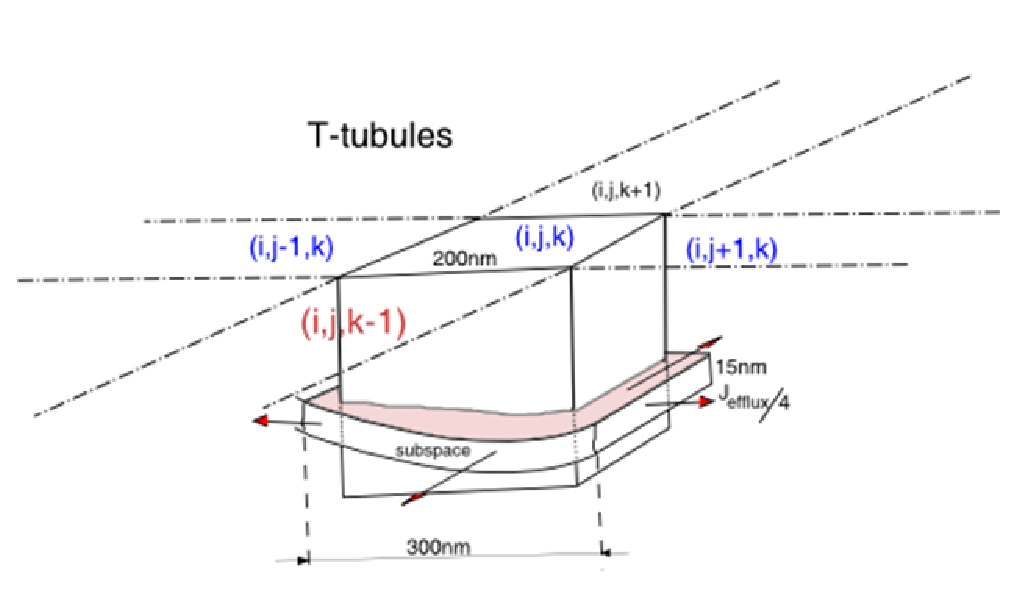
\includegraphics[height=5cm,
    angle=0]{./images/CRU_spatial.eps}}
  \caption{Model of a CRU}
  \label{fig:CRU_spatial}
\end{figure}
 

\chapter{Spatial model with peripheral RyR clusters}
\label{chap:small_RyR_cluster}
% \section{Small RyR cluter}
% \label{sec:small_RyR_cluster}

In cardiac cells, it was observed a small population of ``rogue'' RyR cluster or
non-junctional RyR cluster. The size of these clusters are smaller compared to
those in the dyadic subspace. These rogue RyR clusters are believed to
facilitate the propagation of spark-induced spark. So, it's important to
investigate its role in a spatial-temporal model. This cluster has no apposed
LCC cluter. Currently, the dynamics of these RyR2 channels are assumed the same
as that in the dyadic subspace (\textcolor{red}{so we use the same
rate-transition matrices}). However, some experimental data shown that the
activities of these channels are more often. Thus, we may need to use a
different kinetic scheme for channels in the non-junctional cluster (to be
investigated later).
% \begin{verbatim} !! transition matrices for small RyR clusters (no opposing
% DHPR) REAL(KIND=dp), DIMENSION(:,:), ALLOCATABLE:: aKm2_small, aKp2_small
% INTEGER, DIMENSION(:), ALLOCATABLE :: U_Ro_small INTEGER :: irow_R_small
% \end{verbatim}

\section{New data}

OBSOLETE:
\begin{verbatim}
REAL(KIND=dp), DIMENSION(:,:), ALLOCATABLE:: compK_Rm_small, compK_Rp_small
INTEGER, DIMENSION(:,:), ALLOCATABLE :: idx_Rm_small, idx_Rp_small
INTEGER, DIMENSION(:), ALLOCATABLE :: U_Ro_small
INTEGER :: irow_R_small
INTEGER :: maxnkRm_small, maxnkRp_small  
\end{verbatim}
REPLACED BY
\begin{verbatim}
  !+rogue RyR
  REAL(KIND=dp), DIMENSION(:,:), ALLOCATABLE :: ryr_compKfree_rogue, ryr_compKcal_act_rogue
  INTEGER, DIMENSION(:,:), ALLOCATABLE :: ryr_indxKfree_rogue, ryr_indxKcal_act_rogue
  INTEGER:: ryr_Ncol_Kfree_rogue, ryr_Ncol_Kcal_act_rogue

  !+ vector tells number of open LCC/RyR in each homogeneous cluster space
  REAL(KIND=dp), DIMENSION(:), ALLOCATABLE :: U_Ro_rogue
  !+ number of rows in each vector above
  INTEGER :: irow_R_rogue
\end{verbatim}

For GPU data, we declare

OBSOLETE
\begin{verbatim}
!!for small cluster:
REAL(KIND=dp), DIMENSION(:,:), ALLOCATABLE, device :: compK_Rm_small_dev, compK_Rp_small_dev
INTEGER, DIMENSION(:, :), ALLOCATABLE, device :: idx_Rm_small_dev, idx_Rp_small_dev
REAL(KIND=dp), DIMENSION(:), ALLOCATABLE, device :: U_Ro_small_dev

ALLOCATE(compK_Rm_small_dev(0:maxnkRm_small, irow_R_small), &
       compK_Rp_small_dev(0:maxnkRp_small, irow_R_small), STAT=iserror)
ALLOCATE(idx_Rm_small_dev(0:maxnkRm_small, irow_R_small), &
         idx_Rp_small_dev(0:maxnkRp_small, irow_R_small) )
         
 ALLOCATE(U_Ro_small_dev(irow_R_small), stat=iserror)         
\end{verbatim}
REPLACED BY
\begin{verbatim}
  !!for rogue cluster:
  REAL(KIND=dp), DIMENSION(:,:), ALLOCATABLE, device :: ryr_compKfree_rogue_dev, ryr_compKcal_act_rogue_dev
  INTEGER, DIMENSION(:, :), ALLOCATABLE, device :: ryr_indxKfree_rogue_dev, ryr_indxKcal_act_rogue_dev
  REAL(KIND=dp), DIMENSION(:), ALLOCATABLE, device :: U_Ro_rogue_dev
\end{verbatim}


To generate these matrices, in the main.f95 file, we call
% \begin{verbatim}
%   !! generate transition matrices for small size RyR (no apposing DHPR)
%   CALL makeKs_RyRsmall_2(N_R_small, aKm2_small, aKp2_small, U_Ro_small, irow_R_small)
% \end{verbatim}
\begin{verbatim}
CALL makecompKs_RYRsmall_T(N_R_small, compK_Rm_small, compK_Rp_small,& 
           idx_Rm_small, idx_Rp_small, &
           U_Ro_small, irow_R_small, maxnkRm_small, maxnkRp_small, &
           setupRyR_2state_T) !!! or
CALL makecompKs_RYRsmall(N_R_small, compK_Rm_small, compK_Rp_small, &
           idx_Rm_small, idx_Rp_small, &
           U_Ro_small, irow_R_small, maxnkRm_small, maxnkRp_small, & 
           setupRyR_2state)
\end{verbatim}
and then assign
\begin{verbatim}
    compK_Rm_small_dev = compK_Rm_small
    compK_Rp_small_dev = compK_Rp_small
    idx_Rm_small_dev = idx_Rm_small
    idx_Rp_small_dev = idx_Rp_small
    U_Ro_small_dev = U_Ro_small
\end{verbatim}


%NOTE: We don't need to use compact form as RyR we are using has only 2-state. 

With small size RyR clusters, what need to be changed? 
\section{Size of data array to be increased}
\label{sec:size_data_change}

NOTE: The zero-th entry is important in device kernel for efficient calculation.
In host code, we don't need to use this.

\subsection{Ver 1}
\label{sev:ver_1}

If we assume the peripheral RyR clusters also see a subspace volume, and a
junctional SR, then we need
\begin{enumerate}
  \item number of release sites: though 1\ldots NSFU (regular),
  NSFU+1\ldots (k+1)*NSFU (small size RyR cluster) with k =
  \verb!num_smallRyRneighbors! (1, 3 or 6).
\begin{verbatim}
    ALLOCATE(Ca_ds((num_smallRyRneighbors+1)*NSFU), &
         Ca_jsr((num_smallRyRneighbors+1)*NSFU), PINNED=plog)    

ALLOCATE(Ca_ds_dev(0:(num_smallRyRneighbors+1)*NSFU), &
         Ca_jsr_dev(0:(num_smallRyRneighbors+1)*NSFU), stat=iserror)
\end{verbatim}
With new ``small RyR clusters'', we need to have more fluxes.
\begin{verbatim}
    ALLOCATE(J_efflux_dev(0:(num_smallRyRneighbors+1)*NSFU), &
         J_refill_dev(0:(num_smallRyRneighbors+1)*NSFU), &
         J_ryr_dev(0:(num_smallRyRneighbors+1)*NSFU), stat=iserror)
    
    !!NOTE: I_dhpr_dev not occur in small size RyR cluster
    ALLOCATE(I_dhpr_dev(0:NSFU), stat=iserror)
\end{verbatim}

  \item variable to keep the indices of current states of different CRU
  and rogue RyR clusters is increased in size
  \begin{verbatim}
ALLOCATE(sfu_state((num_smallRyRneighbors+1)*NSFU))
ALLOCATE(RYRgate((num_smallRyRneighbors+1)*NSFU),  DHPRgate(NSFU))

ALLOCATE(RYRgate_dev(0:(num_smallRyRneighbors+1)*NSFU),  &
        stat=iserror)
    
ALLOCATE(sfu_state_dev((num_smallRyRneighbors+1)*NSFU), STAT = iserror)
  \end{verbatim}
  
As we need to manage the states of rogue RyR clusters as well, we need to
modify the subroutine \verb!init_SFU_state!, i.e. replaced by
\verb!init_SFU_state_2!. 

\begin{framed}
SFU is replaced by CRU, i.e. \verb!init_CRU_state_2!. 
\end{framed}
%\verb!init_SFU_state_with_smallRyR!. 

%   \begin{verbatim}
%   ! called from loaddata_from_config()
% CALL init_SFU_state_with_smallRyR(N_L, mL, NUM_STATES_SFU, U_Ro, irow_R,  &
%          irow_R_small, U_Ro_small, sfu_state)
%   \end{verbatim}
  \begin{verbatim}
CALL init_SFU_state_2(N_L, mL, NUM_STATES_SFU, U_Ro, irow_R,  &
         irow_R_small, U_Ro_small, NSFU, sfu_state)
  \end{verbatim}

and
\begin{verbatim}
RYRgate_dev(1:NSFU) = U_Ro(sfu_state(1:NSFU))
RYRgate_dev(NSFU+1:) = U_Ro_small(sfu_state(NSFU+1:))
\end{verbatim}
\end{enumerate}

\subsection{Ver 2}
\label{sec:ver_2}

If we assume the peripheral RyR clusters see the bulk myoplasm and network SR,
then we need
\begin{enumerate}
  \item With new ``small RyR clusters'', we need to have more fluxes.
\begin{verbatim}
    ALLOCATE(J_ryr_dev(0:(num_smallRyRneighbors+1)*NSFU), stat=iserror)
    
    !!NOTE: I_dhpr_dev not occur in small size RyR cluster
    ALLOCATE(I_dhpr_dev(0:NSFU), stat=iserror)
\end{verbatim}

  \item variable to keep the indices of current states of different CRU
  and rogue RyR clusters is increased in size
  \begin{verbatim}
ALLOCATE(sfu_state((num_smallRyRneighbors+1)*NSFU))
ALLOCATE(RYRgate((num_smallRyRneighbors+1)*NSFU),  DHPRgate(NSFU))

ALLOCATE(RYRgate_dev(0:(num_smallRyRneighbors+1)*NSFU),  &
        stat=iserror)
    
ALLOCATE(sfu_state_dev((num_smallRyRneighbors+1)*NSFU), STAT = iserror)
  \end{verbatim}
  
As we need to manage the states of rogue RyR clusters as well, we need to
modify the subroutine \verb!init_SFU_state!, i.e. replaced by
\verb!init_SFU_state_with_smallRyR!. 

  \begin{verbatim}
  ! called from loaddata_from_config()
CALL init_SFU_state_with_smallRyR(N_L, mL, NUM_STATES_SFU, U_Ro, irow_R,  &
         irow_R_small, U_Ro_small, sfu_state)
  \end{verbatim}
and
\begin{verbatim}
RYRgate_dev(1:NSFU) = U_Ro(sfu_state(1:NSFU))
RYRgate_dev(NSFU+1:) = U_Ro_small(sfu_state(NSFU+1:))
\end{verbatim}
\end{enumerate}

\section{Data don't change}

\begin{enumerate}
  \item As we only use the normal release site to determine the time step, we
  don't change \verb!compPdt_dev! size
\begin{verbatim}
	! new method is used by default
    ALLOCATE(compPdt_dev(NSFU,1), stat=iserror)  
\end{verbatim}  

\item The vetor that tell how many DHPR channel opens at each CRU
\begin{verbatim}
ALLOCATE(DHPRgate(NSFU))

DHPRgate_dev = U_Lo(sfu_state(1:NSFU))

\end{verbatim}

\end{enumerate}

\section{Time step}

The adaptive time step is chosen from the normal CRUs, not from the rogue RyR.
So, we only need
\begin{verbatim}
ALLOCATE(compPdt_dev(NSFU,1), stat=iserror)  
\end{verbatim}
rather than
\begin{verbatim}
ALLOCATE(compPdt_dev((num_smallRyRneighbors+1)*NSFU,1), stat=iserror)  
\end{verbatim}

Also, as using the smaller grid point (0.1$\mum^3$,rather than 0.2$\mum^3$), we
need to reduce the time step upper bound from 1d-6 to 2d-7. 

\section{Random numbers}

However, as we simualte stochastically both regular and small size RyR
clusters, we need to change the amount of PRNs to be generated
\begin{verbatim}    
    !X_r_dev = keep pseudo-random numbers
    ALLOCATE(X_r_dev((num_smallRyRneighbors+1)*NSFU*copy_interval)) 
\end{verbatim}
This requires us to use a different function: \verb!init_PRNG_2()!, rather than
\verb!init_PRNG()!, with
\begin{verbatim}
    saruObj = init_saru(NSFU*(num_smallRyRneighbors+1), global_seed)
!!and
    ALLOCATE(X_r((num_smallRyRneighbors+1)*NSFU*copy_interval))
\end{verbatim}

\begin{framed}
NOTE: New code from branch 2 version, use only one function \verb!init_PRNG()!
that work for both regular w/wo rogue cluster of RyRs. 
\end{framed}

\section{Putting rogue RyRs}

UPDATE:
\begin{enumerate}
  \item \verb!_ADD_SMALL_RYRS_! macro is obsolete
  \item Rogue RyRs is replaced for small RyR cluster
  \item Functions to put rougue cluster is explicitly defined in different
  names, allowing us to implement a function to distribute rogue in any place
  easily
  \begin{verbatim}
  put_extra_1_RYRs_cluster
  put_extra_2_RYRs_cluster
  put_extra_3_RYRs_cluster
  put_extra_6_RYRs_cluster
  \end{verbatim}
\end{enumerate}

With rogue RyR, how to know the location of them in the grid? There are
two ways
\begin{enumerate}
  \item if the distance from each rogue RyR cluster to the master CRU is the
  same, we can consider each rogue RyR cluster is a ``pseudo'' CRU, so we
  increase the array to manage location of CRUs in the grid from 1..NSFU to 
  1..(num\_neighborsRyR+1)*NSFU.
  \begin{verbatim}
  allocate(SFU_in_lingrid( (num_smallRyRneighbors+1)*NSFU))
  \end{verbatim}
  Then, we manage them using the information of the CRU and the
  \verb!stride2smallRyR! plus the \verb!num_smallRyRneighbors! (initiated
  inside \verb!init_Simulation()!). For example: the $i$-th CRU has its
  upper neighbor at index (i+NSFU)-th index, left neighbor at (i+2*NSFU)-th
  index\ldots
\begin{verbatim}
!!put_SFU2grid3D_homo_small_RYR()
IF (dist2smallRyR .GT. 0.0d0) THEN 
   !put extra CRU here
            #if _ADD_SMALL_RYRS_ == _1_SMALL_RYRS
   CALL put_extra_1_RYRs_cluster(idx, ii, jj, kk)
            #elif _ADD_SMALL_RYRS_ == _3_SMALL_RYRS
   CALL put_extra_3_RYRs_cluster(idx, ii, jj, kk)
            #elif _ADD_SMALL_RYRS_ == _6_SMALL_RYRS
   CALL put_extra_6_RYRs_cluster(idx, ii, jj, kk)
            #endif

\end{verbatim}  
example:
\begin{verbatim}
!+ one on up
SFU_in_grid3D(idx+NSFU, 1:3) = (/ ii-stride2smallRyR, jj, kk /)
grid3D_with_SFU(ii-stride2smallRyR, jj, kk) = idx+NSFU

lingrid_with_SFU = RESHAPE(grid3D_with_SFU, (/ SIZEWITHBOUNDARY /) )
\end{verbatim}
and modify
\begin{verbatim}
tscell_layout_CaRUs2grid_linear()
\end{verbatim}
to use \verb!put_SFU2grid3D_homo_small_RYR!.

  \item if the distance can be different (using some radomly distribution), we
  need to split the handling of rogue RyR in two separate vectors/matrices:
  \verb!rogueRYR_in_lingrid! and \verb!lingrid_with_rogueRyR!. 
\begin{verbatim}
!data_tscell.f95
INTEGER, DIMENSION(:), ALLOCATABLE :: rogueRyR_in_lingrid
INTEGER, DIMENSION(:), ALLOCATABLE :: lingrid_with_rogueRyR
  !or
INTEGER, DIMENSION(:,:,:), ALLOCATABLE :: grid3D_with_rogueRyR  
\end{verbatim}
by modifying \verb!tscell_allocate_linear()! and
\verb!tscell_allocate_gpu_linear! (to allocate). Here, the size of
\verb!SFU_in_lingrid! doesn't change.

To deal with these two new arrays, we use
\begin{verbatim}
tscell_layout_CaRUsRogueRyR2grid_linear(SFU_in_lingrid, lingrid_with_SFU,
        rogueRyR_in_lingrid, lingrid_with_rogueRyR, put_SFUrogueRyR2grid3D_homo)
\end{verbatim}

\end{enumerate}

\section{Modified kernels}
\label{sec:kernel_change_peripheralRyR}

To set-up kernel configuration, we use \verb!setup_KernelConfiguration_2()!,
rather than \verb!setup_KernelConfiguration()!.
\begin{verbatim}
    CALL setup_KernelConfiguration_2()
\end{verbatim}

\begin{framed}
From branch 2 version, the code use only one name
\verb!setup_KernelConfiguration()! that works for all cases. 
\end{framed}

For kernel to update CRU state, we need to write a new kernel to update
the rogue RyR clusters. There are two options: use the single kernel to update
both CRU and rogue RyRs clusters. However, the code can be divergent. So, we can write two separate
kernels, one to update CRU and one to update rogue RyRs both run in parallel. 
\begin{itemize}
  \item Option 1: Use a single kernel to update both. This kernel uses
\begin{verbatim}
gridSize_smallRyR = CEILING(REAL((num_smallRyRneighbors+1)*NSFU)/blocksize)  
\end{verbatim}
and the kernel to update CRU/rogue-RyR states is
\verb!update_SFU_lin_with_smallRyR!.

\item Option 2: Update CRU and rogue RyRs in two separate kernels. The first one
to update CRUs use
\begin{verbatim}
gridSize = CEILING(REAL(NSFU)/blocksize)
\end{verbatim}
and the second one uses
\begin{verbatim}
gridSize_smallRyR = CEILING(REAL(num_smallRyRneighbors*NSFU)/blocksize)
\end{verbatim}
with the kernel to update CRU is \verb!update_SFU_lin!, and kernel to update
rogue-RyR is \verb!update_rogueRyR!. 
\end{itemize}

To select which approach, they can be reconfigured using macro
\begin{verbatim}
#define _UPDATE_SEPARATE 0
#define _UPDATE_BOTH     1
#define _APPROACH_2_UPDATE_CRU_ROGUERYR _UPDATE_SEPARATE
\end{verbatim}

\subsection{Update states (CRUs + rogue RyRs)}

\subsubsection{First approach}

We use a single kernel to update states of CRUs + rogue RyR clusters
\begin{verbatim}
!! update CRU + rogue RyR clusters in the same kernel
CALL update_SFU_lin_with_smallRyR <<< gridSize_smallRyR, blocksize>>> &
     (X_r_dev((iinner-1)*(num_smallRyRneighbors+1)*NSFU+1:(iinner)*(num_smallRyRneighbors+1)*NSFU), &
     dt, invdt, Vm, kva, kvi, dp_arg1, dp_arg2, &
     Ca_myo_1_dev(PADDING_D+1:), Ca_nsr_1_dev(PADDING_D+1:), &
     time, num_smallRyRneighbors, stride2smallRyR, &
     maxnkRp_small, maxnkRm_small &
     )
\end{verbatim}

\subsubsection{Second approach}

We use two separate kernels: one to update states of CRUs, and one to update
states of rogue RyR clusters.

\begin{verbatim}
CALL update_SFU_lin <<<gridSize, blocksize>>> &
     (X_r_dev((iinner-1)*(num_smallRyRneighbors+1)*NSFU+1:(iinner-1)*(num_smallRyRneighbors+1)*NSFU+NSFU), &
     dt, invdt, Vm, kva, kvi, dp_arg1, dp_arg2, &
     Ca_myo_1_dev(PADDING_D+1:), Ca_nsr_1_dev(PADDING_D+1:), &
     time &
     )
CALL update_rogueRyR <<< gridSize_smallRyR, blocksize>>> &
     (X_r_dev((iinner-1)*(num_smallRyRneighbors+1)*NSFU+NSFU+1:(iinner)*(num_smallRyRneighbors+1)*NSFU), &
     dt, invdt, Vm, kva, kvi, dp_arg1, dp_arg2, &
     Ca_myo_1_dev(PADDING_D+1:), Ca_nsr_1_dev(PADDING_D+1:), &
     time, num_smallRyRneighbors, stride2smallRyR, &
     maxnkRp_small, maxnkRm_small &
     )
\end{verbatim}

\subsection{update\_rogueRYR\_nochangestate}


\verb!update_rogueRYR_nochangestate! accepts \verb!num_rogueRYRneighbors!. It
assumes all CRUs have the same number of rogue-neighbors. 

The assumption above is relaxed in \verb!update_rogueRYR_nochangestate_3!.

\subsection{update\_rogueRYR\_nochangestate\_3}

This version, \verb!update_rogueRYR_nochangestate_3!, accepts
\verb!num_rogueRYRcluster! which is the number of total rogueRYRclusters.

\verb!update_rogueRYR_nochangestate! is the special case of this version where
\begin{verbatim}
num_rogueRYRcluster = num_rogueRYRneighbors * NSFU
\end{verbatim}

\subsection{update\_rogueRYR\_nochangestate\_4}

This version, \verb!update_rogueRYR_nochangestate_4! is an improvement to
\verb!update_rogueRYR_nochangestate_3!, as it allows rogue-RYRcluster to spread
more than one grid-point. User have to update the code and modify the macro
\verb!_ROGUE_LAYOUT_STRATEGY_!.
 
\begin{verbatim}
   #if _ROGUE_LAYOUT_STRATEGY_ == _2x2x1
       INCLUDE "2x2x1_Cansr.inc"
       INCLUDE "2x2x1_Camyo.inc"
   #else
       s_Ca_myo(tx) = Ca_myo(offset)
       s_Ca_nsr(tx) = Ca_nsr(offset)
   #endif    
\end{verbatim}


\subsection{Update grid elements}

We use \verb!update_GridElement_with_rogueRyR!. 


\begin{framed}
IDEA: \textcolor{red}{We may need to convert from using device array to
registers for some variables to increase performance}, e.g. \verb!J_efflux_dev(:)! array
to \verb!J_efflux! variable, \verb!J_refill_dev()!. CHALLENGE: We need to use
them in \verb!ReactTerm_Cmyo! and \verb!ReactTerm_Cnsr!.
\end{framed}

For data in simulation with rogue RyRs, it's better to use the zero-th
index. So, the new formula is

Then, we need special settings
%     Ca_ds_dev(1:NSFU) = Ca_ds(1:NSFU)
%     Ca_jsr_dev(1:NSFU) = Ca_jsr(1:NSFU)
%     Ca_ds_dev(NSFU+1:) = Ca_myo
%     Ca_jsr_dev(NSFU+1:) = Ca_nsr
% 
\begin{verbatim}
    Ca_ds_dev(1:) = Ca_ds
    Ca_jsr_dev(1:) = Ca_jsr

    Ca_ds_dev(0) = 0.0d0
    Ca_jsr_dev(0) = 0.0d0
    J_efflux_dev(0) = 0.0d0
    J_refill_dev(0) = 0.0d0
    J_ryr_dev(0) = 0.0d0
    I_dhpr_dev(0) = 0.0d0
    RYRgate_dev(0) = 0.0d0
    DHPRgate_dev(0) = 0.0d0

    sfu_state_dev = sfu_state
    RYRgate_dev(1:NSFU) = U_Ro(sfu_state(1:NSFU))
    RYRgate_dev(NSFU+1:) = U_Ro_small(sfu_state(NSFU+1:))
    DHPRgate_dev = U_Lo(sfu_state(1:NSFU))
    U_Ro_dev = U_Ro
    U_Lo_dev = U_Lo
    U_Ro_small_dev = U_Ro_small

\end{verbatim}


% The compact-form rate-transition matrices for the small cluster is created by
% this code
% \begin{verbatim}
%     IF (has_smallRyR .EQ. 1) THEN
% #if _USE_TRANSPOSE_FORM_ == _YES
%        CALL makecompKs_RYRsmall_T(N_R_small, compK_Rm_small, compK_Rp_small, &
%             idx_Rm_small, idx_Rp_small, &
%             U_Ro_small, irow_R_small, maxnkRm_small, maxnkRp_small, setupRyR_2state_T)
%        
% #else
%        CALL makecompKs_RYRsmall(N_R_small, compK_Rm_small, compK_Rp_small, &
%             idx_Rm_small, idx_Rp_small, &
%             U_Ro_small, irow_R_small, maxnkRm_small, maxnkRp_small, setupRyR_2state)
%        
% #endif
%     ENDIF
% \end{verbatim}

\section{Code to analyze result}

\subsection{write\_peripheralRyR2file}

The function \verb!write_peripheralRyR2file! prints out data related to trigger
of rogue RyR. It uses
\begin{verbatim}
LOGICAL : is_written2peripheralRyR = .FALSE.
\end{verbatim}
A new variable is needed: \verb!flag5!
\begin{verbatim}
   ! flag5 (tell if CRU/rogueRyR is triggered)  
    ALLOCATE(flag1((num_smallRyRneighbors+1)*NSFU), flag2((num_smallRyRneighbors+1)*NSFU), &
         flag3((num_smallRyRneighbors+1)*NSFU), flag4((num_smallRyRneighbors+1)*NSFU), stat=iserror)
    IF (iserror) PRINT *, "MEM ERROR: flag1, flag2, flag3, flag4"
    ALLOCATE(flag5((num_smallRyRneighbors+1)*NSFU), stat=iserror)
    IF (iserror) PRINT *, "MEM ERROR: flag5"    
    flag1 = .FALSE.
    flag2 = .FALSE.
    flag3 = .FALSE.
    flag4 = .FALSE.
    flag5 = .FALSE.
    ALLOCATE(ts_spark((num_smallRyRneighbors+1)*NSFU), &
         ts_blink((num_smallRyRneighbors+1)*NSFU), stat=iserror)
    IF (iserror) PRINT *, "MEM ERROR: ts_spark, ts_blink"
    ts_spark = +0d0
    ts_blink = +0d0   
\end{verbatim}

The 5 new files are created. Each file print out the corresponding data at the
time all RYRs are opened at normal CRU (first), and then rogue RYRs
\begin{verbatim}
open_time.txt  //time 
open_cmyo.txt  //[Ca2+] at that location
open_CaF.txt   //[CaF] at that location
open_NoRYR.txt // #openRYR at that location
open_Cads.txt  // [Ca]ds at that location 
              // (in the case of atrial cell, it would be the same as
              // open_cmyo.txt)
\end{verbatim}  



\subsection{trigger\_rogue\_RYR}

\verb!trigger_rogue_RYR!, this version does some analysis by triggering the
rogue RyR clusters, not the main CRU.
\begin{verbatim}
  SUBROUTINE trigger_rogue_RYR(U_Ro_small, sfu_state, NSFU, num_smallRyRneighbors, is_all_rogueRyR_open)
\end{verbatim}
This need to uses some variables
\begin{verbatim}
INTEGER, DIMENSION(:), ALLOCATABLE ::  index_rogueRyR_numRyRopen  ! index where #openRyR is 1, 2, ... N_R_small
\end{verbatim}

NOTE: \verb!num_smallRyRneighbor! is replaced by \verb!num_rogueRYRcluster!.


\subsection{trigger\_rogue\_RYR\_3}

\verb!trigger_rogue_RYR_3!, this version relaxes the assumption that all CRUs
have the same number of rogue-RyR cluster. It accepts the total number of
rogue-RYR cluster \verb!num_rogueRYRcluster!.

In this version, all rogueRYRclusters are triggered.

\subsection{trigger\_rogue\_RYR\_4}

\verb!trigger_rogue_RYR_4! is the variant of \verb!trigger_rogue_RYR_3!, as it
allows user to trigger one particular cluster of rogueRYRclusters only. Here, it
assumes there are 3 rogueRYRclusters, and it triggers the second one. 

\section{File changes}
\label{sec:rogueRyR_filechanges}

\subsection{data\_tscell.f95}
\label{sec:data_tscell}

OBSOLETE: \verb!..._small...! becomes \verb!\..._rogue...!

\begin{verbatim}
  INTEGER :: stride2rogueRyR
  REAL(KIND=dp) :: dist2smallRyR
  INTEGER :: num_rogueRyRneighbors = 0, N_R_rogue
  REAL(KIND=dp) :: V_ds_rogue, lambda_ds_rogue, inv_lambda_ds_rogue
  REAL(KIND=dp) :: Ej_rogue
  !REAL(KIND=dp), DIMENSION(:,:), ALLOCATABLE :: ryr_KCal_act_rogue, ryr_Kfree_rogue
\end{verbatim}

New variables:
\begin{verbatim}
  INTEGER :: stride2smallRyR
  REAL(KIND=dp) :: dist2smallRyR
  INTEGER :: num_smallRyRneighbors = 0
  REAL(KIND=dp) :: V_ds_small, lambda_ds_small, inv_lambda_ds_small
\end{verbatim}
then
\begin{verbatim}
    !! prepare ...	
    IF (dist2smallRyR .GT. 0.0d0) THEN 
       !put extra CRU here
#if _ADD_SMALL_RYRS_ == _1_SMALL_RYRS
       ALLOCATE(SFU_in_grid3D(2*NSFU, 3))
       num_smallRyRneighbors = 1
#elif _ADD_SMALL_RYRS_ == _3_SMALL_RYRS
       ALLOCATE(SFU_in_grid3D(4*NSFU, 3))
       num_smallRyRneighbors = 3
#elif _ADD_SMALL_RYRS_ == _6_SMALL_RYRS
       ALLOCATE(SFU_in_grid3D(7*NSFU, 3))
       num_smallRyRneighbors = 6
#else
       WRITE(log_string, *) "Unsupported num neighboring small RyR cluster"
       call write2log(log_string)
       WRITE(log_string, *) "...please, update _ADD_SMALL_RYRS_"
       CALL write2log(log_string)
       STOP       
#endif
       CALL(log_string, *) "num_smallRyRneighbors = ", num_smallRyRneighbors
       CALL write2log(log_string)
    ELSE
#if _ADD_SMALL_RYRS_ != _0_SMALL_RYRS
       WRITE(log_string, *) "Wrong setting with small RyRs"
       CALL write2log(log_string)
       STOP
#endif
       ALLOCATE(SFU_in_grid3D(NSFU, 3))
    END IF
\end{verbatim}
then, a new subroutine is defined to put both normal CRU and rogure RyR clusters
in the mesh grid.
\begin{verbatim}
FUNCTION
  put_SFU2grid3D_homo_small_RYR (SFU_ingrid3D, grid3Dwith_SFU) RESULT (res)
\end{verbatim}


\subsection{tscell\_gpu\_utility.f95}
\label{sec:tscell_gpu_utility}

New variables: to keep track the rate transition of the small clusters of rogue
RyRs
\begin{verbatim}
  REAL(KIND=dp), DIMENSION(:,:), ALLOCATABLE, device :: compK_Rm_small_dev, compK_Rp_small_dev
  INTEGER, DIMENSION(:, :), ALLOCATABLE, device :: idx_Rm_small_dev, idx_Rp_small_dev
  REAL(KIND=dp), DIMENSION(:), ALLOCATABLE, device :: U_Ro_small_dev
\end{verbatim}
with data allocation
\begin{verbatim}
    ALLOCATE(compK_Rm_small_dev(0:maxnkRm_small, irow_R_small), &
         compK_Rp_small_dev(0:maxnkRp_small, irow_R_small), STAT=iserror)
    IF (iserror .NE. 0) PRINT *, "MEM ERROR: compK_Rm_small_dev..."
    ALLOCATE(idx_Rm_small_dev(0:maxnkRm_small, irow_R_small), &
         idx_Rp_small_dev(0:maxnkRp_small, irow_R_small) )
    IF (iserror .NE. 0) PRINT *, "MEM ERROR: index_Rm_small_dev, ..."
    
    ALLOCATE(U_Ro_small_dev(irow_R_small), stat=iserror)
    IF (iserror) PRINT *, "MEM ERROR: U_Ro_small_dev" 
\end{verbatim}
The gating for these small clusters are contained in the extended vector of
\verb!RYRgate_dev()! (NOTE: there is no change in \verb!DHPRgate_dev()!)
\begin{verbatim}
    ALLOCATE(RYRgate_dev(0:(num_smallRyRneighbors+1)*NSFU),  &
         DHPRgate_dev(0:NSFU), stat=iserror)
\end{verbatim}

The vector \verb!sfu_state_dev()! that keeps the current state index is
also extended. 
\begin{verbatim}
    ALLOCATE(sfu_state_dev((num_smallRyRneighbors+1)*NSFU), STAT = iserror)
\end{verbatim}
NOTE: from 1..NSFU, it keeps index for vector \verb!U_Ro!, while from
NSFU+1\ldots to the end, it keeps the index for vector \verb!U_Ro_small!. 

As the gating for channels in these small clusters are stochastic as well, we
also extend the number of generated pseudo-random numbers
\begin{verbatim}
!X_r_dev = keep pseudo-random numbers
    ALLOCATE(X_r_dev((num_smallRyRneighbors+1)*NSFU*copy_interval), stat=iserror) 
    IF (iserror) PRINT *, "MEM ERROR: X_r_dev"
\end{verbatim}
NOTE: We need to modify \verb!init_PRNG()! to \verb!init_PRNG_2()!.

% Also, we assume there is a small subspace area in these small cluster, so with
% $N$ such small clusters, we need to have $N$ new calcium subspace. To make it
% easier to handle, we extend the array \verb!Ca_ds_dev()! and \verb!Ca_jsr_dev()! to
% \begin{verbatim}
%     ALLOCATE(Ca_ds_dev(0:(num_smallRyRneighbors+1)*NSFU), &
%          Ca_jsr_dev(0:(num_smallRyRneighbors+1)*NSFU), stat=iserror)
%          
%     ALLOCATE(Ca_ds_prev_dev(0:(num_smallRyRneighbors+1)*NSFU), stat=iserror) 
% \end{verbatim}
% along with these subspaces, we also need addition fluxes variables, so we also
% extend the vectors of the fluxes
% \begin{verbatim}
%     ALLOCATE(J_efflux_dev(0:(num_smallRyRneighbors+1)*NSFU), &
%          J_refill_dev(0:(num_smallRyRneighbors+1)*NSFU), &
%          J_ryr_dev(0:(num_smallRyRneighbors+1)*NSFU), stat=iserror)
%     J_efflux_dev = +0d0; J_refill_dev = +0d0; J_ryr_dev = +0d0
% \end{verbatim}
% NOTE: The zero-th entry is important in device kernel for efficient calculation.
% In host code, we don't need to use this


% In kernel, we have some changes: we have another grid size to work with both
% normal and small clusters
% \begin{verbatim}
% blocksize = BLOCKSIZE_1D
% gridSize = CEILING(REAL(NSFU)/blocksize)
% gridSize_smallRyR = CEILING(REAL((num_smallRyRneighbors+1)*NSFU)/blocksize)  ! ceiling value
% \end{verbatim}

For other data changes, see Sect.\ref{sec:size_data_change}. For kernel changes,
see Sect.\ref{sec:kernel_change_peripheralRyR}.
 
\section{Name changes}

\begin{enumerate}
  \item We change \verb!_small! to \verb!_rogue!, e.g
  \begin{verbatim}
  INTEGER :: num_rogueRyRneighbors
  \end{verbatim}
  So, the new names are
  \begin{verbatim}
  lambda_ds_small     -->   lambda_ds_rogue
  inv_lambda_ds_small -->   inv_lambda_ds_rogue
  V_ds_small          -->   V_ds_rogue
  N_R_small           -->   N_R_rogue
  E_j_small           -->   E_j_rogue
  \end{verbatim}
  The transition matrices and indexing matrices as well
  \begin{verbatim}
  compK_Rm_small      -->   ryr_compKfree_rogue
  compK_Rp_small      -->   ryr_compKcal_act_rogue3
  \end{verbatim}
  
\end{enumerate}


\chapter{Spatial Model Atrial Cell}
\label{chap:spatial_atrial_cell}


There are major change in coding the model for atrial cells. This is mainly
caused by the fact that in atrial cell, the microdomain of subspace is very
rarely (10-20\%). So most of the time, the ryanodine receptor (RyR2) see the calcium in the myoplasm. 
To study the dynamics of calcium sparks, in the model, we removed this effect by
making some changes in the temporalspatial code.

\begin{enumerate}
  \item  \verb!Ca_ds_dev! is removed from the code, instead we replace it with
  \verb!Ca_myo_in(offset)! with \verb!offset=SFU_in_lingrid_dev(ii)! with $ii$
  is the index of the 'pseudo'-SFU in which we still use to detect the jSR location. 
 
 \item As a matter of fact, the calcium from $I_\dhpr$ and $J_\ryr$ flow directly into
the grid point containing myoplasm. So, we don't need to have
\verb!J_efflux! nor \verb!J_efflux_part! in the code.

\begin{verbatim}
J_efflux_dev(ii) = J_dhpr + J_ryr_dev(ii)
J_efflux_part_dev(offset) = J_efflux_dev(ii)
\end{verbatim}

 \item Using of \verb!_CRU_LAYOUT_STRATEGY_! macro is removed. Also, the flux
 rate need to be adjusted
\begin{verbatim}
v_ryrT = ???
P_dhprT = ???
\end{verbatim}
NOTE: This is permeabilized cell, so we run \verb!_MODE_CLOSED_CELL! simulation,
and we don't use \verb!P_dhprT! value.

  \item The detection of the peak of the spark is now using
  \verb!Ca_peak_prev_dev! rather than \verb!Ca_ds_prev_dev!. 
  
  \item Some functions has been modified to adapt to atrial cell
  \begin{verbatim}
  analyze_Sparks_2(... , Ca_myo_in)
  analyze_Sparks_3(... , Ca_myo_in)
  \end{verbatim}
  
  \item New macro to determine blocking SERCA or not
  \begin{verbatim}
  #define _USE_SERCA_ _YES
  \end{verbatim}
  
  \item New macro to incorporate the effect of EGTA buffer
  \begin{verbatim}
    #define _USE_EGTA_ _YES
  \end{verbatim}
\end{enumerate}

The code works with grid-point of size 100nm and 50nm. 
\begin{enumerate}
  \item 49RYR: it senses calcium from 300x200x100 (which uses macro
  \verb!_3x2x1! or \verb!_6x4x2!, depending on the grid-size being used)
  \item 25RYR: it senses calcium from 200x200x100 (which uses macro
  \verb!_2x2x1! or \verb!_4x4x2!)
\end{enumerate}

\textcolor{red}{All simulations were done under the condition of permeabilized
cells}, i.e. no change in cytoplasmic calcium. The exogenous buffer EGTA was
incorporated to avoid calcium waves.

The major change in AF compared to Ctrl is the buffer changes, and an increase
in the number of sattelite clusters. In Ctrl, it has about 2 satellite clusters,
at a distance within 150nm that form the super-cluster or a functioning group
with the center cluster. In AF, it has about 4 satellite clusters. Also,
macrosparks are observed more frequently in AF (from very rarely in Ctrl to
about 10\% in AF), a simulation using 50nm grid-size was done. 


\section{Macro-sparks}

We do two things to test macro-sparks

\begin{enumerate}
  \item One big cluster (384RyRs), the activation is 
\begin{verbatim}
//macro.h
#define _ARRANGE_CRU_ _CRU_UNIFORM_WITH_ROGUE_RYR
#define _CRU_LAYOUT_STRATEGY_ _9x9x1
#define _EMULATE_CONDITION_ _CUSTOMIZED_CRUS
\end{verbatim}  
and no rogue RyR setting.

  \item Use a customize CRU arrangement setting  
\begin{verbatim}
//macro.h
#define _ARRANGE_CRU_ _CRU_MACROSPARK_WITH_ROGUE_RYR

//tscell_gpu_utility.f95
  #elif _ARRANGE_CRU_ == _CRU_MACROSPARK_WITH_ROGUE_RYR
    ierr = tscell_layout_CaRUs2grid_linear(NSFU, SFU_in_lingrid, lingrid_with_SFU, &
         put_SFU2grid3D_macrospark_rogue_RYR)

\end{verbatim}
\end{enumerate}


Also, the activation of the cluster is depending on the calcium highest among
the grid-points covered by the RyR cluster, rather than the averaged calcium
level at these grid-points.
\begin{enumerate}
  \item 9x9x1
\begin{verbatim}
!!9x9x1
       s_Ca_myo(tx) = 0.0d0
       do mi = -4, 4
             dtemp = maxval(Ca_myo(offset+mi*int_ca(17)-4 : offset+mi*int_ca(17)+4))
             s_Ca_myo(tx) = max(s_Ca_myo(tx), dtemp)
       end do
\end{verbatim}

  \item 3x3x1
\begin{verbatim}
!!3x3x1
       s_Ca_myo(tx) = 0.0d0
       do mi = -1, 1
             dtemp = maxval(Ca_myo(offset+mi*int_ca(17)-1 : offset+mi*int_ca(17)+1))
             s_Ca_myo(tx) = max(s_Ca_myo(tx), dtemp)
       end do
\end{verbatim}  
\end{enumerate}




\chapter{Updates/Plans}
\label{sec:updates}

\section{Update parameter file}
\label{sec:parameter-file}

change parameter files:
\begin{enumerate}

\item  substitute \verb!v_ryr_nj!
\begin{verbatim}
replace v_ryr_nj --> prcent_ryr (i.e. 5% or 0.05)
\end{verbatim}

\item substitute \verb!P_dhpr_nj!
\begin{verbatim}
replace P_dhpr_nj --> prcent_dhpr-nj (i.e. 10% or 0.1)
\end{verbatim}


\item substitute \verb!P_dhpr_T!
\begin{verbatim}
replace P_dhpr_T --> i_1dhpr
\end{verbatim}
and add scaling macro \verb!_USE_SCALING_MODEL_! to determine whether
scaling is used or not. 

\item add 3 parameters after \verb!t_end! and before \verb!dt_LB! (Jan, 14,
2012)
\begin{verbatim}
0.0d0         first_beat I/O (0=No / 1=Yes)
2.0d0         last_beats I/O (duration) [sec]
0.0d0         use_restart_file (0=No / 1=Yes)
\end{verbatim}
then, data mode \verb!_IO_RESTART_FILE! is removed. 
\end{enumerate}

\subsection{Affect leak model}
\label{sec:affect-leak-model}

\begin{enumerate}
\item change the name for specific membrane capacitance
\begin{verbatim}
Cm --> Csc
\end{verbatim}
as Cm will be used for whole-cell membrane capacitance.

\item change variables for buffering fractions (to discriminate with buffer
  concentration \verb!B_myoT!...)
\begin{verbatim}
B_ds --> beta_ds  
B_nsr --> beta_nsr
B_myo --> beta_myo
B_jsr --> beta_jsr
\end{verbatim}



\item change variable
\begin{verbatim}
! to indicate total ryr_nj transfer rate, not a single channel
v_ryr_nj --> v_ryr_nj_T
\end{verbatim}


\item change variable (to discriminate half-saturation constant Km vs. dissociation
  constant Kd)
\begin{verbatim}
Kd_myo --> Km_myo
Kd_jsr --> Km_jsr
\end{verbatim}

\item change volume ratio variables
\begin{verbatim}
lambda1 --> lambda_ds
lambda2 --> lambda_jsr
lambda  --> lambda_nsr
\end{verbatim}

\item change variable
\begin{verbatim}
Mbig --> NUM_STATES_SFU
\end{verbatim}

\item Automatically renames all parameters to ``parameter.conf'' so that it's
easier to read code in IDL.
\begin{verbatim}
CHARACTER(MAX_FILENAME) :: default_param_filename = 'parameters.conf'
\end{verbatim}

\item The variable \verb!ID_logfile! is replaced by \verb!log_string! and call
to \verb!write2log(log_string)!. 
\end{enumerate}

\subsection{Affect EC-coupling}
\label{sec:ec-coupling-1}

\begin{enumerate}
\item Move vv1, vv2 to \verb!Vm_dependent.inc! file, and add to the
  code via
\begin{verbatim}
INCLUDE "Vm_dependent.inc"
\end{verbatim}


\item Change the variables for random numbers
\begin{verbatim}
X     --> X_r
X_dev --> X_r_dev
\end{verbatim}


\item move \verb!sfu_state! to file: \verb!data_ecc.f95!

\item rename vv1, vv2
\begin{verbatim}
vv1 --> kva
vv2 --> kvi
\end{verbatim}


\item name change
\begin{verbatim}
isfu --> current_state_sfu --> sfu_state
isfu_dev --> current_state_sfu_dev --> sfu_state_dev
\end{verbatim}

\item change maxnk\ldots (with new algorithms)
\begin{verbatim}
maxnkv1 --> lcc_Ncol_Kv_act
maxnkv2 --> lcc_Ncol_Kv_inact
maxnkp1 --> lcc_Ncol_Kcal_inact
maxnkm1 --> lcc_Ncol_Kfree
maxnkm2 --> ryr_Ncol_Kfree
maxnkp2 --> ryr_Ncol_Kcal_act
\end{verbatim}

\item change \verb!sfu_state! 
\begin{verbatim}
sfu_state --> CRU_states
\end{verbatim}

\item change idxK, compK \ldots 
\begin{verbatim}
compKv1 --> lcc_compKv_act
compKv2 --> lcc_compKv_inact
compKp1 --> lcc_compKcal_inact
compKm1 --> lcc_compKfree
compKm2 --> ryr_compKfree
compKp2 --> ryr_compKcal_act
       
idxKv1 -->  lcc_indxKv_act
idxKv2 --> lcc_indxKv_inact
indxKm1 --> lcc_indxKfree
idxKm2 --> ryr_indxKfree
indxKp1 --> lcc_indxKcal_inact
indxKp2 --> ryr_indxKcal_act
\end{verbatim}

\item move \verb!init_GPU()! from \verb!data_global.f95! to
\verb!cuda_interop.f95!

\item move \verb!mL, mR! to the 2 new parameter files

\item rename \verb!is_Clamped! to \verb!is_being_clamped!

\item rename (to match with the similar function in spatial code) [2012-Nov-20]
\begin{verbatim}
updateSystem_2 --> update_SFU_2
updateSystem_2b --> update_SFU_2b
\end{verbatim}
\end{enumerate}

\subsection{Affect Spatial model}
\label{sec:affect-spatial-model}

\begin{enumerate}
\item Remove \verb!inv_RT_F!, the equivalent to use is \verb!F_RT!
\item Diffusion is now allows to be anisotropic at both calcium-bound
fluorescence and fluorescence with \verb!D_F! and \verb!D_CaF! are replaced by 
\begin{verbatim}
 REAL(KIND=dp), constant :: D_Fx, D_Fy, D_Fz, D_CaFx, D_CaFy, D_CaFz
\end{verbatim}

\item SFU is replaced by CRU as SFU refer to a functional group of RyRs only.
CRU refers to a fusion of RyR and LCCs. 
\begin{verbatim}
init_SFU_state --> init_CRU_state
sfu_state --> CRU_state
\end{verbatim}

\item Rename
\begin{verbatim}
some_caffeinedump_CRU_notfullyOpen --> some_caffeineBound_CRU_notfullyopen
num_timesteps_before_setting_allchannels_open --> num_timesteps_holdingchannels
\end{verbatim}

\item Rename 
\begin{verbatim}
_CRU_UNIFORM_WITH_SMALL_RYR --> _CRU_UNIFORM_WITH_ROGUE_RYR
\end{verbatim}

\item Rename [2013-Jan-29]
\begin{verbatim}
put_SFU2grid3D_homo           --> put_SFU2grid3D_uniform
put_SFU2grid3D_homo_rogue_RYR --> put_SFU2grid3D_uniform_rogue_RYR
\end{verbatim}
\end{enumerate}

% \item change parameter files: 
% \begin{verbatim}
% replace v_ryr_T --> i_1ryr (current single ryr channel)
% \end{verbatim}

% \item change $zCa$ to \verb!z_Ca!
% \begin{verbatim}
% zCa -> z_Ca
% zNa -> z_Na
% zK  -> z_K
% \end{verbatim}

% \item change zF to \verb!frdy! (Faraday constant)

% \item change zR to \verb!uniR! (universal gas constant)

%\end{enumerate}

\subsection{Affect Spatial Model with neighboring cluster}

\begin{enumerate}
  \item \verb!stride2smallRyR! is replaced by \verb!stride2rogueRyR!
  \item The macro name \verb!_ADD_SMALL_RYRS_! is replaced by a read-in value in
  the parameter file \verb!testspatialdata_file.txt!
  \begin{verbatim}
 6.0000E+0      num rogue RyR-neighbors (0,1,2,3,6)
 5.0000E+0      num RyRs in rogue cluster
  \end{verbatim}
  
  \item \verb!stride2rogueRyR! is extended and replaced by 6 variables
  \begin{verbatim}
  stride2rogueRyR_x_up, stride2rogueRyR_x_down
  stride2rogueRyR_y_left, stride2rogueRyR_y_right
  stride2rogueRyR_z_front, stride2rogueRyR_z_back
  \end{verbatim}
  The reason is that subspace is not a the same in all dimension but has the
  following dimension 15nm x 200 nm x 350nm. 
  
  \item The following code is removed from branch 2 version
  \begin{verbatim}
INTEGER, DIMENSION(:), ALLOCATABLE ::  index_CRUstate_numRyRopen  ! CRUstate index where #openRyR is 1, 2, ... N_R
INTEGER, DIMENSION(:), ALLOCATABLE ::  index_rogueRyR_numRyRopen  ! index where #openRyR is 1, 2, ... N_R_small
  \end{verbatim}
  
  
  \item \verb!dist2rogueRyR! tell the distance from
  center-CRU to the satellite RYR cluster (old-name: \verb!dist2smallRYR!,
  \verb!dist2satelliteRYRs!) [2014-Apr-18]
\end{enumerate}

\section{Plans}
\label{sec:plans}

\begin{enumerate}
  \item create the reference volume Vol$_{ref}$ which is assigned to $V_\myo^T$
  by default, and then replace 
  \begin{verbatim}
  Am_2FVmyo    ---> Am_2FV
  Am_FVmyo     ---> Am_FV
  inv_2FVmyo   ---> inv_2FV
  \end{verbatim}
\item (parameter file)  remove if not in used
\begin{verbatim}
V_theta2
V_sigma2
\end{verbatim}

\item (parameter file) remove Ej as it can be calculated from \verb!N_R!. 
\begin{verbatim}
Ej =1/(sqrt(N_R)*(sqrt(N_R)-1))((sqrt(N_R)-2)^2*4+(sqrt(N_R)-2)*4*3+4*2)
\end{verbatim}


\item Add junctional NCX  \verb!I_ncx_j! to the ECC non-spatial model
  and probably the spatial model
\begin{verbatim}
## in each CRU
I_ncx_j  = I_ncx_bar_j*(na_i^3*ca_o*EXP(0.35*V/RT_F)-na_o^3*ca_ds*EXP((0.35-1)*V/RT_F))./
         ((87500^3+na_o^3)*(1380+ca_o)*(1+0.1*EXP((0.35-1)*V/RT_F)))
J_ncx_j = -2*I_ncx_j*Am_2FVmyo
# which contribute to [Ca]_ds
\end{verbatim}

\item Remove in spatial model

\begin{verbatim}
J_efflux_total
J_refill_total
I_dhpr_total
\end{verbatim}


\item instead of using \verb!sum_reduce_double_2host()!, define a
  kernel that can be called from Fortran so that 2 kernels can run at
  the same time using 2 different stream IDs.


\item add to the spatial code
\begin{verbatim}
ts_Na_lin
ts_K_lin
\end{verbatim}
to functions
\begin{verbatim}
tscell_initialize_linear
...
\end{verbatim}


\item Consider spatial heterogeneous distribution of NCX where NCX is
  present more in junctional SR, or along the T-tubules. 


\item Implement \verb!makeKs_nj()! that work with any number of states
  for  RyR and DHPR


\item \sout{Remove 2 output set of columns RyRGate() and
  DHPRgate() from HDF files (and rerun all restart files with
  control, HF, and HForphan...)}


\item Consider moving caffeine setting to the \verb!testdata_file.txt!

\item \sout{Add the param file name in the summary\_data.txt so that we
don't have to search for correc tconfiguration file name. (add to the first
line)}

\item Implement print out to restart file \verb!datamode6_init!,
\verb!datamode6_print!, \verb!datamode6_print_last!.

\item Change in spatial code to reflect better name (flux from SR to MYO should
be flux from internal source (either NSR or subspace) to MYO)
\begin{verbatim}
J_sr2myo ---> J_int2myo
\end{verbatim}


\end{enumerate}


\chapter{Data I/O}
\label{chap:Data_IO}

\begin{lstlisting}
CALL data_io_init()

CALL data_io_write()

CALL data_io_finalize()
\end{lstlisting}
which will call appropriate I/O functions depending on the setting of
macro values. 

There are a number of modes
\begin{verbatim}
#define _IO_NONE  0  
#define _IO_TEST  1
#define _IO_2_HDF  2
#define _IO_2_ASCII  3
#define _IO_2_SILO_3D 4 
#define _IO_2_SILO_SLICE 5
#define _IO_RESTART_FILE 6 
#define _IO_2_HDF2 7

#define _DATAMODE_ _IO_RESTART_FILE
\end{verbatim}
The description for each mode is given as follows
\begin{verbatim}
  !   0 = no I/O (only summary file is written)
  !   1 = testing purpose (we can freely modify to print out 
  !        (what we want in ASCII format)
  !   2 = (spatial or non-spatial) HDF files
  !   3 = text files (all)
  !   4,5 = spatial output
  !   6 = write out restart file and the last second
  !   7 = (non-spatial) multiple datasets/file (time-Vm, Cads, Cajsr...)
  !   8 = (spatial) HDF whole-cell
NOTE: restart file is written out in all cases, except _IO_NONE  
\end{verbatim}
All modes print out the restart files. In mode \verb!_IO_RESTART_FILES!, we also
print out the last second.

We have two time trackers:
\begin{verbatim}
time_prev1 = to keep track when to write data out
time_prev2 = to keep track time for calculating integrate flux
time_prev_fb = to keep track when to write data out in first-second
\end{verbatim}


\section{Leak code}
\label{sec:IO_leak}

It still uses 
\begin{verbatim}
#if _DATAMODE_ == 1
    CALL datamode1_print()
#elif _DATAMODE_ == 2
    CALL datamode2_print()
#elif _DATAMODE_ == 3
    CALL datamode3_print()
#endif
\end{verbatim}

\section{ECC code}
\label{sec:IO_ecc}

Even though there are many options to choose the output format (as
described in the below subsections), there are another two options to choose how
often you want to do I/O
\begin{enumerate}
  \item \verb!_METHOD1!: write every \verb!x! (sec) with \verb!x! read from
  parameter file
  \item \verb!_METHOD2!: write after a given number of iterations (default: 100)
\end{enumerate}

\subsection{\_IO\_2\_HDF}
\label{sec:ECC_HDF}

Old versions: data is organized in a single data set ``/LEAK'' with a large
number of columns. The functions for \verb!_IO_2_HDF!, it uses
\begin{verbatim}
datamode2_init()
datamode2_print()
  CALL hdf_open_simple(file_out, NSFU, CHUNK_SIZE, CHUNKS_PER_FILE, 
                   file_struct, FIELDS_PER_RECORD)
  CALL hdf_write_simple(file_struct, data_buffer, CHUNK_SIZE, 
                   FIELDS_PER_RECORD)
  CALL hdf_spark_close(file_struct)

datamode2_print_last()       
datamode2_close()
\end{verbatim}

\subsection{\_IO\_2\_HDF2}
\label{sec:ECC_HDF2}

New version: data is organized into a number of datasets
\begin{enumerate}
  \item ``/general''
  \item ``/sfu-state''
  \item ``/cds''
  \item ``/cjsr''
  \item ``/cacm''
\end{enumerate}
The functions for \verb!_IO_2_HDF2!, it uses
\begin{verbatim} 
datamode7_init()
datamode7_print()
  CALL hdf_ecc_open(file_out, NSFU, CHUNK_SIZE, 
                       CHUNKS_PER_FILE, file_struct, FIELDS_PER_RECORD)
  CALL hdf_ecc_write(file_struct, data_buffer, CHUNK_SIZE, 
                       FIELDS_PER_RECORD, NSFU)
  CALL hdf_ecc_close(file_struct)

datamode7_close()
\end{verbatim}



\section{Spatial code}
\label{sec:IO_spatial}

Here, we want to make sure all files have the same number of time points, so we
decided to divide files into a number of categories:
\begin{enumerate}
  \item \verb!file_struct! (HDFFILE): non-spatial or regular data (Vm, Cads,
  Cajsr, etc.)
  \item \verb!file_struct_cmyo! (HDFFILE2, HDFFILE3)
  \item \verb!file_struct_caf! (HDFFILE2, HDFFILE3)
  \item \verb!file_struct_cnsr! (HDFFILE2, HDFFILE3)
  \item \verb!file_struct_Incx! (HDFFILE2, HDFFILE3)
  \item (future) \ldots 
\end{enumerate}
\begin{verbatim}
  TYPE(HDFFILE) :: file_struct
#if _DATAMODE_ == _IO_2_HDF  
  TYPE(HDFFILE2) :: file_struct_cmyo, file_struct_CaF, file_struct_cnsr
#elif _DATAMODE_ == _IO_2_HDF3D
  TYPE(HDFFILE3) :: file_struct_cmyo, file_struct_CaF, file_struct_cnsr
  TYPE(HDFFILE3) :: file_struct_Incx
#endif
\end{verbatim}
with the description of each type as follows
\begin{verbatim}
  TYPE HDFFILE !regular data
     INTEGER(HID_T) :: file_ID
     INTEGER(HID_T), DIMENSION(MAX_NUM_HANDLE) :: arr_dspace ! (data) space
     INTEGER ::  num_dspace
     INTEGER(HID_T), DIMENSION(MAX_NUM_HANDLE) :: arr_dset ! dataset
     INTEGER :: num_dset
     INTEGER(HID_T), DIMENSION(MAX_NUM_HANDLE) :: arr_plist !property list
     INTEGER :: num_plist
  END TYPE HDFFILE
\end{verbatim}

Each file has one chunk (\verb!CHUNKS_PER_FILE=1!). Each chunk is a table of
size \verb!CHUNK_SIZE! x \verb!FIELDS_PER_RECORD!, with
\begin{verbatim}
    CHUNK_SIZE = 20000
    CHUNKS_PER_FILE = 1 ! set it to one for now
    NUM_STATES_NJ = mR * mL
    NUM_FIELDS4CURRENTS = 11
    !2 columns = 1 for time + 1 for Vm
    !first NSFU = sfu_state
    !second NSFU = cds
    !third NSFU = cjsr
    FIELDS_PER_RECORD = 2 + NSFU + NUM_STATES_NJ + NUM_FIELDS4CURRENTS + 2*NSFU
\end{verbatim}
 
\begin{verbatim}
  TYPE HDFFILE2 !to deal with spatial data
     INTEGER(HID_T) :: file_ID
     INTEGER(HID_T), DIMENSION(MAX_NUM_HANDLE) :: arr_dspace ! (data) space
     INTEGER ::  num_dspace
     !first = vlayer
     !second= hlayer
     INTEGER(HID_T), DIMENSION(2,MAX_NUM_HANDLE,MAX_NUM_GROUPS) :: arr_dset ! dataset (1:2,dataset_id, group_id)
     INTEGER, DIMENSION(MAX_NUM_HANDLE) :: num_dset !number of dset in each group
     INTEGER(HID_T), DIMENSION(MAX_NUM_HANDLE) :: arr_plist !property list
     INTEGER :: num_plist
     INTEGER(HID_T), DIMENSION(MAX_NUM_GROUPS) :: arr_group ! group
     INTEGER :: num_group
     !the zero-th element keep the number of elements in the array
     REAL(KIND=dp), DIMENSION(MAX_NUM_HANDLE*MAX_NUM_GROUPS) :: time_data
  END TYPE HDFFILE2
\end{verbatim}

\begin{verbatim}
  TYPE HDFFILE3 !spatial whole-cell data
     INTEGER(HID_T) :: file_ID
     INTEGER(HID_T), DIMENSION(MAX_NUM_HANDLE) :: arr_dspace ! (data) space
     INTEGER ::  num_dspace
     INTEGER(HID_T), DIMENSION(MAX_NUM_HANDLE) :: arr_dset ! dataset
     INTEGER :: num_dset
     INTEGER(HID_T), DIMENSION(MAX_NUM_HANDLE) :: arr_plist !property list
     INTEGER :: num_plist
     REAL(KIND=dp), DIMENSION(MAX_NUM_HANDLE) :: time_data
  END TYPE HDFFILE3
\end{verbatim}

\subsection{\_IO\_2\_HDF}

We print out 2 layers (longitudinal and transversal direction) at each Z-lines.
The mode is \verb!_IO_2_HDF2!, it uses
\begin{verbatim}
datamode2_init_2()
datamode2_print_2()
    CALL get_new_cmyo_filename(hdf_cmyo_filename, hdf_spatial_fileindex)
    CALL hdf_spatial_open(file_struct_cmyo, hdf_cmyo_filename, num_vlayers, num_hlayers, &
         outerDIMX, outerDIMY, outerDIMZ)
    CALL get_cnsr_filename(hdf_cnsr_filename, hdf_spatial_fileindex)
    CALL hdf_spatial_open(file_struct_cnsr, hdf_cnsr_filename, num_vlayers, num_hlayers, &
         outerDIMX, outerDIMY, outerDIMZ)
  #if _USE_FLUO_ != _NO
    CALL get_CaF_filename(hdf_CaF_filename, hdf_spatial_fileindex)
    CALL hdf_spatial_open(file_struct_CaF, hdf_CaF_filename, num_vlayers, num_hlayers, &
         outerDIMX, outerDIMY, outerDIMZ)
  #endif
    CALL hdf_spatial_write(file_struct_cmyo, ts_Ca_myo, &
         num_vlayers, idx_vlayers, num_hlayers, idx_hlayers, &
         outerDIMX, outerDIMY, outerDIMZ, time, file_is_full)

    CALL hdf_spatial_write(file_struct_cnsr, ts_Ca_nsr, &
         num_vlayers, idx_vlayers, num_hlayers, idx_hlayers, &
         outerDIMX, outerDIMY, outerDIMZ, time, file_is_full)

    CALL hdf_open_simple(file_out, NSFU, CHUNK_SIZE, CHUNKS_PER_FILE, file_struct, FIELDS_PER_RECORD)
    CALL hdf_write_simple(file_struct, data_buffer, CHUNK_SIZE, FIELDS_PER_RECORD)
    CALL hdf_spark_close(file_struct)
  
datamode2_close_2()
\end{verbatim}
Given the number of time points is CHUNK\_SIZE=10,000; we divide the
spatial data in HDF5 into 100 groups, each group has 2x100 datasets (first 100
belongs to cmyo-vertical, second 100 belongs to cmyo-horizontal).

\begin{framed}
Using 10,000 dataset per file, it gives 15GB of data. So, we suggest using
300 dataset per file, which gives 500MB per file.
\end{framed}
Here, we use two different file indices, one for HDF5 spatial data
\verb!hdf_spatial_fileindex!, and one for HDF5 regular data \verb!file_index!. 

The HDF4 spatial code is organized as follows:
\begin{enumerate}
  \item 4 groups. Name of groups /group-001, /group-002\ldots, each group has 2x100
  datasets.
  \item the first 100 dataset 
\end{enumerate}

For cmyo spatial data, we do
\begin{verbatim}
hdf_spatial_fileindex = 0 !deal with spatial data
hdf_groupindex = 0  ! deal with group
hdf_datasetindex_ingroup = 0 ! deal with dataset in the current group
!automatically increase file index and return the file name
CALL get_new_cmyo_filename(hdf_cmyo_filename, hdf_spatial_fileindex)
CALL hdf_spatial_open(file_struct_cmyo, hdf_cmyo_filename, hdf_groupindex, num_vlayers, num_hlayers, &
     outerDIMX, outerDIMY, outerDIMZ)
\end{verbatim}

In \verb!hdf_spatial_open!, it does
\begin{enumerate}
  \item We create the file
\begin{verbatim}
CALL h5fcreate_f(TRIM(filename), H5F_ACC_TRUNC_F, file_ID, hdf_error, &
         H5P_DEFAULT_F, H5P_DEFAULT_F)
file_struct%file_ID = file_ID
\end{verbatim}

%\item We create attribute for root group (/) to store some information

\item We create the group
\begin{verbatim}
    !create the first group
    WRITE(group_name, "('/group-', i3.3)") group_index
    CALL h5gcreate_f(file_ID, TRIM(group_name), hdf_error, 0)
    file_struct%num_group = file_struct%num_group + 1
\end{verbatim}

\end{enumerate}

Initialy the variable \verb!file_is_full=FALSE!. Then, when we write the data 

\begin{enumerate}
  \item if file is full, then
	\begin{enumerate}
	  \item write time-data to dataset ``time'' belong to root group
	  \item close everything
	\end{enumerate}
  \item if not
  \begin{enumerate}
    \item check if group is full, if yes, create new group
    \item create new dataset: 2 for each group ``/hdataset-'', and ``/vdataset-''
    \item check if file is full to update \verb!file_is_full!.
   \end{enumerate}  
\end{enumerate}


\begin{verbatim}
  !! keep the indices of which layers that have the CRUs
  INTEGER :: num_vlayers, num_hlayers
  INTEGER, DIMENSION(MAX_NUM_LAYERS) :: idx_vlayers, idx_hlayers
\end{verbatim}

\subsection{\_IO\_2\_HDF2}

???

\subsection{\_IO\_2\_HDF3D}

We print out the whole cell, \verb!_IO_2_HDF3D!, calcium concentration in the
myoplasm Camyo, network SR Cansr; and possibly calcium-bound fluorescence in the
myoplasm CaF.
\begin{verbatim}
datamode8_init()
datamode8_print()
       CALL hdf_spatial_close_2(file_struct_cmyo)
       CALL get_new_cmyo_filename(hdf_cmyo_filename, hdf_spatial_fileindex)
       CALL hdf_spatial_open_2(file_struct_cmyo, hdf_cmyo_filename,  &
            outerDIMX, outerDIMY, outerDIMZ)

       CALL hdf_spatial_close_2(file_struct_cnsr)
       CALL get_cnsr_filename(hdf_cnsr_filename, hdf_spatial_fileindex)
       CALL hdf_spatial_open_2(file_struct_cnsr, hdf_cnsr_filename,  &
            outerDIMX, outerDIMY, outerDIMZ)
datamode8_close()
\end{verbatim}

In this mode, to determine what to write out, a few more macros have been added
to macro.h
\begin{verbatim}
#define _WRITE_CMYO_ _YES
#define _WRITE_CNSR_ _YES
#define _WRITE_BOUND_FLUO_ _YES
#define _WRITE_I_NCX_ _NO
\end{verbatim}

For code before Oct 31, 2012, non-spatial data are written out using old format
like \verb!_IO_2_HDF! in ECC code (Sect.\ref{sec:ECC_HDF}).

For code since Nov, 1st, 2012, non-spatial data are written out using new format
like \verb!_IO_2_HDF2! in ECC code (Sect.\ref{sec:ECC_HDF2}) with some changes
\begin{enumerate}
  \item column 1 = time
  \item column 2 = Vm
  \item next \verb!NUM_FIELDS4CURRENTS! columns = gating parameters
  \item next NSFU columns = index of CRU states
  \item next NSFU columns = Cads
  \item next NSFU columns = Cajsr
\end{enumerate}

\subsection{\_IO\_2\_SILO\_3D}

Print out the whole 3D data to SILO format
\begin{verbatim}
datamode4_init()
datamode4_print()

datamode4_close()
\end{verbatim}

\subsection{\_IO\_2\_SILO\_SLICE}

Print out a single slice (indicated by \verb!slice_index=!) to SILO format
\begin{verbatim}
datamode5_init()
datamode5_print()

datamode5_close()
\end{verbatim}
\chapter{Code versions}
\label{chap:code_versions}

\section{init\_SFU\_state}
\label{sec:init_SFU_state}

\subsection{init\_SFU\_state\_1}
\label{sec:init_SFU_state_1}
  
\begin{verbatim}
!! data_ecc.f95
! sfu_state(1..NSFU) :: normal CRU
  SUBROUTINE init_SFU_state(N_L, mL, Mbig, U_Ro, irow_R, sfu_state)
\end{verbatim}

\subsection{init\_SFU\_state\_2}
\label{sec:init_SFU_state_2}

When peripheral RyRs are incorporated in the model 

\begin{verbatim}
!! data_ecc.f95
! sfu_state(1..NSFU) :: normal CRU
! sfu_state(NSFU+1..) :: peripheral RyR
  SUBROUTINE init_SFU_state_2(N_L, mL, Mbig, U_Ro, irow_R, sfu_state)
\end{verbatim}

\section{get\_compPdt (find rate transition)}
\label{sec:get_compPdt}

Find the current transition rate that a CRU will remain in its current
state. The maximum current transition rate of all CRUs will be used to determine
the next time step. 

\subsection{getCompPdt\_2state}
	
Being used in Leak model that work with 2-state RyR only. 
\begin{verbatim}
CALL getCompPdt_2state<<<gridSize, blocksize>>>()
cuErr = cudaThreadSynchronize()
\end{verbatim}
Here, \verb!compPdt! is an array with fixed 3 columns. 

\subsection{get\_compPdt\_1}
\label{sec:get_compPdt_1}

This version is being used in the Leak model

\begin{verbatim}
CALL getCompPdt_1<<<gridSize, blocksize>>> (kva, kvi)
\end{verbatim}

Here, even though we use only the first column, all other columns are being
computed. As a result, to avoid unncessary calculation, we advance to the next
verion which is set by the macro (Sect.\ref{sec:get_compPdt_2})
\begin{verbatim}
 _USE_NEW_METHOD_ == 1
\end{verbatim}

\subsection{get\_compPdt\_2}
\label{sec:get_compPdt_2}

This version is being used in ECC coupling model.

In this version, we have two copies: one to deal with normal CRUs, and one for
testing with orphan CRUs. Here, the orphan CRUs is modeled in which the coupling
between RyR in a cluster is decreased. 
\begin{verbatim}
#if _TEST_NEW_ORPHAN_CRU_ == _YES 
   CALL get_compPdt_2b <<<gridSize, blocksize>>> (kva, kvi, NSFU_normal, Ej_orphan)
#else
   CALL get_compPdt_2 <<<gridSize, blocksize>>> (kva, kvi)   
#endif
\end{verbatim}


\subsection{get\_compPdt\_3}
\label{sec:get_compPdt_3}

This version is being used in the spatial model. 

In this version, it supports using transformed or non-trasnformed form of
compact-form matrices. Also, it support caffeine testing condition where
opening rate is increased by a factor of, say 1000x. Similarly, we also have 2
versions (one to deal with orphan CRUs)
\begin{verbatim}
#if _TEST_NEW_ORPHAN_CRU_ == _YES 
   CALL get_compPdt_3b <<<gridSize, blocksize>>> (kva, kvi, NSFU_normal, $
    Ej_orphan, time) 
#else
   CALL get_compPdt_3 <<<gridSize, blocksize>>> (kva, kvi, time)   
#endif
   cuErr = cudaDeviceSynchronize()
\end{verbatim}

In Atrial cell, the modified version accepts an additional parameter
\begin{verbatim}
CALL get_compPdt_3 <<<gridSize, blocksize, 0, stream0 >>> (kva, kvi, time,
          Ca_myo_1_dev(PADDING_D+1:)) 
\end{verbatim}

\subsection{get\_compPdt\_Sun2000}
\label{sec:get_compPdt_Sun2000}

\verb!get_compPdt_Sun2000()! function is used to work with LCC Sun2000 model,
and use the new algorithm (MVMC version 2). Here, we also use the new dynamics
buffer in the subspace. There are two versions: one to work with the ventricular
model, and one to work with the atrial cell model.

Ventricular model:
\begin{verbatim}
  CALL get_compPdt_Sun2000 <<<gridSize, blocksize>>> (time) 
\end{verbatim}

Atrial model: the \verb!Ca_myo_1_dev! need to be passed as there is no subspace
and the RyR channels sense the local myoplasmic calcium. Currently, there is no
LCC model is added here
\begin{verbatim}
 CALL get_compPdt_Sun2000_v2 <<<gridSize, blocksize>>> (time,
                 Ca_myo_1_dev(PADDING_D+1:))  
\end{verbatim}


\subsection{get\_compPdt\_rogue}
\label{sec:get_compPdt_rogue}

The gating of rogueRYR has lumenal calcium dependent use the calcium form the
nearby NSR gridpoint.

\begin{verbatim}
CALL get_compPdt_rogue <<< gridSize_rogueRYR, blocksize, 0, stream1>>> (kva, kvi, time, 
       Ca_myo_1_dev(PADDING_D+1:), &                                                                                                
       Ca_nsr_1_dev(PADDING_D+1:), num_rogueRYRcluster, Ej_rogue, N_R_rogue)
\end{verbatim}

\subsection{get\_compPdt\_rogue\_3 (atrial)}
\label{sec:get_compPdt_rogue}

The gating of rogueRYR has lumenal calcium dependent use the calcium form the
jSR. Here, each rogueRYRcluster has its own junctional SR volume. The reason is
that at larger cluster, we need a larger volume to be able for the cluster to be
fully activated. So, we no longer need \verb!Ca_nsr_1_dev! like the previous
version.
{\small 
\begin{verbatim}
CALL get_compPdt_rogue_3 <<< gridSize_rogueRYR, blocksize, 0, stream1>>> (kva, kvi, time, &                                                                                                                          
       Ca_myo_1_dev(PADDING_D+1:), num_rogueRYRcluster, Ej_rogue, N_R_rogue)
\end{verbatim}
}

NOTE: To match with \verb!get_compPdt_3!, we skip the use of version 2 for this
function.

\subsection{get\_compPdt\_rogue\_3 (ventricular)}
\label{sec:get_compPdt_rogue}

The gating of rogueRYR has lumenal calcium dependent use the calcium form the
jSR. Here, each rogueRYRcluster has its own junctional SR volume. The reason is
that at larger cluster, we need a larger volume to be able for the cluster to be
fully activated. So, we no longer need \verb!Ca_nsr_1_dev! like the previous
version. Here, it use \verb!Ca_ds! not \verb!Ca_myo! to be able to run at a
higher resolution
{\small
\begin{verbatim}
CALL get_compPdt_rogue_3 <<< gridSize_rogueRYR, blocksize, 0, stream1>>> (kva, kvi, time, &                                                                                                                          
       num_rogueRYRcluster, Ej_rogue, N_R_rogue)
\end{verbatim}
}

NOTE: To match with \verb!get_compPdt_3!, we skip the use of version 2 for this
function.

\section{update\_System (get new states)}
\label{sec:update_System}

The goal is to find the new states for each CRU (SFU) and update Cajsr and Cads. 

\subsection{updateSystem\_2state}

This version is being used in Leak model. It updates new states of CRUs. This
works for 2-state RyR models only. 

\begin{verbatim}
CALL  updateSystem_2state<<<gridSize, blocksize>>> &
   (X_dev(((middle-1)*noutincr+(iinner-1))*NSFU+1:((middle-1)*noutincr+iinner)*NSFU), &
    dt, invdt, Ca_nsr, Ca_myo, Km_jsr, B_jsrT)
\end{verbatim}

\subsection{updateSystem}

This is an obsolete version in ECC model. The reason is that it does uncessary
calculation like the one in Sect.\ref{sec:get_compPdt_1}.

\subsection{updateSystem\_2 (update\_SFU\_2)}

This version is being used in ECC model. From 2012-Nov-20, the function name is
renamed to \verb!update_SFU_2! and \verb!update_SFU_2b!. Also, the order of
parameters have been changed as well
\begin{verbatim}
CALL update_SFU_2 <<<gridSize, blocksize>>> &
     (X_r_dev((iinner-1)*NSFU+1:iinner*NSFU), &
     dt, invdt, Vm, kva, kvi, dp_arg1, dp_arg2, Ca_myo, Ca_nsr)
\end{verbatim}
NOTICE: the new order with \verb!Ca_myo! come preceding \verb!Ca_nsr! and both
moved to the end of the argument list.

The version 2b can cover the verion 2. So, we can remove the macro test. 

\begin{verbatim}
  #if _TEST_NEW_ORPHAN_CRU_ == _YES
   CALL updateSystem_2b <<<gridSize, blocksize>>> &
 (X_r_dev((iinner-1)*NSFU+1:iinner*NSFU), &
 dt, invdt, Vm, kva, kvi, dp_arg1, dp_arg2, Ca_myo, Ca_nsr, &
 NSFU_normal, inv_lambda_ds_orphan, Km_myo, B_myoT, Ej_orphan)
  #else
   CALL updateSystem_2 <<<gridSize, blocksize>>> &
 (X_r_dev((iinner-1)*NSFU+1:iinner*NSFU), &
 dt, invdt, Vm, kva, kvi, dp_arg1, dp_arg2, Ca_myo, Ca_nsr)
  #endif
\end{verbatim}

% \begin{verbatim}
% CALL update_SFU_2 <<<gridSize, blocksize>>> &
%      (X_r_dev((iinner-1)*NSFU+1:iinner*NSFU), &
%      dt, invdt, Vm, kva, kvi, dp_arg1, dp_arg2, Ca_nsr, Ca_myo)
% \end{verbatim}
% 
% \begin{verbatim}
%   #if _TEST_NEW_ORPHAN_CRU_ == _YES 
%    CALL updateSystem_2b <<<gridSize, blocksize>>> &
%  (X_r_dev((iinner-1)*NSFU+1:iinner*NSFU), &
%  dt, invdt, Ca_nsr, Ca_myo, Vm, kva, kvi, dp_arg1, dp_arg2, &
%  NSFU_normal, inv_lambda_ds_orphan, Km_myo, B_myoT, Ej_orphan)
%   #else
%    CALL updateSystem_2 <<<gridSize, blocksize>>> &
%  (X_r_dev((iinner-1)*NSFU+1:iinner*NSFU), &
%  dt, invdt, Ca_nsr, Ca_myo, Vm, kva, kvi, dp_arg1, dp_arg2)
%   #endif
% \end{verbatim}

\subsection{update\_SFU\_lin (spatial)}
\label{sec:update_SFU_lin}


Update new state for SFUs when linearized mesh structure is being used.
\begin{verbatim}
CALL update_SFU_lin <<<gridSize, blocksize>>> &
                  (X_r_dev((iinner-1)*NSFU+1:(iinner)*NSFU), &
                  dt, invdt, Vm, kva, kvi, dp_arg1, dp_arg2, &
                  Ca_myo_1_dev(PADDING_D+1:), Ca_nsr_1_dev(PADDING_D+1:), &
                  time &
                  )
\end{verbatim}

For 3D mesh structure, we use
\begin{verbatim}
CALL update_SFU_3D <<<gridSize, blocksize>>> &
     (X_r_dev((iinner-1)*NSFU+1:(iinner)*NSFU), &
     dt, invdt, Vm, kva, kvi, dp_arg1, dp_arg2, &
     Ca_myo_1_dev, Ca_nsr_1_dev, time)
\end{verbatim}

\subsection{update\_SFU\_lin\_2 (spatial)}
\label{sec:update_SFU_lin_2}

NOTE: We don't use this function anymore. Instead, we'll use
\verb!update_SFU_lin()! (normal SFU) and \verb!update_smallcluster()! (rogue
RyRs).

Update new state for both normal and small SFUs when linearized mesh structure
is being used
\begin{verbatim}
CALL update_SFU_lin_2 <<< gridSize_smallRyR, blocksize>>> &
              (X_r_dev((iinner-1)*(num_smallRyRneighbors+1)*NSFU+1:(iinner)*(num_smallRyRneighbors+1)*NSFU), &
              dt, invdt, Vm, kva, kvi, dp_arg1, dp_arg2, &
              Ca_myo_1_dev(PADDING_D+1:), Ca_nsr_1_dev(PADDING_D+1:), &
              time, num_smallRyRneighbors, stride2smallRyR &
             )
\end{verbatim}

\subsection{update\_smallcluster (spatial)}
\label{sec:update_smallcluster}

This function is being used to update the new states for rogue RyR clusters
when the assumption that these peripheral RyR see the subspace and junctional
SR.

\begin{verbatim}
CALL update_smallcluster <<< gridSize_smallRyR, blocksize >>> &
     (X_r_dev((iinner-1)*(num_smallRyRneighbors+1)*NSFU+NSFU+1:(iinner)*(num_smallRyRneighbors+1)*NSFU),  &
     dt, invdt, Vm, kva, kvi, dp_arg1, dp_arg2, &
     Ca_myo_1_dev(PADDING_D+1:), Ca_nsr_1_dev(PADDING_D+1:), &
     time, num_smallRyRneighbors, stride2smallRyR, &
     maxnkRp_small, maxnkRm_small, Ej_small, inv_lambda_ds_small &
     )
\end{verbatim}

\subsection{update\_smallcluster\_2 (spatial)}
\label{sec:update_smallcluster}

This function is being used to update the new states for rogue RyR clusters
when the assumption that these peripheral RyR see the bulk myoplasm and network
SR.

\begin{framed}
NOTE: \verb!update_smallcluster! is obsolete in branch2 version. Now, we use
\verb!update_rogueCluster!
\end{framed}

\subsection{update\_roguecluster\_2 (spatial)}

\verb!update_roguecluster_2! is the replacement for
\verb!update_smallcluster_2!. One argument tell the number of rogue-cluster per
main release site, i.e. it assumes all release sites has the same number of
rogue-RYR clusters. This assumption is relaxed in the new version
\verb!update_roguecluster_3!.

\subsection{update\_roguecluster\_3 (spatial)}

\verb!update_roguecluster_3! is the replacement for
\verb!update_roguecluster_2!. It accepts the total number of rogue-RYR clusters
\verb!num_rogueRYRcluster!. The current limitation is that it assumed calcium
diffuse to a single grid-point only.

{\small
\begin{verbatim}
CALL update_roguecluster_3 <<< gridSize_rogueRYR, blocksize, 0, stream1 >>> &
        (X_r_dev((iinner-1)*(NSFU+num_rogueRYRcluster)+NSFU+1:(iinner)*(NSFU+num_rogueRYRcluster)), &                                                                                                             
        dt, invdt, Vm, kva, kvi, dp_arg1, dp_arg2, &                                                                                                                                                              
        Ca_myo_1_dev(PADDING_D+1:), Ca_nsr_1_dev(PADDING_D+1:), &                                                                                                                                                 
        time, num_rogueRYRcluster, &                                                                                                                                                                              
        ryr_Ncol_Kcal_act_rogue, ryr_Ncol_Kfree_rogue, Ej_rogue, N_R_rogue &                                                                                                                                      
        )               
\end{verbatim}}

\subsection{update\_roguecluster\_4 (spatial)}

\verb!update_roguecluster_4! is a revised version of
\verb!update_roguecluster_3!. Here, it accepts the roguecluster to spread more
than one gridpoint, and calcium it receives from the NSR can be from more than
one gridpoint. The new macro \verb!_ROGUE_LAYOUT_STRATEGY! defines this.

\begin{verbatim}
   #if _ROGUE_LAYOUT_STRATEGY_ == _2x2x1
       INCLUDE "2x2x1_Cansr.inc"
       INCLUDE "2x2x1_Camyo.inc"
   #endif    
\end{verbatim}

\subsection{update\_roguecluster\_6 (spatial)}
\label{sec:update_roguecluster_6}

\verb!update_roguecluster_6! is an updated version of
\verb!update_roguecluster_4!. Here, it use Cajsr, rather than Cansr. The result
has shown that Cajsr is enough to trigger the big rogue cluster. 

{\small
\begin{verbatim}
CALL update_roguecluster_6 <<< gridSize_rogueRYR, blocksize, 0, stream1 >>> &  
     (X_r_dev((iinner-1)*(NSFU+num_rogueRYRcluster)+NSFU+1:(iinner)*(NSFU+num_rogueRYRcluster)), &
     dt, invdt, Vm, kva, kvi, dp_arg1, dp_arg2, & 
     Ca_myo_1_dev(PADDING_D+1:), Ca_nsr_1_dev(PADDING_D+1:), & 
     time, num_rogueRYRcluster, & 
     ryr_Ncol_Kcal_act_rogue, ryr_Ncol_Kfree_rogue, Ej_rogue, N_R_rogue, & 
     J_efflux_part_dev(PADDING_D+1:), J_refill_part_dev(PADDING_D+1:) & 
     )
\end{verbatim}}

Limitations: assuming there is no overlapped between any two RYR clusters. This
allow we update the fluxes from main CRU and rogueRYR cluster easily.

\subsection{update\_roguecluster\_nochangestate}

\verb!update_roguecluster_nochangestate! uses \verb!num_rogueRYRneighbor!, i.e.
assuming all CRU has the same number of rogue RYR clusters.

\subsection{update\_roguecluster\_nochangestate\_3}

\verb!update_roguecluster_nochangestate_3! is like
\verb!update_roguecluster_3!, but no state change.

\begin{verbatim}
CALL update_rogueRYR_nochangestate_3 <<< gridSize_rogueRYR, blocksize >>> &                                                                                                                                    
          (Ca_myo_1_dev(PADDING_D+1:), Ca_nsr_1_dev(PADDING_D+1:), &                                                                                                                                                
          num_rogueRYRcluster, &                                                                                                                                                                                    
          Ej_rogue  &                                                                                                                                                                                               
          )              
\end{verbatim}

\subsection{update\_roguecluster\_nochangestate\_4}

\verb!update_roguecluster_nochangestate_4!: In this version, it use Cajsr for
the rogue cluster. 

\subsection{update\_roguecluster\_nochangestate\_6}

\verb!update_roguecluster_nochangestate_4! is renamed to  
\verb!update_roguecluster_nochangestate_6!. This is to match with
\verb!update_roguecluster_6! (Sect.\ref{sec:update_roguecluster_6})

\begin{verbatim}
CALL update_roguecluster_nochangestate_6 <<< gridSize_rogueRYR, blocksize >>> &                                                                                                                                
          (Ca_myo_1_dev(PADDING_D+1:), Ca_nsr_1_dev(PADDING_D+1:), &                                                                                                                                                
          num_rogueRYRcluster, &                                                                                                                                                                                    
          Ej_rogue, dt,  &                                                                                                                                                                                          
          J_efflux_part_dev(PADDING_D+1:), J_refill_part_dev(PADDING_D+1:) &                                                                                                                                        
          )                
\end{verbatim}

\subsection{update\_SFU\_lin\_caffeine}
\label{sec:update_SFU_lin_caffeine}

\verb!update_SFU_lin_caffeine! function updates the $[\Ca]_\ds$ and $[\Ca]_\jsr$
without changing states of any CRUs.

\subsection{update\_SFU\_lin\_caffeine\_2}
\label{sec:update_SFU_lin_caffeine_2}

This function update the $[\Ca]_\ds$ and $[\Ca]_\jsr$ without changing states of
caffeined-bound CRUs, but allow other CRUs to change states.
\begin{verbatim}
CALL update_SFU_lin_caffeine_2<<<gridSize, blocksize>>> &
     (X_r_dev((iinner-1)*NSFU+1:(iinner)*NSFU), &
     dt, invdt, Vm, kva, kvi, dp_arg1, dp_arg2, &
     Ca_myo_1_dev(PADDING_D+1:), Ca_nsr_1_dev(PADDING_D+1:), &
     time)
\end{verbatim}


\subsection{update\_SFU\_lin\_nostatechange}
\label{sec:update_SFU_lin_nostatechange}

Here, we update calcium in the subspace, but not the channels' states.
\begin{verbatim}
CALL update_SFU_lin_nostatechanges <<<gridSize, blocksize, 0, stream0>>> &                                                                                                                                        
          (dt, invdt, Vm, kva, kvi, dp_arg1, dp_arg2, &                                                                                                                                                                
          Ca_myo_1_dev(PADDING_D+1:), Ca_nsr_1_dev(PADDING_D+1:), &                                                                                                                                                    
          time, J_efflux_part_dev(PADDING_D+1:), J_refill_part_dev(PADDING_D+1:))   
\end{verbatim}
Previously, we have the Xrand as the first argument, but this is no longer need

OBSOLETE version:
{\small
\begin{verbatim}
CALL update_SFU_lin_nostatechanges <<<gridSize, blocksize, 0, stream0>>> &                                                                                                                                        
       (X_r_dev((iinner-1)*(NSFU+num_rogueRYRcluster)+1:(iinner-1)*(NSFU+num_rogueRYRcluster)+NSFU), &                                                                                                              
       dt, invdt, Vm, kva, kvi, dp_arg1, dp_arg2, &                                                                                                                                                                 
       Ca_myo_1_dev(PADDING_D+1:), Ca_nsr_1_dev(PADDING_D+1:), &                                                                                                                                                    
       time, J_efflux_part_dev(PADDING_D+1:), J_refill_part_dev(PADDING_D+1:))   
\end{verbatim}
} 


\section{update grid points (spatial)}
\label{sec:update_grid_point}

In spatial model, we can have linearized or 3D mesh structure. The important
point is how to update the variables (cmyo, cnsr, CaF) in these grid points.

\subsection{update\_GridElement\_1}
\label{sec:update_gridelement_1}

We update the grid elements (Cmyo, Cnsr, CaF) in spatial model. For linearized
mesh structure
\begin{verbatim}
CALL update_GridElement_1 <<<dimGrid, dimBlock>>>&
     (Ca_myo_1_dev(PADDING_D+1:), Ca_nsr_1_dev(PADDING_D+1:), &
     CaF_1_dev(PADDING_D+1:), F_1_dev(PADDING_D+1:), &
     I_ncx_dev(PADDING_D+1:), &
     I_pmca_dev(PADDING_D+1:), &
     dt, Vm, dp_arg3, &
     dp_arg4, dp_arg5, dp_arg6, &
     Ca_myo_2_dev(PADDING_D+1:), Ca_nsr_2_dev(PADDING_D+1:), &
     CaF_2_dev(PADDING_D+1:), F_2_dev(PADDING_D+1:) &
     )
\end{verbatim}
For 3D mesh structure, we use
\begin{verbatim}
CALL update_GridElement_3D_1 <<<dimGrid, dimBlock>>>&
     (Ca_myo_1_dev, Ca_nsr_1_dev, &
     CaF_1_dev, F_1_dev, &
     I_ncx_dev, &
     I_pmca_dev, &
     dt, Vm, dp_arg3, &
     dp_arg4, dp_arg5, dp_arg6, &
     Ca_myo_2_dev, Ca_nsr_2_dev, &
     CaF_2_dev, F_2_dev &
     )
\end{verbatim}

Update:
\begin{enumerate}
  \item We introduce new variable \verb!J_sr2myo! (renamed to \verb!J_int2myo!
  in the version that run with rogue RyR) which allows estimating the flux from
  SR (either JSR or NSR) to the myo grid point, depending on the configuration setting defined via \verb!J_efflux_part_dev!, e.g. flow from
  subspace to a single grid point or multiple neighboring grid points.
  \begin{verbatim}
         J_sr2myo = J_efflux_part_dev(current) 
  \end{verbatim}
  
  To deal with rogue cluster, we rename \verb!J_sr2myo! to \verb!J_int2myo!, and
  we update
  \begin{verbatim}
J_int2myo = J_efflux_part_dev(offset)
IF (nsfu_index .GT. int_ca(1)) J_int2myo = J_int2myo + J_ryr_dev(nsfu_index)
  \end{verbatim}
  
  As a result, the reaction term is defined by \verb!ReactTerm_Cmyo_3!
  \begin{verbatim}
  ReactTerm_Cmyo_3(J_sr2myo, Ca_myo_in(current), Ca_nsr_in(current), &
            J_serca, J_CaF, J_leak, J_trpn, Vm, dp_arg3, dp_arg4, dp_arg5, dp_arg6, &
            I_ncx(current), I_pmca(current))
  \end{verbatim}
 \item 
\end{enumerate}

\subsection{update\_GridElement\_2}
\label{sec:update_gridelement_2}


When the grid point may contains small clusters of RyRs, we need a new version. 
Here, the peripheral RyRs are assumed to see the subspace volume and junctional
SR.
\begin{verbatim}
CALL update_GridElement_2 <<<dimGrid, dimBlock>>>&
     (Ca_myo_1_dev(PADDING_D+1:), Ca_nsr_1_dev(PADDING_D+1:), &
     CaF_1_dev(PADDING_D+1:), F_1_dev(PADDING_D+1:), &
     I_ncx_dev(PADDING_D+1:), &
     dt, Vm, dp_arg3, &
     dp_arg4, dp_arg5, dp_arg6, &
     Ca_myo_2_dev(PADDING_D+1:), Ca_nsr_2_dev(PADDING_D+1:), &
     CaF_2_dev(PADDING_D+1:), F_2_dev(PADDING_D+1:) &
     )
\end{verbatim}

\subsection{update\_GridElement\_3}
\label{sec:update_gridelement_3}

When the grid point may contains small clusters of RyRs; and the peripheral
RyRs are assumed to see calcium in the bulk myoplasm and network SR.
\begin{verbatim}
CALL update_GridElement_3 <<<dimGrid, dimBlock>>>&
     (Ca_myo_1_dev(PADDING_D+1:), Ca_nsr_1_dev(PADDING_D+1:), &
     CaF_1_dev(PADDING_D+1:), F_1_dev(PADDING_D+1:), &
     I_ncx_dev(PADDING_D+1:), &
     dt, Vm, dp_arg3, &
     dp_arg4, dp_arg5, dp_arg6, &
     Ca_myo_2_dev(PADDING_D+1:), Ca_nsr_2_dev(PADDING_D+1:), &
     CaF_2_dev(PADDING_D+1:), F_2_dev(PADDING_D+1:) &
     )
\end{verbatim}

It will uses \verb!ReactTerm_cmyo_3! and \verb!ReactTerm_cnsr_3!.  The
limitation is that the rogue RYR cluster can release calcium to a single
gridpoint only.

\subsection{update\_GridElement\_4 (ventricle)}
\label{sec:update_gridelement_4_ventricle}

\verb!update_GridElement_4!: The rogue RYR cluster can diffuse calcium to more
than one gridpoint. The function is designed for cardiac ventricular myocyte.

{\small \begin{verbatim}
CALL update_GridElement_4 <<<dimGrid, dimBlock>>>&
      (Ca_myo_1_dev(PADDING_D+1:), Ca_nsr_1_dev(PADDING_D+1:), &
      CaF_1_dev(PADDING_D+1:), F_1_dev(PADDING_D+1:), &
      CaBhtrpn_dev(PADDING_D+1:), J_efflux_part_dev(PADDING_D+1:), &
      J_refill_part_dev(PADDING_D+1:), & 
      I_ncx_dev(PADDING_D+1:), &
      I_pmca_dev(PADDING_D+1:), &        
      dt, Vm, dp_arg3, &        
      dp_arg4, dp_arg5, dp_arg6, &       
      Ca_myo_2_dev(PADDING_D+1:), Ca_nsr_2_dev(PADDING_D+1:), &     
      CaF_2_dev(PADDING_D+1:), F_2_dev(PADDING_D+1:) &     
      )   
\end{verbatim}}

\subsection{update\_GridElement\_4 (atrial)}
\label{sec:update_gridelement_4_atrial}

\verb!update_GridElement_4!: The rogue RYR cluster can diffuse calcium to more
than one gridpoint. The function is designed for cardiac atrial cells
simulation with EGTA buffers in the model.

{\small \begin{verbatim}
 CALL update_GridElement_4 <<<dimGrid, dimBlock>>>&        
      (Ca_myo_1_dev(PADDING_D+1:), Ca_nsr_1_dev(PADDING_D+1:), &    
      CaF_1_dev(PADDING_D+1:), F_1_dev(PADDING_D+1:), &    
      CaEGTA_1_dev(PADDING_D+1:), EGTA_1_dev(PADDING_D+1:), &       
      CaBhtrpn_dev(PADDING_D+1:), J_efflux_part_dev(PADDING_D+1:), &
      J_refill_part_dev(PADDING_D+1:), & 
      I_ncx_dev(PADDING_D+1:), &
      I_pmca_dev(PADDING_D+1:), &        
      dt, Vm, dp_arg3, &        
      dp_arg4, dp_arg5, dp_arg6, &       
      Ca_myo_2_dev(PADDING_D+1:), Ca_nsr_2_dev(PADDING_D+1:), &     
      CaF_2_dev(PADDING_D+1:), F_2_dev(PADDING_D+1:), &    
      CaEGTA_2_dev(PADDING_D+1:), EGTA_2_dev(PADDING_D+1:) &        
      )    
\end{verbatim}}


\subsection{update\_GridElement\_5 (ventricle)}
\label{sec:update_gridelement_5_ventricle}

\verb!update_GridElement_5!: An enhancement to
Sect.\ref{sec:update_gridelement_4_ventricle}, with incorporating 3 new
intrinsic buffers (CaM, SL, and SR buffers).

{\small \begin{verbatim}
CALL update_GridElement_5 <<<dimGrid, dimBlock>>>&
      (Ca_myo_1_dev(PADDING_D+1:), Ca_nsr_1_dev(PADDING_D+1:), &
      CaF_1_dev(PADDING_D+1:), F_1_dev(PADDING_D+1:), &
      CaBhtrpn_dev(PADDING_D+1:), &
      CaCM_dev(PADDING_D+1:), CaSL_dev(PADDING_D+1:), CaSR_dev(PADDING_D+1:), & 
      J_efflux_part_dev(PADDING_D+1:), &
      J_refill_part_dev(PADDING_D+1:), & 
      I_ncx_dev(PADDING_D+1:), &
      I_pmca_dev(PADDING_D+1:), &        
      dt, Vm, dp_arg3, &        
      dp_arg4, dp_arg5, dp_arg6, &       
      Ca_myo_2_dev(PADDING_D+1:), Ca_nsr_2_dev(PADDING_D+1:), &     
      CaF_2_dev(PADDING_D+1:), F_2_dev(PADDING_D+1:) &     
      )   
\end{verbatim}}

\section{Find ReactTerm Cmyo}

\subsection{ReactTerm\_Cmyo\_1}

Here, the flux is assumed to flow from the subspace to a single grid point, and
there is no other flux from the SR (neither JSR or NSR) directly to the grid
point. So, it cannot be used to model peripheral RyR cluster.
\begin{verbatim}
ReactTerm_Cmyo_1(nsfu_index, Ca_myo, Ca_nsr, &
       J_serca, J_CaF, J_leak, J_trpn, Vm, dp_arg3, dp_arg4, dp_arg5, dp_arg6, &
       I_ncx, I_pmca) 
\end{verbatim}

NOTE: We don't have the second version. 

\subsection{ReactTerm\_Cmyo\_3}

\verb!ReactTerm_Cmyo_3!: This is the comprehensive version, which allows the
flux from SR or subspace to the grid point, defined via \verb!J_sr2myo! variable.
\begin{verbatim}
ReactTerm_Cmyo_3(J_sr2myo, Ca_myo, Ca_nsr, &
       J_serca, J_CaF, J_leak, J_trpn, Vm, dp_arg3, dp_arg4, dp_arg5, dp_arg6, &
       I_ncx, I_pmca) 
\end{verbatim}

An updated version accept non-UNIFORM NCX 
\begin{verbatim}
FUNCTION ReactTerm_Cmyo_3(J_int2myo, Ca_myo, Ca_nsr, &  
       J_serca, J_CaF, J_leak, J_trpn, Vm, dp_arg3, dp_arg4, dp_arg5, dp_arg6, &     
       I_ncx, I_pmca, current)
\end{verbatim}

\subsection{ReactTerm\_Cmyo\_4 (atrial)}

\verb!ReactTerm_Cmyo_4!: This is the adapted version from
\verb!ReactTerm_Cmyo_3! (uniform NCX) with EGTA buffer.

\begin{verbatim}
ReactTerm_Cmyo_4(J_sr2myo, Ca_myo, Ca_nsr, &
       J_serca, J_CaF, J_leak, J_trpn, Vm, dp_arg3, dp_arg4, dp_arg5, dp_arg6, &
       I_ncx, I_pmca, J_CaEGTA) 
\end{verbatim}

\section{Find ReactTerm Cnsr}
\label{sec:cnsr_reactterm}

\subsection{ReactTerm\_Cnsr\_1}

This version assume only \verb!J_refill! as the only outward flux. It has not
considered the effect of peripheral RyR yet. 
\begin{verbatim}
ReactTerm_Cnsr(nsfu_index, J_serca, J_leak)
\end{verbatim}

\subsection{ReactTerm\_Cnsr\_3}

The lost of calcium from NSR can be refill flux to jSR (normal CRU) or the RyR
flux (peripheral RYR/satellite RYR)
\begin{verbatim}
ReactTerm_Cnsr_3(J_nsr_lost, J_serca, J_leak)
\end{verbatim}

which incorporate the idea
\begin{verbatim}
   IF (nsfu_index .LE. int_ca(1)) THEN 
       J_sr_lost = J_refill_dev(nsfu_index)
    ELSE
       J_sr_lost = J_ryr_dev(nsfu_index)
    ENDIF
\end{verbatim}

which later has been revised into
\begin{verbatim}
J_nsr_lost = J_refill_part(current)
\end{verbatim}
with \verb!current! is the 1D offset index.

\section{Spark analysis}
\label{sec:Spark_analysis_code}

Spark analysis is only carried out in resting condition. The function to output
the result is \verb!spark_summarize()! or \verb!spark_summarize_fb()!, depending
whether we print out the last-beats analysis or first-beat analysis.

\subsection{analyze\_Sparks}

\verb!analyze_Sparks! is being used in ECC model for simulating
proarrhythmias condition.

\begin{verbatim}
CALL analyze_Sparks <<<gridSize, blocksize>>> (REAL(time), REAL(Ca_nsr))
\end{verbatim}


\subsection{analyze\_Sparks\_2}
\label{sec:analyze_Sparks_2}

\verb!analyze_Sparks_2! is an obsolete version to work in spatial model.

This is the similar version to \verb!analyze_Sparks! yet works for spatial
model. Here, the peak is detected when the first time all channels open.
\begin{verbatim}
CALL analyze_Sparks_2 <<<gridSize, blocksize>>> (REAL(time), $
  Ca_nsr_1_dev(PADDING_D+1:))
\end{verbatim}

\subsection{analyze\_Sparks\_2\_atrial}

\verb!analyze_Sparks_2_atrial()! works for atrial cell. This version accept one
additional parameter \verb!Ca_myo!. It's not being used, anyway.
\begin{verbatim}
CALL analyze_Sparks_2_atrial <<<gridSize, blocksize>>> (REAL(time), $
  Ca_nsr_1_dev(PADDING_D+1:), Ca_myo_1_dev(PADDING_D+1:))
\end{verbatim}
A replacement is \verb!analyze_Sparks_3_atrial()!.

\subsection{analyze\_Sparks\_3}

\verb!analyze_Sparks_3()! is being used in spatial model.

Typically, when all channels open, the peak has not reached yet in spatial
model. So, a better version than Sect.\ref{sec:analyze_Sparks_2} is to detect
when the Cads decrease. Here, we have code working for linearized grid-point
structure and 3D structure
\begin{verbatim}
#if _MEMORY_LAYOUT_ == _LINEAR_FORM
   CALL analyze_Sparks_3 <<<gridSize, blocksize>>> (REAL(time), Ca_nsr_1_dev(PADDING_D+1:))
#elif _MEMORY_LAYOUT_ == _3D_FORM
   CALL analyze_Sparks_3D <<<gridSize, blocksize>>> (REAL(time), Ca_nsr_1_dev)
#endif
\end{verbatim}
Here, in order to detect which CRU is triggerred, we have the code to detect CRU
ID
\begin{verbatim}
! only use if analyze_Sparks_3() analyze_Sparks_3D() is used
cuErr = cudaDeviceSynchronize()
misc_data = misc_data_dev
IF (misc_data(1) .EQ. 1) THEN
   !write out
   WRITE(log_string, *) "CRU with sparks: ", misc_data(2)
   CALL write2log(log_string)
END IF
\end{verbatim}

\subsection{analyze\_Sparks\_3\_atrial}

\verb!analyze_Sparks_3_atrial()! works for atrial cell. This version accept one
additional parameter \verb!Ca_myo!. It's not being used, anyway. The replacement
is \verb!analyze_Sparks_4_rogue()!.

\subsection{analyze\_Sparks\_4()}
\label{sec:analyze_spark_4}

In \verb!analyze_Sparks_4()!, compared to \verb!analyze_Sparks_3()!,
\verb!misc_data_dev()! is not being used in this version. Also, time-to-peak (in
the sense that all RYR open, not the CaF is at peak) is calculated.
\begin{verbatim}
CALL analyze_Sparks_4 <<< gridSize, blocksize, 0, stream0 >>> (REAL(time), &
    Ca_nsr_1_dev(PADDING_D+1:), Ca_myo_1_dev(PADDING_D+1:), CaF_1_dev(PADDING_D+1:))
\end{verbatim}

\subsection{analyze\_Sparks\_4\_rogue()}
\label{sec:analyze_spark_4_rogue}

With \verb!analyze_Sparks_4_rogue()!, spark analysis for spatial model, with
small (rogue) RyR clusters.  In this code, we want to see if the normal CRU is
triggered, what is the chance for the rogue cluster of RyRs to be triggered.
\begin{verbatim}
CALL analyze_Sparks_4_rogue <<< gridSize_rogueRYR, blocksize, 0, stream1 >>> (REAL(time), &
      Ca_nsr_1_dev(PADDING_D+1:), &
      Ca_myo_1_dev(PADDING_D+1:), CaF_1_dev(PADDING_D+1:), num_rogueRYRneighbors, N_R_rogue)
\end{verbatim}
LIMITATION: The number of rogue-RYR-cluster must be a multiple of NSFU, i.e.
each NSFU has the same number of rogue-RYR-cluster (This is resolved in version
6) (Sect.\ref{sec:analyze_spark_6_rogue}).

\subsection{analyze\_Sparks\_4\_trigger\_rogue()}
\label{sec:analyze_spark_4_trigger_rogue}

\verb!analyze_Sparks_4_trigger_rogue()! is being used when triggering the
rogue-RYR-cluster, and see how it can trigger the main CRUs.

NOTE: Old-name for this is \verb!analyze_Sparks_5_rogue()!.
 
% \subsection{analyze\_Sparks\_5()}
% \label{sec:analyze_spark_5}
% 
% Spark analysis for spatial model, with small (rogue) RyR clusters. In this code,
% we want to see if one or all rogue clusters of RyRs are triggered, what is the
% chance for the main CRU to fire.

\subsection{analyze\_Spark\_6\_rogue()}
\label{sec:analyze_spark_6_rogue}

With \verb!analyze_Sparks_6_rogue()!, the code allows any number of
rogue-RYR-clusters, so instead of using the number of rogue-RYR per each CRU, it
uses the total number of rogue-RYR-clusters \verb!num_rogueRYRclusters!.

\begin{verbatim}
CALL analyze_Sparks_6_rogue <<< gridSize_rogueRYR, blocksize, 0, stream1 >>>
(REAL(time), & Ca_nsr_1_dev(PADDING_D+1:), &
      Ca_myo_1_dev(PADDING_D+1:), CaF_1_dev(PADDING_D+1:),
      num_rogueRYRclusters, N_R_rogue)
\end{verbatim}



\subsection{spark\_summarize() or spark\_summarize\_fb()}
\label{sec:spark_summarize}

Both \verb!spark_summarize()! and \verb!spark_summarize_fb()! call the function
\verb!save_summarized_data()!
\begin{verbatim}
 SUBROUTINE save_summarized_data(file2save, time_duration)
\end{verbatim}

\verb!save_summarized_data()! print out the following information.
\begin{enumerate}
  \item GAIN: the ratio of flux-out via RyRs over flux-in via LCCs.
  \item APD: average APD for APD90, APD50, APD20, and APD0mv
  \item time-start, time-end: of the stimulus
  \item number of diastolic sparks per cell per second
  \item number of diastolic blinks per cell per second
  \item number of diastolic quarks per cell per second
  \item spark duration: on average (expected to be 20-30ms)
  \item blink duration: on average (expected to be about 200ms)
  \item spark peak: on average (expected to be 100-150uM)
  \item spark frequency: the ratio of numSparks over (numSparks+numQuarks)
  \item time-start diastolic phase:
  \item time-to-peak
  \item half-time decay time
\end{enumerate}

% PLAN: An update version of \verb!spark_summarize()! adds the following
% information (yet can be seen in FDHM plot)
% \begin{enumerate}
% \end{enumerate}


\section{Caffine-dump}
\label{sec:caffeine-dump}

A high concentration of caffeine ($> 5$mM) opens all RyRs and thus completely
empties the SR. Thus, in a caffeine simulation, we expect to see a full-fledged
$[\Ca]_i$ transient, and then masquerades as a release inhibitor. Here, we need
to run with 
\begin{verbatim}
_RUNMODE_ _MODE_RESTING
\end{verbatim}

IMPORTANT: Current setting (type1: v1, v2, v3, and type2) both works in resting
mode only. For I-clamp or V-clamp modes, we need to readjust the code to detect
the change in LCC. However, we unlikely need to use these two modes.

To simulate the effect of caffeine, we can choose one of the two
following approaches:

  \begin{itemize}
  \item set half of the CaRU to active: at 100ms, trigger CRUs opening (lock
  the opens state) for 1sec upto 3sec. (REVIEW lai spatial code, line 1095)
  \begin{enumerate}
    \item Ver.1 (Sect.\ref{sec:set_wholecell_state_caffeine_1})
    \item Ver.2 (Sect.\ref{sec:set_wholecell_state_caffeine_2})
    \item Ver.3 (Sect.\ref{sec:set_wholecell_state_caffeine_3})
    \item Ver.4 (Sect.\ref{sec:set_wholecell_state_caffeine_4})
    \item Ver.5 (Sect.\ref{sec:set_wholecell_state_caffeine_5})
  \end{enumerate}
\verb!CAFFEINE_TYPE1!.
\begin{verbatim}
!version 1: work with linear and 3D
!           randomly opening half of CRU
!           no change states at all 
!           (whatever open keep open,
!           others reside at their states)
set_wholecell_state_caffeine()
 update_SFU_lin_caffeine()
 update_SFU_3D_caffeine()

!version 2: work with linear and 3D
!           randomly opening half of CRU
!           (lock the opening CRUs open,
!            allow other CRUs changing states)
! use CRUs_blocked_dev[] array to check
set_wholecell_state_caffeine_2()
 update_SFU_lin_caffeine_2()
 update_SFU_3D_caffeine_2()
 
 !version 3: due to triggering all RyR open may cause numerical instability
 !         this version open each channel a single time, until all RyR open
 !         at the design channel
 set_CRUs_locked_by_caffeine_3(N_L, mL, NUM_STATES_SFU, U_Ro, irow_R, &
                  NSFU) !init_Simulation() 
 set_wholecell_state_caffeine_3()
\end{verbatim}

  \item increase the probability for CaRUs to open, by multiplying
    luminal calcium gating function $\phi$ of 1000x and keep that for a certain
    period of time (e.g. 3sec), eq.~\eqref{eq:18} \verb!CAFFEINE_TYPE2!. There
    are only 2 functions that we need to update
    \begin{verbatim}
    #if _EMULATE_CONDITION_ == _CAFFEINE_TYPE2
          IF (time .GE. time_start_caffeinedump_dev .AND. &
               time .LE. (time_start_caffeinedump_dev + duration_caffeinedump_dev)) THEN
             phi = phi * const_x_phi
          END IF
#endif
    \end{verbatim}
    They are \verb!update_SFU_lin_2! and \verb!update_roguecluster_2!.
  \end{itemize}
  

\subsection{set\_wholecell\_state\_caffeine}
\label{sec:set_wholecell_state_caffeine}

Here, we determine which CRUs are blocked by caffeine in opening state either
\begin{enumerate}
  \item every other CRUs is triggered
  \item using pseudo-random numbers to randomly select half of CRUs
\end{enumerate}


\subsection{set\_wholecell\_state\_caffeine\_1}
\label{sec:set_wholecell_state_caffeine_1}

Randomly choose 1/2 number of CRUs for caffeine-bound and set all channels open.
The non-blocked CRUs are not allowed to change the states. By setting all
channels open at the same time, this raise the concern of numerical stability.
So this option is no longer be available.
\begin{verbatim}
set_wholecell_state_caffeine(N_L, mL, NUM_STATES_SFU, U_Ro, irow_R, &
                  NSFU, sfu_state)
\end{verbatim}

\subsection{set\_wholecell\_state\_caffeine\_2}
\label{sec:set_wholecell_state_caffeine_2}


In this version, the non-blocked CRUs are allowed to change its kinetics, by
introducing 2 new variables \verb!CRUs_blocked(1...NSFU)! = 1 if the CRU is
blocked, otherwise, it's 0.

Randomly choose 1/2 number of CRUs for caffeine-bound and set all channels open.
To allows other CRUs can change it's state as well, here, a new variable is
added:
\verb!CRUs_blocked_dev! which is used (in the kernel) to find out whether the
CRU is caffeine-bound. If yes, no state update; otherwise, update the states
(i.e. allow gating of the channels).
\begin{verbatim}
set_wholecell_state_caffeine_2(N_L, mL, NUM_STATES_SFU, U_Ro, irow_R, &
                  NSFU, sfu_state, CRUs_blocked)
\end{verbatim}
By setting all channels open at the same time, this raise the concern of
numerical stability. So this option is no longer be available.

To update calcium in the subspace and calcium in jSR (\verb!ca_ds!,
\verb!ca_jsr!), we call the function (Sect.\ref{sec:update_SFU_lin_caffeine_2}). 

\subsection{set\_wholecell\_state\_caffeine\_3}
\label{sec:set_wholecell_state_caffeine_3}

An alternative approach of version 2. Here, instead of opening all channels, we
just increase the number of opening channels by one, and repeately call this
function until all caffeine-bound CRUs are fully opened.
The variable \verb!is_caffeinedump_triggered! is used to keep track if all
caffeine-bound CRUs are activated or not: if not, keep calling
\begin{verbatim}
set_wholecell_state_caffeine_3(U_Ro, CRUs_blocked, irow_R, NSFU, CRU_states,   &
      LCCcluster_states, RYRcluster_states, some_caffeinedump_CRU_notfullyOpen)
\end{verbatim}
In this version, instead of triggering all RyR opening at the same time, we
add one more opening channel to each CRU, until all CRUs open. The purpose is to
avoid numerical instability issue.
\begin{verbatim}
! return information which CRU is blocked opening: CRUs_blocked
! when caffeine is dumped
! also the index where from 1 to N_R RyRs open: index_state_numRyRopen
set_CRUs_locked_by_caffeine(N_L, mL, Mbig, U_Ro, &
     irow_R, NSFU, CRUs_blocked, index_state_numRyRopen)

! trigger one more opening RyR at each blocked CRU
set_wholecell_state_caffeine_3(sfu_state, CRUs_blocked, numRYRopen)

\end{verbatim} 
 
To update calcium in the subspace and calcium in jSR (\verb!ca_ds!,
\verb!ca_jsr!), we call the function (Sect.\ref{sec:update_SFU_lin_caffeine_2}). 

\subsection{set\_wholecell\_state\_caffeine\_4}
\label{sec:set_wholecell_state_caffeine_4}

This is another option, compared to the 3rd method. Set number of openning
channels at caffeine-bound CRUs to 8, this number is enough to trigger the whole
CRU to open. 
\begin{verbatim}
set_wholecell_state_caffeine_4(U_Ro, CRUs_blocked, irow_R, NSFU, CRU_states,   &
      LCCcluster_states, RYRcluster_states, some_caffeinedump_CRU_notfullyOpen)
\end{verbatim}
  
To update calcium in the subspace and calcium in jSR (\verb!ca_ds!,
\verb!ca_jsr!), we call the function (Sect.\ref{sec:update_SFU_lin_caffeine_2}). 

\subsection{set\_wholecell\_state\_caffeine\_5}
\label{sec:set_wholecell_state_caffeine_5}

Here, we use two functions: 
\begin{verbatim}
ON_5
OFF_5
\end{verbatim}

\section{Line-scan image}
\label{sec:line-scan_image}

To create line-scan image in a spatial model, we take CaF data, and then extract
one line crossing the CRU. 
\begin{enumerate}
  \item Given the CRU ID, we detect the peak of $[\Ca]_\ds$ during the
  simulation
  \item Given the peak + CRU ID, we detect the time at that peak, and the line
  at that time
  \item Detect the FWHM using that line
  \item Capture the line segment of data during the simulation, creating a 2D
  array, then generate the contour plot as the line-scan image
  \end{enumerate}

However, it's suggested that in order to detect the same FWHM and similar result
as the one captured from confocal microscopy, we need to add some noise and
blur the data using PSF (Point-Spread Function). 

The choice of PSF depends on the nature of the device. However, here, we simply
use Gaussian as PSF with the width as 2$\mu$m. So, basically we will create a
PSF function with 2D of size 2x2 $\mu$m$^2$ as given in Fig.\ref{fig:gaussian_psf} and
convolute it with the 2D layer of data captured from the simulation. Then we extract the
center line from this 2D data to get line-scan image. 

\begin{figure}[hbt]
  \centerline{\includegraphics[height=5cm,angle=0]{./images/psf_gaussian.eps}}
  \caption{A sample Gaussian PSF plotted in 3D}
  \label{fig:gaussian_psf}
\end{figure}  

\burl{http://idlastro.gsfc.nasa.gov/ftp/pro/image/psf_gaussian.pro} has
Gaussian PSF function:
\begin{verbatim}
function psf_gaussian, parameters, NPIXEL=npixel, $
                      NDIMENSION=ndim, FWHM=fwhm, $ 
                      DOUBLE = double, CENTROID=cntrd, $
                      ST_DEV=st_dev,  $
                      XY_CORREL=xy_corr, NORMALIZE=normalize
\end{verbatim}


IDL 8.1. has the following new functions
\begin{enumerate}
  \item Smoothing: \verb!GAUSS_SMOOTH! function smoothes data using a Gaussian
  kernel. Also known as a Gaussian blur, it is typically used to reduce noise
  and detail in an image. \verb!EDGE_MIRROR! keyword for CONVOL and SMOOTH and
  the new \verb!EDGE_WRAP! keyword for SMOOTH apply the smoothing function to
  all points. If the neighborhood around a point includes a point outside the array,
  a "mirrored" or "wrapped" edge point is used to compute the smoothed result.  
  \item Convolution: \verb!GAUSSIAN_FUNCTION! function creates a Gaussian kernel
  used in convolution; and \verb!CONVOL_FFT! function computes the convolution
  of an image using a product of Fourier transforms for speed.
\end{enumerate}

  \begin{verbatim}
  psfsigma = 2; % um - point spread function width for optical blurring 
  psf = gaussian(rconv,psfsigma);
  \end{verbatim}

\section{Non-uniform distribution of NCX and SERCA}

\begin{verbatim}
!!setup distribution of SERCA and NCX                                                                                                                                                                                                                                                                                      
CALL tscell_setup_SERCA_NCX()
\end{verbatim}

\section{trigger\_rogue\_RYR}
\label{sec:trigger_rogue_RYR}


\verb!trigger_rogue_RYR! triggers the RYR from the rogue-cluster or the
non-junctional RYR clusters or satellite RYR clusters.

\subsection{trigger\_rogue\_RYR\_3}
\label{sec:trigger_rogue_RYR_3}

\begin{verbatim}
SUBROUTINE trigger_rogue_RYR_3(U_Ro_rogue, CRU_states, NSFU, 
        num_rogueRYRcluster, N_R_rogue, is_all_rogueRYR_open)     
\end{verbatim}


\subsection{trigger\_rogue\_RYR\_4}
\label{sec:trigger_rogue_RYR_4}

This version: designed for macrospark3 simulation where we have 3 rogue clusters
not at the same z-plane in between 2 main CRUs and we trigger the one in the
center
\begin{verbatim}
 SUBROUTINE trigger_rogue_RYR_4(U_Ro_rogue, CRU_states, NSFU, 
num_rogueRYRcluster, N_R_rogue, is_all_rogueRYR_open)     
\end{verbatim}
\chapter{Code convention}
\label{chap:code_convention}

\section{Write to log}
\label{sec:write2log}

We use the style
\begin{Verbatim}
    WRITE(log_string,*) "Error: unknown mode"
    call write2log(log_string)
\end{Verbatim}
with \verb!log_string! is the CHARACTER* variable that contains the strong to
write out. 

\chapter{Constants}
\label{chap:constants}

\section{data\_global.f95}	

\begin{verbatim}
  ! max length of a string
MAX_STR_LEN = 1000
  ! maximum number of CRUs
MAX_CaRUs = 20000
  ! max number of states in Markov-chain of a single channel
MAX_STATES = 20

\end{verbatim}

\section{hdf5\_utility.f95}

\begin{verbatim}
  ! max number of handle for each type of object 
  ! of HDF5 (group, dataspace, dataset...)
MAX_NUM_HANDLE = 100


\end{verbatim}

\section{tscell\_gpu\_utility.f95}

\begin{verbatim}
  ! max number of iterations
MAX_ITER = 600000000
\end{verbatim}

\section{data\_tscell.f95}

\begin{verbatim}
  ! max number of layers
MAX_NUM_LAYERS = 100
\end{verbatim}
\chapter{Data analysis}

\section{Spark/Blink analysis}
\label{sec:spark-analysis}

Spark detection is dependent upon number of RyR opens. Blink detection
is dependent upon the recovery of local luminal $\Ca$ recovery in the
junctional-SR. For different versions, see Sect.\ref{sec:Spark_analysis_code}.

A quark is defined as the local release with a few RyR opening that
doesn't trigger a spark. To detect spark frequency, we find the ratio 
Nspark/Nquarks.

\begin{lstlisting}
flag1[1..NSFU] = 0  ! if spark start
flag2[1..NSFU] = 0  ! if blink start
flag3[1..NSFU] = 0  ! if spark rise
flag4[1..NSFU] = 0  ! if true spark
prev_RyRopen[1..NSFU] = 0
Nquarks[1..NSFU] = 0   ! a quark is the release from a few opening RyRs
Nsparks[1..NSFU] = 0
Nblinks[1..NSFU] = 0
BlinkDuration[1..NSFU] = 0
SparkDuration[1..NSFU] = 0

DO ii = 1..t_end      
   DO nn = 1, NSFU
     ! spark start
     IF (number_RyRopen[nn] .GE. 1 .AND. flag1[nn] .EQ. 0)
        flag1[nn] = 1; flag2[nn] = 1; flag3[nn] = 1;
        t1[nn] = ii; // start spark
        t2[nn] = ii; // start blink
        prev_RyRopen[nn] = number_RyRopen[nn]
     ENDIF
     ! detect quarks
     IF (number_RyR_open .EQ. 0 .AND. flag1[nn] .EQ. 1 
          .AND. flag4 .EQ. 0)
         ! count # of blinks with 1,2,3... RyR opens
         Nquarks [nn,prev_RyRopen[nn]] = NQ[nn,prev_RyRopen[nn]] + 1 
         ! reset flags
         flag1[nn] = 0; flag2[nn] = 0; flag3[nn] = 0;
     ENDIF
     ! spark peak
     IF (number_RyRopen[nn] .GT. float(nR)/1.1d0 .AND. 
          flag1[nn] .EQ. 1 .AND. flag3[nn] .EQ. 1)
        Nspark[nn] = Nspark[nn] + 1
        flag3[nn] = 0; flag4[nn] = 1;
     ENDIF
     ! spark termination 
     IF (number_RyRopen[nn] .EQ. 0 .AND. flag1[nn] .EQ. 1 .AND.
           flag4[nn] .EQ. 1)
        flag1[nn] = 0; 
        Nspark[nn] = Nspark[nn] + 1
        SparkDuration[nn] = SparkDuration[nn] + (ii-t1[n])
     ENDIF
     ! blink detection
     IF (Ca_jsr[nn] .GT. 0.99 * Ca_nsr .AND. flag2[nn] .EQ. 1 .AND.
           flag4[nn] .EQ. 1)
         flag4[nn] = 0; flag2[nn] = 0
         Nblink[nn] = Nblink[nn] + 1;
         BlinkDuration[nn] = BlinkDuration[nn] + (ii-t2[nn])
     ENDIF
   ENDDO
ENDDO

Nspark = sum(Nspark)
Nblink = sum(Nblink)
BlinkDuration = BlinkDuration / Nblink
SparkDuration = SparkDuration / Nspark
Avg_BlinkDuration = avg(BlinkDuration)
Avg_SparkDuration = avg(SparkDuration)
Std_SparkDuration = std(SparkDuration)
Std_BlinkDuration = std(BlinkDuration)

SF = Nspark/Nblink ???? what for

SparkPeaks
Avg_SparkPeak = mean(SparkPeaks)
Std_SparkPeak = std(SparkPeaks)
SFDHM = spark full-width-half-maximum
      = when cads between 
BFDHM = blink full-width-half-maximum
\end{lstlisting}

\subsection{4 Leak}
\label{sec:leak_spark-analysis}

We use \verb!spark_analysis()!.

\subsection{4 ECC}
\label{sec:ecc_spark-analysis}


We use \verb!spark_analysis_2()!	

\subsection{4 spatials}

% \section{Spark Analysis}
% \label{sec:spatial_spark-analysis}
 
In spatial code, there is a change to detect the peak correctly. The reason is
that the peak is higher than the value at which all RyR opening at the first
time. So, we need to use a variable to keep track of the calcium subspace, and
detect it as peak when it first decrease.
\begin{verbatim}
ALLOCATE(Ca_ds_prev_dev(NSFU), stat=iserror)
\end{verbatim}
This is done in the subroutine \verb!spark_analysis_3()! (See
Sect.\ref{sec:Spark_analysis_code}).


\subsubsection{Cmyo transient, CaF transient}
\label{sec:cmyo-caf_spatial}

The level of calcium is measured via CaF. So, we use $[\CaF]$ or F/F0 or
$F_\norm$ to compared with experimental data. The data measured from microscope
is a sphere of radius $2\mum$. 

However, if we use the cube of radius $2\mum$, we'll take extra data point, and
thus may cause the level of calculated aeraged CaF lower. A solution to choose:
\begin{enumerate}
  \item only take the data from grid point fall inside the sphere of radius
  $1\mum$. 
  \item calcualte from the cube, yet with a smaller size, i.e. $1.8\mum$.
\end{enumerate} 


\subsubsection{FWHM (Full-Width Half-Max)}
\label{sec:FWHM}
 
How to detect FWHM? 
\begin{enumerate}
  \item From the CRU location (x,y,z), Detect the time at peak t0.
   \item extract the single layer (x,y) at time t0
   \item extend on 2 directions (dx, dy), stop when (x-dx,y-dy) $<$ 1/2 peak. 
   \item return 2dx
\end{enumerate}


Other code versions can be referenced in Sect.\ref{sec:Spark_analysis_code}.

% \subparagraph{4 Spatial }
% \label{sec:spatial_spark-analysis}
% 
% We use \verb!spark_analysis_3()! and \verb!spark_analysis_3D()!, which deals
% with peak not at the first all RyR openings.


% 
% \subsection{4 Spatial with rogue RyRs}
% \label{sec:spatial_spark-analysis-rogueRyR}
% 
% We use \verb!spark_analysis_rogueRyR()!. 
% 



\chapter{Plotting code for Data analysis}

The code is written in IDL. Timeline
\begin{enumerate}
  \item Before Oct, 31: the main plot function can be 
  \begin{verbatim}
  main_plot.pro
  main_plotspark.pro
  main_plotspark_sep19.pro
  main_plotspark_oct6.pro
  \end{verbatim}
  \item From Nov, 1st, 2012: the main plot function is 
  \begin{verbatim}
  main_plot_nov01.pro
  \end{verbatim}
  The new feature is plotting ionic currents-time, and $V_m$-time plots.
\end{enumerate}

At first, we need to add search path. Here we use Coyote IDL Library and
Astronomy IDL library
\begin{verbatim}
SEARCH_PATH = Expand_Path('+~/Projects/coyote_library_1.10.0') + $
  ':<IDL_DEFAULT>'+':./:'+ Expand_Path('+~/Projects/astron/pro/') + $ 
  ':' + Expand_Path('+~/Projects/idl_routines/') 
pref_set, 'IDL_PATH', SEARCH_PATH, /COMMIT
\end{verbatim}


Define global variables in different COMMON group-names
\begin{verbatim}
COMMON block_paramfiles, NSFU, N_R, N_L, mL, mR, $
     V_rest, V_stim, I_stim, t_start, t_end, $
     t_V_stim_start, t_V_stim_end, t_I_stim_start, t_I_stim_end, $
     Hz, write_interval, $ ;Na_i, K_i,
     Ca_myo, Ca_nsr, $
     zF, zR, zT, Na_o, Ca_o, K_o, V_myo_T, V_nsr_T, $
     V_jsr_T, V_ds_T, beta_ds, beta_nsr, B_myoT, $
     B_jsrT, Km_myo, Km_jsr, B_htrpnT, kon_htrpn, $
     koff_htrpn, v_refill_T, v_efflux_T, v_leak, $
     v_ryr_T, P_dhpr_T, prcent_ryr_nj, prcent_dhpr_nj, $
     Ap, Kp_myo, Kp_nsr, g_bCa, g_Na, g_K1, $
     g_Kss, g_Ktof, g_Ktos, g_bNa, g_bK, $
     Am, Csc, I_pmca_bar, I_ncx_bar, I_NaK_bar, $
     eta_RyR, eta_LCC, Ej, Ecc, Eoo, k_jsr0, $
     k_jsr1, V_theta1, V_sigma1, V_theta2, V_sigma2, $
     cell_x_len, cell_y_len, cell_z_len, dX_, dY_, dZ_, $
     Dmyo_x, Dmyo_y, Dmyo_z, Dnsr_x, Dnsr_y, Dnsr_z, $
     lspacing, tspacing, dist2membrane, dist2rogueRyR, $
     dist2membraneX, dist2membraneYZ, $  
     num_rogueRyR, Ddye_x, Ddye_y, Ddye_z, F_T, kon_F, koff_F, $
     write_firstbeat, duration_write_lastbeats, write_restartfile, kR12, $
     N_R_rogue, i_1ryr, caf_factor
COMMON block_deriveddata, zCa, eta_PMCA, Km_pmca, eta_NCX, $
     Ksat_ncx, Km_ncxNa, Km_ncxCa, cpl_serca, RT_F, F_RT, RT_FzCa, $
     P_dhpr, V_ds, V_jsr, lambda_ds, lambda_jsr, lambda_nsr, $
     inv_lambda_ds, inv_lambda_jsr, inv_lambda_nsr, Acap, $
     Am_2FVmyo, Am_FVmyo, v_refill, v_ryr, v_ryr_nj_T, P_dhpr_nj, $
     F2zCa2_RT, FzCa_RT, invKp_myo, invKp_nsr, inv_2FVmyo, $
     NUM_STATES_NJ, NUM_STATES_LCCs, NUM_STATES_RyRs, $
     ULo, ULc, ULr, ULi, ULa, ULo_nj, URc, URo, NSFU_normal, Kd_F
  ; CRU_ID = index of the CRU to plot in spatial_singlespark
  ; base_filename = base filename of data to read ('cmyo-', 'cnsr-', 'CaF-')
COMMON block_globalvars, MAX_NUM_DATASET_PER_GROUP, CRU_ID, $
     STENCIL_RADIUS, x_stride, y_stride, z_stride, x_safe, y_safe, $
     z_safe, glob_flag_write2png, base_filename
COMMON block_datafolder, target_folder, root_dir, username, sub_folder
COMMON block_greekchar, char_mu, char_delta, char_bigDelta
COMMON block_tekcolor, black_col, red_col, blue_col, green_col, cyan_col, magenta_col
  ;; variables that keeps information of plot positions and settings
COMMON block_plotsystem, plots_sysp, plots_sysx, plots_sysy, plots_loc, time_range, text_pos_x, text_pos_y, main_string
\end{verbatim}
NOTE:
\begin{enumerate}
  \item \verb!i_1ryr, caf_factor!: added Sep, 21, 2012
  
\end{enumerate}

Initial values setting
\begin{verbatim}
  black_col = 0
  red_col = 2
  blue_col = 4
  green_col = 3
  cyan_col = 5
  magenta_col = 6
  
  MAX_NUM_DATASET_PER_GROUP = 100
  STENCIL_RADIUS = 1
  glob_flag_write2png = 0
  glob_file_index = 0 ;; starting index of data files
  username = 'minhtuan'
  main_string = []
  param_file = 'parameters.conf'
  root_dir = '/leak1/'
  target_folder =  'tscell_rogue_2012jun21i'
  sub_folder = ''  ; or 'firstbeat' (a subfolder inside the target_folder)
  CRU_ID = 3
  ;;; the typical pixel size is 0.14um x 2ms
  ;;; i.e. 
  pixel_resolution = 0.14d0      ; um (0.14um)
  scanningtime_interval = 0.5d0  ;; ms (default: 2.0)
\end{verbatim}

The main function to call is \verb!main_plotspark!, but we should make new copy,
adding the date and the description for what type of analysis being called in
the file.

\section{Make line-scan image}

We have 4 versions, all using PSF in 3D, and the result is CaF
\begin{verbatim}
make_linescan_image_psf3d
make_linescan_image_psf3d_v2
make_linescan_image_psf3d_v3
make_linescan_image_psf3d_v4
\end{verbatim}

We can also make line-scan image for free calcium using (not sure about PSF
2D/3D???)
\begin{verbatim}
make_linescan_image_cmyo
\end{verbatim}

\section{Analyze rogue - normal cluster}

\verb!SpatialCell_GPU_branch2_smallcluster_0.20um/plot_code/!

In the case of triggering normal CRU and analyze rogue RyRs, we use
\begin{verbatim}
analyze_rogueryr
\end{verbatim}

In the case of triggering rogue RyR and analyze normal CRU, we use
\begin{verbatim}
analyze_rogueryr_triggerrogue
\end{verbatim}


\section{Read-in Data}

\subsection{read\_hdf\_regular}
\label{sec:read_hdf_regular}

\verb!read_hdf_regular! 
\begin{verbatim}
pro read_hdf_regular, hdf_filename=hdf_filename, type=type                                                                                                                                                 
  ;; type can be 'general', 'sfu-state', 'cds', 'cjsr'    
\end{verbatim}

This is later renamed to \verb!parse_hdf_regular!
(Sect.\ref{sec:parse_hdf_regular}).

\subsection{parse\_hdf\_regular}
\label{sec:parse_hdf_regular}

This is the newer version of Sect.\ref{sec:read_hdf_regular}.


\chapter{Spark Analysis}

\section{FileType}

\begin{enumerate}
  \item .PIC : image data generated by Bio-Rad. To read this format, add this
  plugin \footnote{\url{http://rsbweb.nih.gov/ij/plugins/biorad.html}} to
  ImageJ. The file contains z-series of images as a stack. The width, height and
  number of images are extracted from the first three 16-bit word in the 76-byte
  header. The spatial calibration is extracted from the ASCII 'notes' at the end
  of the file (Image/Show Info)
\end{enumerate} 
\chapter{Algorithms}

\section{Heterogeneous compact-form (UFMCMC v1a)}

\section{Heterogeneous compact-form (UFMCMC v1b)}

\section{New compact-form (UFMC v2)}


When a new model is developed, we need 
\begin{enumerate}
  \item Add new item in the macro.h file and select to that model for
  \verb!_LCC_MODEL!
  
  \item Add new .inc file (e.g. \verb!Update_LCC_Sun2000.inc!)
  \item Add new .conf file (e.g. \verb!LCC_Markov_Sun2000.conf!), and add
  functions to read this file.
\begin{verbatim}
  #if _LCC_MODEL_ == _SUN2000                                                                                                                                                                                                  
  CHARACTER(FILENAME_LENGTH), PARAMETER :: LCC_Markov_filename = "LCC_Markov_Sun2000.conf"                                                                                                                                     
  #elif _LCC_MODEL_  == _WILLIAMS2013_NEWALGORITHM                                                                                                                                                                             
  CHARACTER(FILENAME_LENGTH), PARAMETER :: LCC_Markov_filename = "LCC_Markov_Williams_7state_newalgorithm.conf"                                                                                                                
  #elif _LCC_MODEL_ == _WILLIAMS2013                                                                                                                                                                                           
  CHARACTER(FILENAME_LENGTH), PARAMETER :: LCC_Markov_filename = "LCC_Markov_Williams_7state.conf"                                                                                                                             
  #elif _LCC_MODEL_ == _MOROTTI2012                                                                                                                                                                                            
  CHARACTER(FILENAME_LENGTH), PARAMETER :: LCC_Markov_filename = "LCC_Markov_Morotti2012.conf" 
  #endif
\end{verbatim}  

  \item Add new variables, if needed.
  \item Add new 
\begin{verbatim}
get_compPdt_Sun2000()
updateSystem_Sun2000()
\end{verbatim}  

\end{enumerate}

\part{Modules}
\chapter{makeKs\_utility.f95}
\label{chap:makeKs_util}

\section{getcompK\_\ldots}
\label{sec:getcompK}

\begin{enumerate}
  \item \verb!getcompK! : premature version, work with 2-state RyR
  \begin{lstlisting}
  getcompK(ak,compK, indexK,m,irows,maxnkl,iUi)
     ak: transition matrix of single channel (size: m x m)
     compK, indexK : compact form (size: compK(irows, 0:maxnkl), 
                                         indexK(irows, maxnkl)
     m = number of state of a single channel
     maxnkl : columns of compK, indexK
     iUi  : vector tells the number of RyRs in each state (size: irows x m)
  \end{lstlisting}
  The number of columns: maxnkl = m * (m-1). The zero-th column has not been
  used.
  
  \item \verb!getcompK2!: a better version of \verb!getcompK! with better
  constrain for maxnkl = number of rows with non-zero elements
  \begin{lstlisting}
  compK(irows, 0:maxnkl)
  indexK(irows, maxnkl)
  \end{lstlisting}
  The negative value is at last column
  \begin{verbatim}
         if (asum .gt. EPS) then
          compK(ii, maxnkl) = -asum
          indexK(ii, maxnkl) = ii
       endif
  \end{verbatim}
  
  The transpose version \verb!getcompK2_T! has
  \begin{lstlisting}
  compK(0:maxnkl, irows)
  indexK(maxnkl, irows)
  \end{lstlisting}
  with negative value is at first row
  \begin{verbatim}
         if (asum .gt. EPS) then
          compK(1, ii) = -asum
          indexK(1, ii) = ii
       endif
  \end{verbatim}  
  The zero-th column/row is still dummy. 
  
  \begin{framed}
  If we use the transpose form, with columns represent the current states
  \begin{verbatim}
  jj = 1...TOTAL_COLUMN
      compK(jj, ct)
  \end{verbatim}
  with ct can be different for each CRU, compared to
  \begin{verbatim}
  jj = 1...TOTAL_COLUMN
      compK(ct,jj)
  \end{verbatim}
  As Fortran use column-based indexing, the regular form is better, i.e.
  compK(irow, maxnkp)
  \end{framed}
  
  \item \verb!getcompK_3! : a better version that works with full EC-coupling
  model. From now on, the negative value is kept at the first row/column,
  depending whether transpose version is used or not, i.e.
  \begin{verbatim}
          compK(ii, 1) = -asum
          idxK(ii, 1) = ii
 or
           compK(1, ii) = -asum
          idxK(1, ii) = ii 
  \end{verbatim} 
	Also, the constraint for the columns (i.e. maximum number of non-zero state
	transition) is the number of non-zero non-diagonal elements. 
Now, the index matrix has the zero-th column/row.
\begin{verbatim}
    ALLOCATE(idxK(irows, 0:maxnkl))
\end{verbatim}
which is set to the true number of neighbors at the corresponding state index
\begin{verbatim}
       IF (icount > 1) THEN
          idxK(ii, 0) = icount
       ELSE
          idxK(ii, 0) = +0
       ENDIF
\end{verbatim}

\item \verb!getcompK_4! : a similar version of \verb!getcompK_3!, yet give
better column constraint when the number of channel is less than the number of
state for a single channel. 
\end{enumerate}


\section{makeKs}
\label{sec:makeKs}

\begin{enumerate}
  \item \verb!makeKs()! : create the transition matrices, in full format, for
  the regular release site unit (CRU)
  \begin{lstlisting}
    SUBROUTINE makeKs(aKv1,aKv2,aKm1,aKp1,aKm2,aKp2,U_Lo,U_Ro,N_L,N_R,irow_L,irow_R)
  \end{lstlisting}
	It uses \verb!getbigK()! subroutine. 
  
  \item \verb!makecompKs()!: the first version of compact form matrices. This
  work with Leak study as it generates the compact form for RyR cluster only.
\begin{lstlisting}
  SUBROUTINE makecompKs(compKm, compKp, indexKm, indexKp, U_Ro, N_R &
       ,irow_R,maxnklm, maxnklp)
\end{lstlisting}
which call \verb!setupRyR_2state!
\begin{verbatim}
    CALL setupRyR_2state(N_R, &
         compKm, compKp, &
         indexKm, indexKp, &
         U_Ro, irow_R, maxnklm, maxnklp, "leak")
\end{verbatim}
Correspondingly, we also have the transpose version \verb!makecompKs_T!.

\item \verb!makecompKs_2()! : the first version of compact form matrices that is
designed for a heterogeneous cluster (LCC + RyR). 
\begin{lstlisting}
  SUBROUTINE makecompKs_2(compKv1, compKv2, compKm1, compKm2, compKp1, &
       compKp2, idxKv1, idxKv2, idxKm1, idxKm2, idxKp1, &
       idxKp2, U_Lo, U_Ro, N_L, N_R, irow_L, irow_R, maxnkv1, maxnkv2, maxnkm1, &
       maxnkm2, maxnkp1, maxnkp2)
\end{lstlisting}
The transition matrix for the heterogeneous clusters is formed by using either
\begin{verbatim}
    CALL getclustercompKleft_T(compK_Lv1, idxK_Lv1, &
         irow_L, irow_R, maxnkLv1, compKv1, idxKv1, maxnkv1)
\end{verbatim}
or
\begin{verbatim}
    CALL getclustercompKright_T(compK_Rp, idxK_Rp, &
         irow_L, irow_R, maxnkRp, compKp2, idxKp2, maxnkp2)
\end{verbatim}
LIMITATION: This function is designed to work with 6-state LCC + 2-state RyR. 

\item \verb!makecompKs_3()!: This function is designed to work with any model of
LCC + RyR.
\begin{lstlisting}
  SUBROUTINE makecompKs_3(compKv1, compKv2, compKm1, compKm2, compKp1, &
       compKp2, idxKv1, idxKv2, idxKm1, idxKm2, idxKp1, &
       idxKp2, U_Lo, U_Ro, N_L, N_R, irow_L, irow_R, maxnkv1, maxnkv2, maxnkm1, &
       maxnkm2, maxnkp1, maxnkp2, setupLCC, setupRyR)
\end{lstlisting}

\item \verb!makeKs_nj_6_2!: full matrices for single channel(6-state LCC +
2-state RyR), as non-junctional channels are modeled deterministic.
\begin{lstlisting}
  SUBROUTINE makeKs_nj_6_2(aKv1, aKv2, aKm1, aKp1, aKm2, aKp2, U_Lo, &
       U_Ro, pL_nj, pR_nj, irow_L, irow_R) 
\end{lstlisting}

\verb!makeKs_nj_7_2!: work with 7-state LCC + 2-state RyR

\item \verb!makeKs_orphan_2! = \verb!makeKs_RyRsmall_2! : generate transition
matrices in full form of a cluster of RyR per se. This is used to model
orphaning RyR or a small size RyR. 


\item \verb!makecompKs_RyRsmall_2!: 
\begin{verbatim}
CALL makecompKs_RyRsmall(N_R_small, compK_Rm_small, compK_Rp_small, &
           idx_Rm_small, idx_Rp_small, &
           U_Ro_small, irow_R_small, maxnkRm_small, maxnkRp_small, setupRyR_2state)
\end{verbatim}
The transpose form is \verb!makecompKs_RyRsmall_2_T!.
\end{enumerate}
\chapter{Macro file (macro.h)}

The file macro.h defines some pre-processing flags to determine what to compile
in the code. 

\section{General macro names}

\begin{enumerate}
  \item Any binary flag use the two values below

\begin{verbatim}
#define _YES 1
#define _NO 0 
\end{verbatim}

\item What GPU to use
\begin{verbatim}
#define _TESLA  1
#define _FERMI  2
#define _GPU_MODEL_ _FERMI
\end{verbatim}

\item Data I/O method
\begin{verbatim}
  ! DATA TRACKING MODE
  !   0 = no I/O
  !   1 = testing purpose
  !   2 = (spatial or non-spatial) HDF files;
  !   3 = text files (all)
  !   4,5 = spatial output
  !   6 = write out restart file and the last second
  ! NOTE: restart file is written out in all cases, except _IO_NONE
  !   7 = (non-spatial) multiple datasets/file (time-Vm, Cads, Cajsr...)
  !   8 = (spatial) HDF whole-cell
#define _IO_NONE  0
#define _IO_TEST  1
#define _IO_2_HDF  2
#define _IO_2_ASCII  3
#define _IO_2_SILO_3D 4 
#define _IO_2_SILO_SLICE 5
#define _IO_RESTART_FILE 6
#define _IO_2_HDF2 7
#define _IO_2_HDF3D 8      
      !!!!example:#define _DATAMODE_  _IO_2_SILO_SLICE
      
      ! COMPUTATIONAL MODE (work for DATAMODE=1)
      !    0 - print nothing, except the simulation
      !   -1 - print ALL (except number 4)
      !    1 - print [Ca_ds], [Ca_jsr], nRo, nLo
      !    2 - print I_dhpr_T (L-type current)
      !    3 - print fraction of channels in each of the 6 L-type state
#define _COMPMODE_  1
\end{verbatim}

\item What pseudo-random number generator (PRNG) to use
\begin{verbatim}

  ! Method for PRNG
  ! SARU = generate on GPU directly
  ! MT = generate MT on GPU directly
  ! NOTE: only use SARU for now 
#define _PRNG_SARU 1
#define _PRNG_MT 2
#define _PRNG_MTCPU 3
#define _PRNG_CURAND 4
!#define _USE_PRNG_ _PRNG_SARU
\end{verbatim}


\item Safe mode
\begin{verbatim}
      ! perform all data check
      ! (may slow, as data validation is performed)
#define _SAFE_MODE_ _NO
\end{verbatim}

\item Simulation mode
\begin{verbatim}
      ! 0 = closed-cell (no ion in/out)
      ! 1 = Voltage-clamp
      ! 2 = Current-clamp
      ! 3 = restin
#define _MODE_CLOSEDCELL 0      
#define _MODE_V_CLAMP 1
#define _MODE_I_CLAMP 2
#define _MODE_RESTING 3      
!#define  _RUNMODE_  _MODE_V_CLAMP
\end{verbatim}


\item Display mode
\begin{verbatim}
      ! 0 = no graphics
      ! 1 = use CUDA/OpenGL (only Fermi)
      ! 2 = use OpenGL
      ! 3 = use VisIt
#define _DISP_NO 0
#define _DISP_CUDA_OPENGL  1
#define _DISP_OPENGL  2
#define _DISP_VISIT    3  
#define _USE_DISPLAY_ _DISP_NO
\end{verbatim}
NOTE: Not being used 

\item Analyze what? 
\begin{verbatim}
   ! how many sparks/quarks
_ANALYZE_SPARKS_ _NO
   ! calculate integral SR flux per second
_ANALYZE_SL_CALCIUM_FLUX_ _YES
   ! calculate integral SR flux per second
_ANALYZE_SR_CALCIUM_FLUX_ _YES
   ! analyze GAIN/APD90/APD50/APD20
   !V-clamp: GAIN (INTEGRAL_GAIN, PEAK_GAIN)
   !I-clamp: APD90/APD50/APD20 
_ANALYZE_ECC_ _YES
\end{verbatim}

\end{enumerate}

\section{Macro names only in compartmental model}


To avoid confusing in modifying the macros, there are several macro.h files were
created. Each one were designed for a particular purpose. For example: 
\begin{enumerate}
  \item \verb!macro.h_Iclamp! : is for I-clamp purpose
  \item \verb!macro.h_rest! : is for resting (quiescent) simulation
\end{enumerate}
Sometimes, to avoid the booming of number of macro names, you also need to
modify the code at some part to work for that macro.h file. In the beginning of
the macro.h file, there is a description for what to change. Example: 
\verb!macro.h_blockSR! is designed to balance SL calcium flux, while blocking SR
calcium. The goal of this simulation is to find the proper value for
\verb!g_bCa!. Currently, it's very hard to balance K+, Na+ and Ca2+ at the same
times. 

\begin{enumerate}
\item Scale or not
\begin{verbatim}
      ! scaling will allow testing the code using a smaller number of CaRU
      ! that give results similar to 20,000 CaRU
#define _USE_SCALING_MODE_  _YES
\end{verbatim}

 
\end{enumerate}




\section{Macro names in spatial code}

For spatial code, we use
\begin{enumerate}
\item Analyze what? (spatial model)
\begin{verbatim}
_MODE_CHECK_BALANCING_BLOCKED_SR
_MODE_CHECK_BALANCING_BLOCKED_SL
\end{verbatim}

\item How 3D array are defined: using linear form or in 3D form
\begin{verbatim}
#define _LINEAR_FORM 1
#define _3D_FORM 2
  ! use linear form for now
!#define _MEMORY_LAYOUT_ _LINEAR_FORM
\end{verbatim}
Currently, we only support linear form.

\item How we map grid points to threads in kernel
\begin{verbatim}
  ! decide how to manipulate
#define _1THREAD_1ELEMENT 1
#define _1THREAD_1DEPTHCOLUMN 2  
!!#define _GRID_STRATEGY_ _1THREAD_1ELEMENT
\end{verbatim}
Currently, we use 1 thread process 1 grid point. A better way is to use one
thread process one column. To be supported later.


\item How we arrange CRU in the spatial grid
\begin{verbatim}
  ! 1 = try to put CRUs as all possible "valid" positions
  ! 2 = put CRUs until it reaches the specified NSFU
  ! 3 = arrange CRUs, each has one or a few rogue RyRs 
  !     (check testspatialdata_file.txt)  
#define _CRU_UNIFORM 1
#define _CRU_UPTO_NSFU 2
#define _CRU_UNIFORM_WITH_ROGUE_RYR 3
#define _CRU_NONUNIFORM 4
#define _CRU_NONUNIFORM_WITH_ROGUE_RYR 5
!!!#define _ARRANGE_CRU_ _CRU_UPTO_NSFU
\end{verbatim}

NOTE: Rename
\begin{verbatim}
_CRU_UNIFORM_WITH_SMALL_RYR --> _CRU_UNIFORM_WITH_ROGUE_RYR
\end{verbatim}

\item Simulation type
\begin{verbatim}
      ! type 1 = trigger half of the number of the CRUs
      ! type 2 = increase the opening probability  of all CRUs 
      !          (adjust luminal calcium gating function)  
#define _CAFFEINE_TYPE1 1 
#define _CAFFEINE_TYPE2 2
#define _TRIGGER_RYR_CRU 3       !open a few (about 8) for a few time-steps
#define _TRIGGER_RYR_ROGUE 4      
#define _TRIGGER_LCC 5           !open 1 LCC for 0.5ms
#define _FLASHING_CALCIUM 6      !set a region of NSR with high calcium and
                                 !releasing it
#define _TRIGGER_RYR_2ADJACENT_CRUS ! use for macrospark simulation
    !the goal is to show that macrospark can only be the result of coactivation
    of two adjacent CRUs, not the calcium diffusion
    ! here we trigger CRU=3, and then CRU=4 given that CRU3 and CRU4 are
    !adjacent to each other on adjacent Z-line
#define _TRIGGER_RYR_ROGUE_MIDDLE 8  !use with trigger_rogue_RYR_4()
    ! assuming each CRU has 3 rogueRYR clusters, it trigger the one in the
    ! center to see how it can trigger the other ones, including the CRU
    
      !#define _EMULATE_CONDITION_ _CAFFEINE_TYPE1
\end{verbatim}
In case we choose \verb!_TRIGGER_RYR_CRU! or \verb!_TRIGGER_LCC!, we have a
sub-option to choose triggering one or all CRUs (added Sep,21,2012)
\begin{verbatim}
      ! use with _NUM_CRU_2_TRIGGER
      ! in case we use _TRIGGER_RYR_CRU, we can choose to trigger all
      ! or only CRU=3 only
#define _CRU3_TRIGGERED 1
#define _CRUS_ALL_TRIGGERED 2
\end{verbatim}


\item Boundary condition
\begin{verbatim}
#define _NEUMANN_COND 2
#define _DIRICHLET_COND 1
#define _ROBIN_COND 3
!#define _BOUNDARY_CONDITION_ _NEUMANN_COND      
\end{verbatim}

\item The reference volume

\begin{verbatim}
#define _V_MYO_TOTAL_REALCELL 1
#define _V_MYO_TOTAL_TESTCELL 2            
#define _V_MYO_GRIDPOINT 3
!#define _MAP_CONCENTRATION_ _V_MYO_GRIDPOINT

_V_MYO_TOTAL_REALCELL maps concentration to the real cell volume 
  of rat ventricular myocyte, i.e. 36pL
_V_MYO_TOTAL_TESTCELL maps concentration to the cell volume
  being used in the simulation
_V_MYO_GRIDPOINT concentration to the single grid point, e.g.
  0.2^3 (um^3)
\end{verbatim}
It's default to use \verb!_V_MYO_GRIDPOINT!.


\end{enumerate}

\section{Removed macro names}

NO LONGER used macro
\begin{enumerate}
  \item Moved to the \verb!testspatialdata_file.txt!
  \begin{verbatim}
  #define _0_SMALL_RYRS 1
#define _1_SMALL_RYRS 2
#define _3_SMALL_RYRS 3
#define _6_SMALL_RYRS 4
!#define _ADD_SMALL_RYRS_ _3_SMALL_RYRS
  \end{verbatim}
\end{enumerate}

\bibliographystyle{development} %The style you want to use for
% references.
%\bibliographystyle{harvard}
% amsalpha, decsci, development, unsrtnat
\bibliography{ref_codemanual} %The files containing all
% the articles and books you ever
% referenced. 

\end{document} 


%%% Local Variables: 
%%% mode: latex
%%% TeX-master: t
%%% End: 
